\documentclass[00-Trabajo_Final.tex]{subfiles}

\begin{document}
\makeatletter
\renewcommand\listoftables{%
        \@starttoc{lot}%
}
\makeatother
\makeatletter
\renewcommand\listoffigures {%
        \@starttoc{lof}%
}
\makeatother
\renewcommand{\NombreDocumento}{Memoria}
\subfile{Plantilla/Portada_documento}
\renewcommand{\contentsname}{Índice \NombreDocumento}
%\localtableofcontents
\newpage

\section{Objeto}

En este Trabajo Final de Grado (TFG) se realizará la investigación y desarrollo de un método de aprendizaje federado que pueda ser implementado en dispositivos embebidos, con un triple propósito:

\begin{itemize}[noitemsep]
    \item Desarrollar un método de ensamblaje basado en un algoritmo federado, comparando los resultados obtenidos con la versión original para distintos conjuntos de datos utilizados comúnmente como referentes en este tipo de literatura.
    \item Implementar un prototipo en una arquitectura cliente servidor que permita recrear un escenario realista federado entre distintos dispositivos físicos y/o simulados conectados a la red.
    \item Realizar un análisis del consumo energético y del impacto medioambiental de las distintas técnicas empleadas para su posterior estudio  y equiparación con equivalentes centralizadas.
\end{itemize}

\vspace{0.5em}

Este último punto recoge la intención de fomentar el desarrollo de una Inteligencia Artificial verde por diseño (Green by Design) y estimular este factor como un criterio más a tener en cuenta a la hora de decidir el uso de uno u otro método en el campo del Aprendizaje Automático. El uso de las tecnologías de la información y comunicaciones supone hoy en día entre un 5\% y 9\% del consumo total de electricidad en el mundo, y según un informe realizado por el Parlamento Europeo \cite{libro_roleAI}, podría llegar al 20\% en 2030. Dentro de dicho desglose, se cita que los recursos de computación necesarios para entrenar modelos de inteligencia artificial se están doblando cada cuatrimestre desde el año 2012, a medida que se buscan modelos cada vez más precisos y eficaces. Esto obliga a concienciar y acompañar tales avances tecnológicos con una perspectiva medioambientalmente sostenible.

\section{Alcance}
El ámbito de aplicación de este Trabajo Final de Grado aborda diversos aspectos dentro del llamado aprendizaje automático y requiere el uso de distintos dispositivos embebidos. Para ello es necesario:
\begin{itemize}[noitemsep]
    \item \textbf{Comprensión} del estado del arte de la inteligencia artificial, más concretamente del aprendizaje automático y federado.
    \item \textbf{Estudio} de la técnica y algoritmos de partida para evolucionar posibles mejoras y aplicaciones.
    \item \textbf{Desarrollo} en Python de un algoritmo de aprendizaje federado con técnicas de ensamblaje, y su posterior despliegue en la red federada conformada tanto por dispositivos físicos como simulados.
    \item \textbf{Familiarización}, configuración e implantación de los sistemas desarrollados en dispositivos embebidos.
    \item \textbf{Experimentación} para contrastar la eficacia y eficiencia de las nuevas mejoras.
    \item \textbf{Análisis} de los resultados experimentales y conclusiones finales.
    \item \textbf{Documentación} del TFG.
\end{itemize}

\newpage

\section{Antecedentes}
Planteamos esta sección con varios objetivos: primero realizaremos una introducción a la inteligencia artificial y al desarrollo de modelos, para luego adentrarnos en una tendencia reciente conocida como Aprendizaje Federado (Federated Learning, FL), y su relación con lo que se denominan \textit{algoritmos verdes}.

\subsection{Inteligencia Artificial}
Antes de entrar de lleno en las diferentes técnicas y algoritmos que ofrece la inteligencia artificial, es bueno dar un repaso por los fundamentos de este campo y sus diferentes ramas. La mejor forma de introducir este tema es tener bien claro a que nos estamos refiriendo; ¿que es aquello a lo que se llama \textit{Artificial Intelligence}?, ¿como se distingue de otros conceptos como \textit{Machine Learning}, \textit{Data Mining}, \textit{Big Data} y otros conceptos tan en boga hoy día?

A continuación presentamos un mapa conceptual, figura \ref{fig:diagrama_ia}, y unas definiciones que ayudan a aclarar estas nociones:

\begin{figure}[h!]
    \centering
    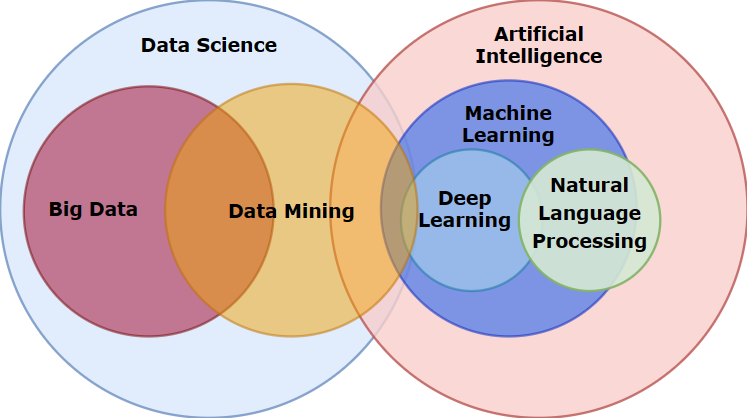
\includegraphics[scale=0.5]{Figuras/diagrama_IA_2.png}
    \caption{Mapa conceptual IA - Ciencia de Datos}
    \label{fig:diagrama_ia}
\end{figure}

\begin{description}
    \item[Inteligencia Artificial] (Artificial Intelligence, AI) disciplina que busca crear algoritmos y sistemas que puedan imitar a la inteligencia humana para realizar tareas complejas de forma autónoma, por ejemplo percepción, toma de decisiones o aprendizaje.
    \item[Aprendizaje Automático] (Machine Learning, ML) conjunto de algoritmos dentro del ámbito de la inteligencia artificial que son capaces de identificar y reconocer patrones en conjuntos de datos para realizar predicciones u otras tareas, descubriendo, por si solos, relaciones entre las variables sin haber sido programados explícitamente para ello, si no a base de tratar con un gran volumen de datos o ejemplos.\\ Machine Learning es un término originado en los años 1950, definido por primera vez por Arthur Lee Samuel, informático teórico estadounidense. Tom Mitchell, informático teórico posterior, llegó a proponer la siguiente definición, más precisa: \textit{Un programa se dice que aprende de la experiencia \emph{E} con respecto a una tarea \emph{T} y una métrica de desempeño \emph{P}, si su rendimiento en \emph{T}, medido por \emph{P}, mejora con la experiencia \emph{E}}.

    \item De estas dos definiciones podemos concluir que el Aprendizaje Automático es una manera de Inteligencia Artificial. De todos modos, podemos tener AI sin ML; por ejemplo, si codificamos reglas, árboles de decisión o técnicas de búsqueda, podemos crear un agente heurístico de inteligencia artificial, sin un enfoque basado en el del ML.
    \item[Aprendizaje Profundo] (Deep Learning, DL) técnica de ML que imita redes neuronales de manera artificial para aprender a partir de datos no estructurados, consiguiendo una mayor capacidad de representación que otras técnicas de ML tradicional.
    \item[Ciencia de Datos] (Data Science) campo interdisciplinario que utiliza métodos estadísticos, de programación y de análisis de datos para extraer conocimiento de conjuntos de datos.
    \item[Grandes conjuntos de datos] (Big Data) término usado para el almacenamiento y procesado de grandes volúmenes de datos.
    \item[Minería de Datos] (Data Mining), subconjunto de la Ciencia de Datos especializado en los procesos de extracción de información útil de grandes conjuntos de datos en bruto estructurados y heterogéneos.
\end{description}

Las técnicas exploradas y desarrolladas en este Trabajo Final de Grado corresponden a un área dentro del \textit{Aprendizaje Automático} relativamente reciente, llamado \textit{Aprendizaje Federado}, por lo que las siguientes secciones se centrarán en profundizar en los fundamentos de ambas, así como en las técnicas de procesado de datos y preparación de los mismos, que son tan fundamentales para un buen desempeño como la idoneidad o eficacia del propio algoritmo.

\subsection{Aprendizaje automático}
El aprendizaje automático nace con la idea de buscar algoritmos que hagan posible que los ordenadores puedan \textit{aprender}{ }--{ }sin ser programados para seguir unas reglas específicas dictadas de antemano{ }--{ }a través de la experiencia; partiendo de un gran volumen de ejemplos.

Estos ejemplos formarán lo que se conoce luego como datos de entrada y, más específicamente, predictores o características (\textit{features or predictors}). Así, los algoritmos de ML se usan para descubrir patrones ocultos, establecer relaciones y grupos o predecir algún atributo.

De lo anterior se puede concluir que el \textit{Machine Learning} se puede usar para la resolución de problemas que no estén determinados con fórmulas precisas y que, por tanto, se podrían reducir a un planteamiento basado en sistemas de reglas; si no para aquellos donde se desconozca la correspondencia entre causas y efectos, bien por la gran cantidad de variables dependientes, bien por la complejidad o aleatoriedad de las mismas.

Las técnicas de ML hacen un uso conjunto de distintas áreas de conocimiento para lograr sus objetivos, como la estadística, probabilidad, cálculo y optimización mediante métodos numéricos. Además, también se inspira en otras disciplinas como la teoría de la información, la psicología o la neurociencia.

Antes de introducir el tipo de aprendizaje automático que nos incumbe, el caso \textbf{supervisado}, que abordaremos más adelante, se va a introducir ahora la terminología necesaria y también una aproximación general al funcionamiento de un método típico de ML.

La figura \ref{fig:procesado_ML} ilustra, de forma simplificada, la terminología y la metodología empleada en el flujo de trabajo de un método genérico de \textit{aprendizaje automático}, donde se recogen unos datos brutos, se procesan, y son alimentados al modelo divididos en conjuntos para su  entreno, validación y optimización. Una vez satisfechos con el rendimiento y eficacia dadas por las métricas de evaluación se considera el modelo listo y se procede a su despliegue.

\begin{figure}[h!]
    \centering
    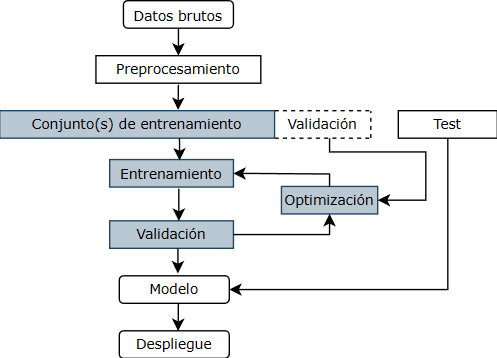
\includegraphics[height=0.4\textwidth, width= 0.8\textwidth]{Figuras/flujo_ml_abel.png}
    \caption{Flujo de procesado en métodos de Machine Learning}
    \label{fig:procesado_ML}
\end{figure}

Existen varios tipos de aprendizaje automático, pero sin duda hay tres grandes categorías, el \textbf{aprendizaje supervisado}, el \textbf{no supervisado} y \textbf{por refuerzo}. La figura \ref{fig:categorias_ml} muestra esta división y las entradas y salidas típicas correspondientes para cada una de ellas.

%figura sl_ul_rl
\begin{figure}[H]
    \centering
    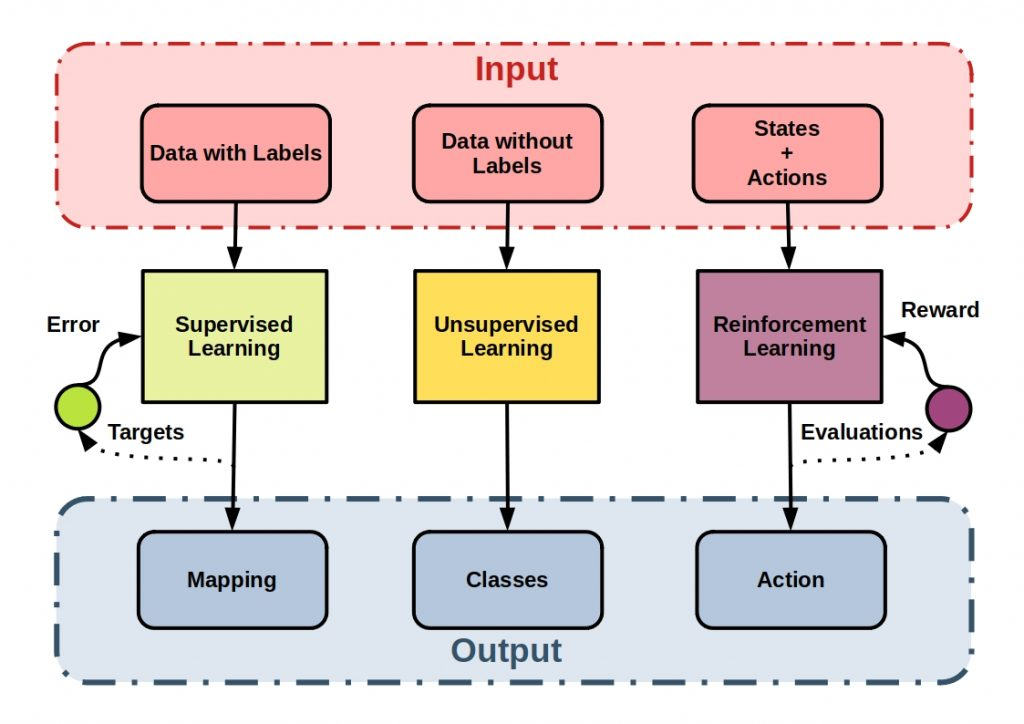
\includegraphics[scale=0.5]{Figuras/unsupervised_supervised_reinforcement.jpeg}
    \caption{Resumen de las tres categorías principales en Aprendizaje automático \cite{starship_ML}}
    \label{fig:categorias_ml}
\end{figure}

\subsubsection{Aprendizaje supervisado}
Como sugiere el nombre, el aprendizaje para estos métodos está supervisado porque se basa en un atributo u objetivo específico del que se tiene constancia, es decir, que se encuentra correctamente etiquetado.

Así, el conjunto de datos consta de un atributo objetivo etiquetado que se encuentra acompañado de otras variables que se usarán para predecirlo, denominadas \textit{predictores} o \textit{características}.

El objetivo puede ser un atributo numérico continuo o un atributo de clases para representar múltiples categorías. Basado en la anterior división, se habla entonces de tareas de aprendizaje supervisado de \textbf{regresión} o \textbf{clasificación}, respectivamente.

Como se muestra en la parte superior de la figura \ref{fig:clasificacion_regresion}, la regresión intenta ajustar los datos a una serie de valores continuos, mientras que la clasificación, en la parte inferior, trata de separar el conjunto de datos en clases.

%lista algoritmos
Existen muchos algoritmos de aprendizaje automático dentro de esta categoría, por mencionar algunos de ellos:
\begin{itemize}[noitemsep, topsep=5pt]
    \item Regresión logística.
    \item Regresión lineal.
    \item Árboles de decisión.
    \item K-vecinos más cercanos.
    \item Bosques aleatorios.
    \item Máquinas de Vectores soporte.
    \item Redes de neuronas artificiales (RNA).
\end{itemize}

%figura ejemplo
\begin{figure}[H]
    \centering
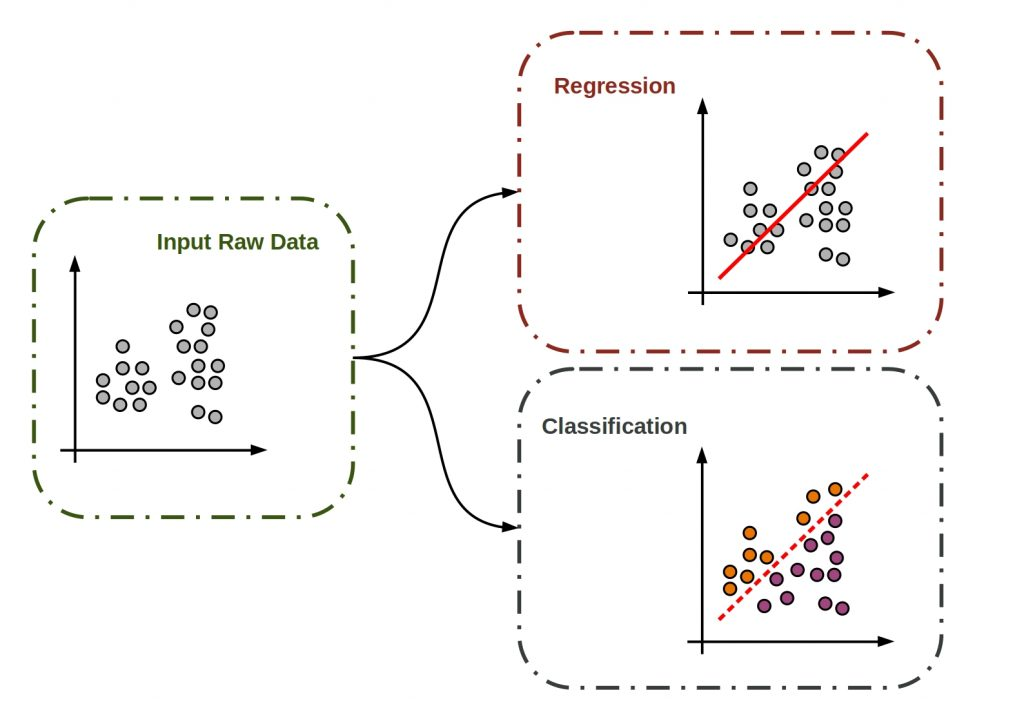
\includegraphics[scale=0.4]{Figuras/clasificacion_regresion.jpeg}
    \caption{Tareas de clasificación y regresión en aprendizaje supervisado \cite{starship_ML}}
    \label{fig:clasificacion_regresion}
\end{figure}

\subsubsection{Aprendizaje no supervisado}
En el caso del aprendizaje no supervisado, no existe un atributo objetivo, es decir, no se cuenta con datos etiquetados. El fin de estos métodos es el de identificar patrones deduciendo la estructura y relaciones que tienen los atributos del conjunto de datos entre sí, separándolos en diferentes grupos o \textit{clusters}. Existen dos grandes tipos de problemas que resuelven estas técnicas, la segmentación (\textit{clustering}) y la reducción dimensional.

En la mitad superior de la figura \ref{fig:clasificacion_ML} se ilustra cómo la segmentación agrupa los datos en diversos conjuntos según características similares que encuentre entre ellos, mientras que, en la mitad inferior, se aprecia cómo la reducción dimensional intenta comprimir, en un número menor de variables, e intentando perder la mínima información posible, el conjunto de datos.

Entre las aplicaciones prácticas típicas de estas técnicas estarían la agrupación de clientes, recomendación de productos y extracción de componentes principales.

%figura ejemplo
\begin{figure}[H]
    \centering
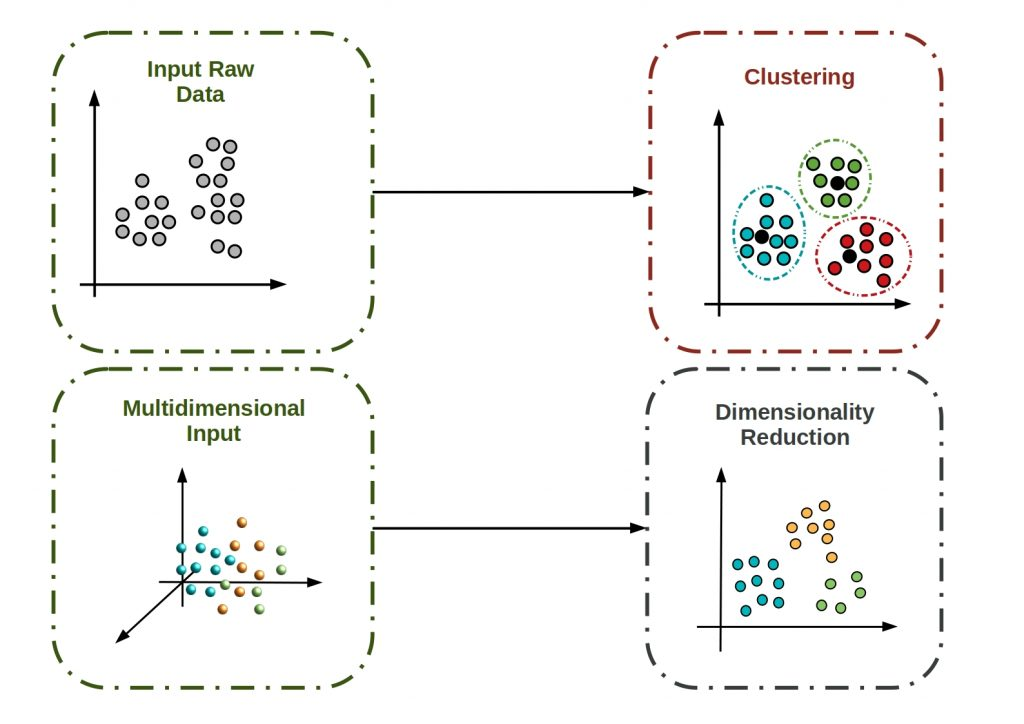
\includegraphics[scale=0.4]{Figuras/clasificacion_ML.jpeg}
    \caption{Tareas de aprendizaje no supervisado: segmentación y reducción dimensional \cite{starship_ML}}
\label{fig:clasificacion_ML}
\end{figure}

%listado algoritmos
Algunos de los algoritmos usados para este fin son:
\begin{itemize}[noitemsep]
    \item K-medias.
    \item Clustering espectral.
    \item Clustering jerárquico.
    \item Análisis de componentes principales (\textit{Principal Component Analysis, PCA}).
    \item Descomposición en valores singulares (\textit{Singular Value Decomposition, SVD}).
\end{itemize}

\subsubsection{Aprendizaje por refuerzo}
En esta categoría de aprendizaje automático existe un agente que interactúa con un entorno y que aprende la toma de decisiones que maximice una recompensa numérica dada por el modelo. Como se observa en la figura \ref{fig:flujo_refuerzo}, el agente \textit{aprende} a través de la prueba y error de manera iterativa, recibiendo información sobre el éxito o fracaso de sus \textit{acciones} mediante \textit{recompensas} o penalizaciones, de forma que existe una retroalimentación entre agente y el entorno.

%piezas clave
Los conceptos clave en el aprendizaje por refuerzo (Reinforcement Learning, RL) son el agente (algoritmo ML), el entorno (espacio de problemas adaptativo), la acción (paso que el agente realiza para navegar por el entorno), el estado (situación del entorno en un momento dado), la recompensa o castigo (recibido por realizar una acción) y la recompensa acumulada (suma de todas ellas). El objetivo es así el de encontrar una estrategia que maximice la recompensa acumulada a largo plazo ya que, en general, existe siempre una mediación entre la exploración del entorno, la selección de acciones y la actualización de la política o función de valor correspondiente.


%figura
\begin{figure}[H]
    \centering
    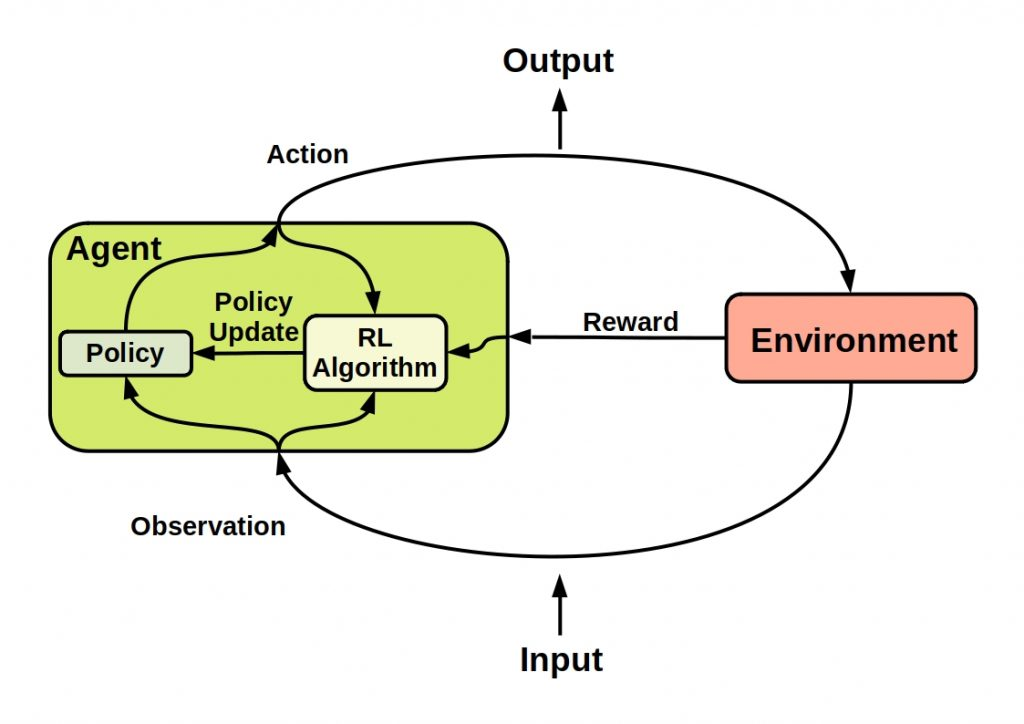
\includegraphics[scale=0.4]{Figuras/reinforcement_ML.jpeg}
    \caption{Flujo de trabajo de los métodos de aprendizaje por refuerzo \cite{starship_ML}}
    \label{fig:flujo_refuerzo}
\end{figure}

%algoritmos
En cuanto a los algoritmos típicos de esta categoría de aprendizaje, tenemos:
\begin{itemize}[noitemsep]
    \item Aprendizaje-Q.
    \item Método de gradiente de políticas.
    \item Métodos Montecarlo.
    \item Aprendizaje por diferencia temporal.
\end{itemize}

%tipos
Todos ellos se pueden agrupar en dos categorías, el RL \textit{basado en modelos}, cuando el entorno está bien definido e invariable, y el RL \textit{sin modelo}, cuando el entorno es grande, complejo, desconocido o cambiante.
%aplicaciones
Este tipo de métodos se usan comúnmente en problemas de toma de decisiones secuenciales y condicionales.

\subsubsection{Desarrollo de modelos}
\label{sec:Desarrollo_de_modelos}
En esta sección abordamos conceptos generales de \textit{Aprendizaje Automático} que se han de tener en cuenta a la hora de desarrollar un modelo, además de los pasos y flujos necesarios para llevarlos a cabo.

En general, el desarrollo de un modelo de \textbf{ML} implica siempre las siguientes fases, tal y como se ilustran en la figura \ref{fig:flowchart_ml}:

\begin{enumerate}[noitemsep]
    \item \textbf{Definir} y entender el problema.
    \item \textbf{Recopilar} datos.
    \item \textbf{Preparar} datos.
    \item \textbf{Seleccionar} el algoritmo apropiado y construir el modelo.
    \item \textbf{Evaluar} y optimizar el modelo.
    \item \textbf{Desplegar} para uso práctico.
\end{enumerate}

\begin{figure}[H]
    \centering
    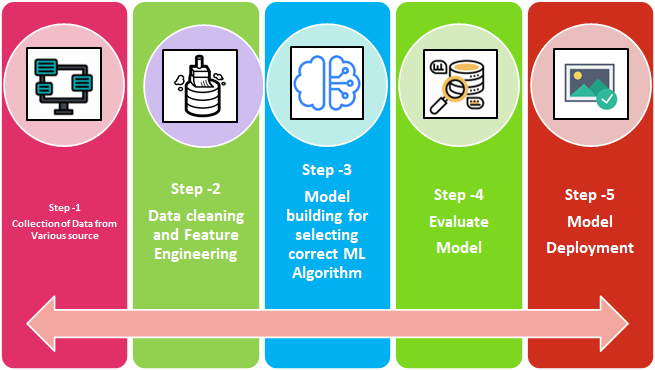
\includegraphics[scale=0.7]{Figuras/flow_chart_ml.png}
    \caption{Flujo de desarrollo típico de un modelo de \textit{ML} \cite{flujo_ML}}
    \label{fig:flowchart_ml}
\end{figure}

\subsubsection*{\centering\textcircled{1} Definición del problema}
Es muy importante empezar entendiendo el problema a resolver y las necesidades y características del mismo; \textit{¿que objetivo buscamos?}. Para lograr una aplicación y uso satisfactorio hay que definir bien los datos disponibles, el tipo de problema y los requisitos de su solución. 

Así, los datos disponibles pueden estar en varias localizaciones, generarse en tiempo real, presentar múltiples formatos y necesitar más o menos preprocesamiento. El tipo de problema puede ser uno de predicción de valores, clasificación, agrupación, reconocimiento de voz, imágenes, etc. Los requisitos de la solución son aquellos requerimientos de negocio que necesite cumplir el modelo final, ya que no sirve de nada construir un modelo que luego no pueda cumplir en cuestión de tiempo de respuesta/disponibilidad/veracidad las necesidades iniciales.

\subsubsection*{\centering\textcircled{2} Recopilación de datos}
La recogida de datos de una o varias fuentes necesita satisfacer los requerimientos del problema y del modelo, que puede llegar a necesitar un gran volumen de datos representativos para ser capaz de descubrir los patrones y las relaciones entre ellos.

El formato de los datos y la estructura precisada para posteriores fases es trabajo para este ciclo del desarrollo, que muchas veces echa mano de técnicas de grandes conjuntos de datos (\textit{Big Data}) para lograrlo.

\subsubsection*{\centering\textcircled{3} Preparación de datos}
%data pre-processing
La preparación de datos o \textbf{preprocesamiento} de datos es uno de los pasos críticos, si no el que más, a la hora de construir un modelo de \textit{Aprendizaje Automático} eficaz, ya que no sólo dispone el conjunto de datos de tal modo que puedan ser alimentados al modelo, si no que también se encarga de su tratamiento para que estos arrojen unos resultados satisfactorios, adaptándose a las necesidades del modelo y a los requisitos de negocio.

El preprocesamiento de datos alberga dos grandes fases, que son la \textbf{transformación de datos} y la \textbf{selección/generación de características}. A grandes rasgos, la primera atañe, para \textit{valores numéricos}, su escalado, tratamiento de datos faltantes y atípicos y su agrupamiento, mientras que para \textit{valores categóricos} concierne su codificación y tratamiento de valores faltantes. La segunda fase trata de seleccionar aquellos atributos y características representativas del problema, filtrar los datos incompletos o generar datos nuevos si fuese necesario.

Esta preparación de datos incumbe toda una serie de pasos que se describen{ }--{ }superficialmente{ }--{ }a continuación:
\begin{enumerate}[itemsep=2pt]
    \item \textbf{Limpieza de datos}: consiste en eliminar datos incompletos, irrelevantes y, en general, la transformación del conjunto a un formato uniforme y coherente.
    \item \textbf{Exploración de datos}: se realiza un primer análisis del conjunto de datos para visualizar patrones, tendencias, correlaciones entre variables e identificar valores atípicos o \textit{outliers} (valores que se salen de una medida del rango intercuartílico adoptada), los cuales se suelen o bien eliminar del conjunto o bien sustituir por datos acotados (técnicas \textit{trimming}/\textit{winsorizing} respectivamente).
    \item \textbf{Selección de características}: efectuado el anterior análisis, se deberían de filtrar ahora las características/atributos más relevantes y significativos, y descartar aquellos cuya correlación es nula o irrelevante, para ayudar a la convergencia en el entrenamiento del modelo y mejorar así su precisión en las predicciones.
    \item \textbf{Tratamiento de valores faltantes} (\textit{missing-values}): en gran parte de escenarios se encuentran observaciones donde faltan alguna de las características muestreadas, por lo que se suele llevar a cabo una de las siguientes acciones: eliminación de la observación o reemplazo por una constante global/media/mediana.
    \item \textbf{Balanceamiento de datos}: repercute, sobre todo, a problemas de clasificación en aprendizaje supervisado, ya que es común encontrarse con datos en los que una de las clases tiene menos muestras que el resto. Estos casos de conjuntos desequilibrados se suele remediar mediante métodos como el \textit{down-sampling} o \textit{over-sampling}. El primero reduce el número de muestras de las clases mayoritarias y el segundo aumenta el número de muestras de la clase minoritaria (duplicando o creando datos nuevos) hasta equilibrarlas.
    \item \textbf{Codificación de datos}: en este paso se realiza la transformación de datos para su entrada al modelo y mejorar así su rendimiento. Incluye etapas de escalado y normalización, usando técnicas como \textit{estandarización Z-score} o \textit{normalización min-max}, además de realizar la codificación de datos categóricos, usando por ejemplo \textit{one-hot encoding}, o, también, el agrupamiento o \textit{binning} de valores numéricos, incluyendo además posibles transformaciones logarítmicas o exponenciales que ayuden al modelo.
    \item \textbf{División de datos}: paso fundamental y necesario en el desarrollo de todo modelo, y por el cual se fragmenta aleatoriamente el conjunto de datos preprocesado en tres conjuntos, \textbf{entrenamiento}, \textbf{validación} y \textbf{test}, en unas determinadas proporciones, normalmente un $60\%-20\%-20\%$ correspondientemente. El modelo aprende con los datos de entrenamiento, optimiza configuraciones y evalúa con los de evaluación y prueba con los de test.
    %figura
    \begin{figure}[H]
        \centering
        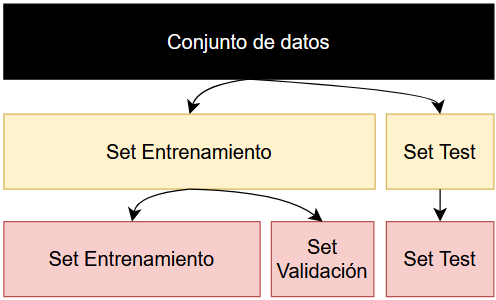
\includegraphics[scale=.9]{Figuras/train_test_split.png}
        \caption{Esquema de la división de datos en \textit{sets} de entrenamiento, validación y test}
        \label{fig:train_test_split}
    \end{figure}
\end{enumerate}

La división en conjuntos de entrenamiento y test independientes sería suficiente para evaluar la precisión del modelo, pero no se asegura así que se haya generalizado bien el problema y no simplemente 'memorizado' las salidas necesarias.

Un método popular y más robusto todavía de división de datos es el llamado de \textbf{validación cruzada}, y una de sus técnicas más populares se conoce por \textit{K-fold cross-validation}, donde el set de entrenamiento se divide en $k$ submuestras de igual tamaño. Durante el entrenamiento, $k-1$ muestras se usan para entrenar el modelo y la restante para validarlo. Esto se repite $k$ veces con cada una de las submuestras restantes, de manera que se garantiza que los datos de entrenamiento y validación se van rotando durante la optimización del modelo. Los resultados de la evaluación se combinan mediante media aritmética para conseguir la estimación oportuna, como se ilustra en la figura \ref{fig:kcrossvalidation}.

%figura
\begin{figure}[H]
    \centering
    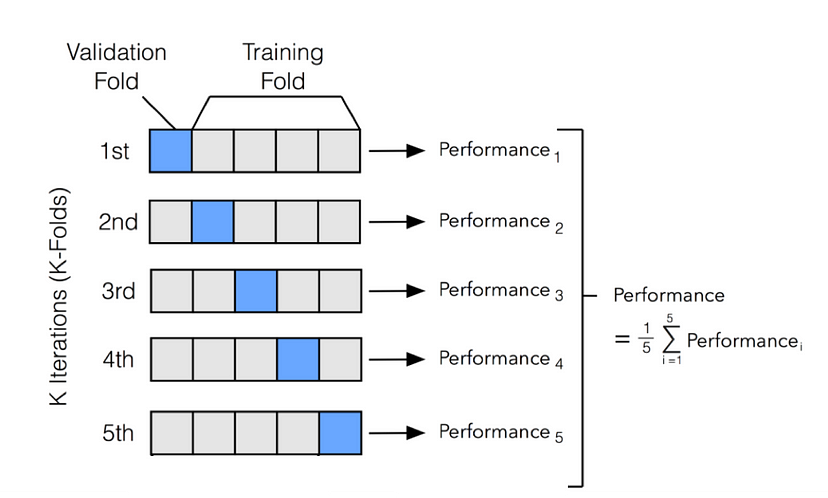
\includegraphics[scale=0.5]{Figuras/k_cross_validation.png}
    \caption{División y uso del método de validación cruzada \textit{K-fold} \cite{kcross}}
    \label{fig:kcrossvalidation}
\end{figure}

Con esta división o \textit{preprocesamiento} del conjunto de datos se pretende que el \textit{dataset} obtenido sea \textbf{representativo}, para obtener un modelo eficaz y sacar predicciones útiles del mismo. Esto significa, entre otras cosas, evitar el \textbf{overfitting} o sobreajuste y el \textbf{underfitting} o infraajuste del modelo, y escapar así del conflicto que existe entre \textit{optimización} y \textit{generalización}. El sobreajuste ocurre cuando se entrena demasiado un modelo del cual se conocen sus salidas deseadas, 'memorizando' pautas que son demasiado específicas de los datos de entrenamiento e irrelevantes para datos nuevos, como se aprecia en la figura \ref{fig:overfitting1}. Infraajuste es cuando ocurre todo lo contrario, y el modelo carece de capacidad de representación para ajustarse a las necesidades del \textit{dataset}.

%fig
\begin{figure}[H]
    \centering
    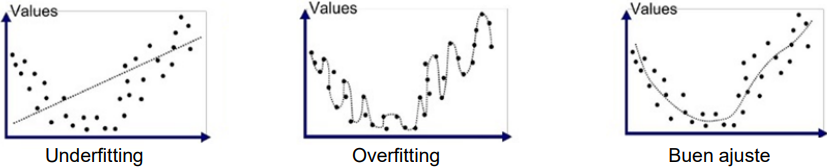
\includegraphics[width=\textwidth]{Figuras/overfitting.png}
    \caption{Gráficas simplificadas representando tres escenarios: \textit{infraajuste}, \textit{sobreajuste} y ajuste deseado \cite{overfitting}}
    \label{fig:overfitting1}
\end{figure}

Un indicador de que se está produciendo sobreajuste es cuando, luego de descender ambos, el error del conjunto de validación empieza a crecer, o estancarse, mientras que el error sobre el conjunto de entrenamiento sigue bajando, como se observa en la figura \ref{fig:overfitting2}.

%fig
\begin{figure}[H]
    \centering
    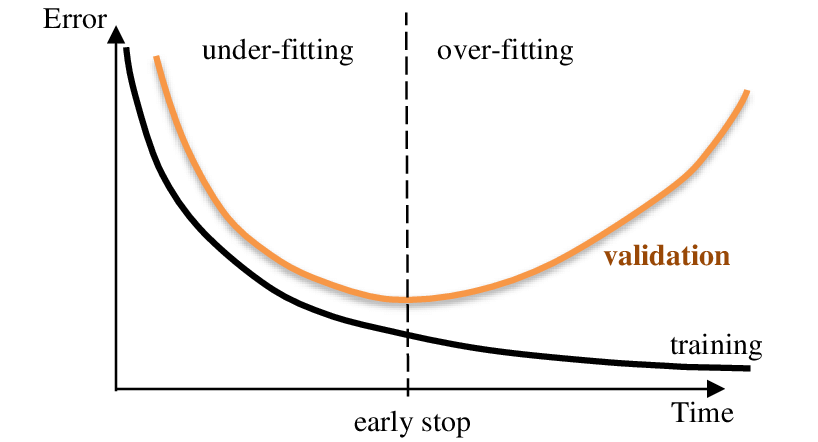
\includegraphics[scale=0.4]{Figuras/overfitting_2.png}
    \caption{Gráfica mostrando el proceso de sobreajuste basado en los errores de validación y entrenamiento \cite{overfitting2}}
    \label{fig:overfitting2}
\end{figure}

Para evitar el sobreajuste existen técnicas sencillas y complejas. La más sencilla de todas es la llamada \textit{early-stopping}, que significa detener el entrenamiento una vez que se observan tendencias distintas en los errores de la figura \ref{fig:overfitting2}. Otra de fácil implementación sería la propia \textit{validación cruzada} que se explicó antes. Por último, la llamada \textbf{regularización} consiste en reducir la complejidad global del modelo, a costa de su varianza. Técnicas de este estilo incluyen la regularización \textit{L1}, \textit{L2}, \textit{Lasso} o \textit{Ridge}.

\subsubsection*{\centering\textcircled{4} Selección y construcción del modelo}
A estas alturas, la selección del algoritmo apropiado y el tipo, estructura y conjunto de datos de trabajo que este necesita ya debería de estar listo, puesto que su tratamiento, división e incluso transformación{ }--{ }muchas veces específica al algoritmo, ya que puede funcionar mejor con según que tipo de entradas{ }--{ }ya se ha abordado en las fases de preparación de datos.

Así, este aspecto de construcción del modelo implica el diseño de su arquitectura y puesta en marcha.

En cuanto a su diseño, se puede optar por arquitecturas centralizadas o distribuidas. Un diseño centralizado implica un modelo donde todo el procesamiento de datos{ }--{ }y su entrenamiento{ }--{ }se realiza en un solo lugar, como una única máquina o servidor. Por la contra, las arquitecturas distribuidas dividen este proceso en varias máquinas o servidores, lo que permite realizar su tratamiento en paralelo y en diferentes lugares geográficos. Este último enfoque se ha de tener en cuenta si existe una necesidad de procesar grandes cantidades de datos en un tiempo razonable, además de si, por la naturaleza del problema, la recogida de datos y su almacenamiento presenta límites físicos o incluso legales que se han de considerar. El diseño también puede llevar consigo el propio dimensionamiento del modelo, sobre todo cuando se trabaja con técnicas de Aprendizaje Profundo (\textit{Deep Learning}, DL), donde la decisión del número de capas ocultas, el número de neuronas por capa y las funciones de activación asignadas a estas es una parte tan fundamental como el propio conjunto de datos y la solución deseada.

Por último, la puesta en marcha de un modelo no garantiza su eficacia ni éxito, y muchas veces es necesario probar con distintos algoritmos y diseños para quedarse con el que presente mejores resultados y desempeño.

\subsubsection*{\centering\textcircled{5} Evaluación y optimización}
La evaluación y optimización del modelo significa la introducción de las métricas de desempeño, la función de coste o pérdida y la afinación de hiperparámetros pero, ¿que son? y, ¿para que sirven?:

\paragraph*{Métricas} Las métricas de desempeño son una serie de indicadores del rendimiento del modelo, de su eficacia, de como de 'bueno' es y, en general, de qué cantidad de error ha cometido cuando se evalúa contra el conjunto de datos de test o de validación.

Existen muchas métricas de desempeño diferentes, pero generalmente se suelen dividir según el tipo de método de aprendizaje automático que se utilice. Así, por ejemplo, hay métricas propias de técnicas de aprendizaje supervisado, no-supervisado y por refuerzo. A continuación desglosamos las más utilizadas para el caso supervisado, que es el que nos incumbe en este trabajo.

\vspace{1em}

\textbf{Aprendizaje supervisado}

\vspace{.5em}

Dado un conjunto de datos $D$ de $n$ muestras, $y\,\in\mathbb{R}^n$ el vector cuyas componentes $y_j$ representan las observaciones o salidas reales de dicho conjunto, $\bar{y}$ el promedio de los valores anteriores e $\hat{y}\,\in\mathbb{R}^n$ el vector cuyas componentes $\hat{y}_j$ son las predicciones resultante del modelo. Para evaluar modelos de \textbf{regresión} se suelen emplear las siguientes métricas:

\begin{itemize}[noitemsep]
    \item MAE, \textit{Mean Absolute Error}, es el error absoluto medio entre los valores reales y la predicción.
    \[MAE = \frac{1}{n} \sum_{j=1}^n |y_j - \hat{y}_j|\]
    \item RMSE, \textit{Root Mean Squared Error}, es el error cuadrático medio entre observaciones y predicciones.
    \[RMSE = \sqrt{\frac{1}{n} \sum_{j=1}^n (y_j - \hat{y}_j)^2}\]
    \item $R^2$, conocido como coeficiente de determinación, aplicado a la relación entre valores reales y predicciones y la varianza total respecto al promedio.
    \[R^2 = 1 - \frac{\sum_{j=1}^n (y_j - \hat{y}_j)^2}{\sum_{j=1}^n (y_j - \bar{y})^2}\]
\end{itemize}

\vspace{0.5em}

Para evaluar modelos de \textbf{clasificación} se determinan una serie de métricas basándose, primero, en los datos aportados por la denominada \textit{matriz de confusión}, que se construye enfrentando en una tabla, de tantas filas y columnas como número de clases exista en el conjunto de datos, la contabilidad de los casos reales y los predichos, produciéndose cuatro tipos de categorías distintas:

\begin{itemize}[noitemsep]
    \item Verdadero Positivo (True Positive, TP): El valor real es positivo y la prueba predijo que también lo era.
    \item Verdadero Negativo (True Negative, NP): El valor real es negativo y la prueba predijo lo mismo.
    \item Falso Positivo (False Positive, FP): El valor real es negativo pero la prueba predijo que era positivo, conocido como \textit{error tipo-I}. 
    \item Falso Negativo (False Negative, FN): El valor real es positivo y la prueba predijo que era negativo, conocido como \textit{error tipo-II}.
\end{itemize}

En la figura \ref{fig:matriz_confusion} se puede observar un ejemplo de esta matriz.

\begin{figure}[H]
    \centering
    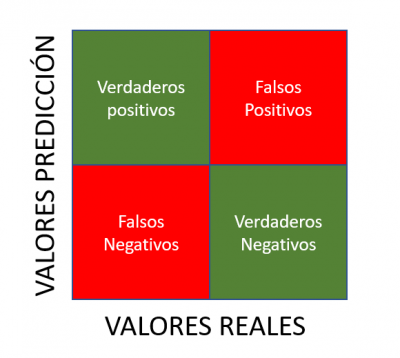
\includegraphics[scale=0.6]{Figuras/matriz_confusion.png}
    \caption{Esquema de la matriz de confusión \cite{matriz_conf}}
    \label{fig:matriz_confusion}
\end{figure}

Una vez contabilizada la matriz anterior, existen una serie de parámetros para validar el desempeño del modelo. Los más reconocidos son:

\begin{itemize}[noitemsep]
    \item \textit{Accuracy}: Medida de exactitud. Para el total de datos, ¿cuantos son ciertos?
    \[Accuracy = \frac{(TP+TN)}{Total}\]
    \item \textit{Precision}: Medida de precisión. Para los casos que el modelo ha clasificado como positivos, ¿cuantos son ciertos?
    \[Precision = \frac{TP}{TP+FP}\]
    \item \textit{Recall}: Medida de sensibilidad. Para los casos reales positivos, ¿cuantos predice?
    \[TPR = \frac{TP}{TP+FN}\]
    \item \textit{Specificity}: Medida de particularidad. Para los casos reales negativos, ¿cuantos predice?
    \[Specificity = \frac{TN}{TN+FP}\]
    \item \textit{F1 Score}: Puntuación F1. Combina precisión y sensibilidad en uno para tener en cuenta positivos dados como ciertos y reales omitidos.
    \[F1_{score} = \frac{2 \cdot Precision \cdot Recall}{Precision+Recall}\]
    \item \textit{False Positive Rate}: Ratio de falsos positivos. El complementario de la particularidad.
    \[FPR = 1-Specificity = 1 - \frac{TN}{TN+FP} = \frac{(TN+FP)-TN}{TN+FP}=\frac{FP}{TN+FP}\]
\end{itemize}

\paragraph*{Función de coste}
También llamada función de pérdida, se usa en algoritmos de aprendizaje supervisado para cuantificar como de buenas son las predicciones de un modelo, de manera que esta función calcula un valor que refleja el error o discrepancia entre ambas.

Durante el entrenamiento, el objetivo es siempre \textbf{minimizar} dicha función, ajustando los pesos o parámetros del modelo para que sus predicciones sean lo más similares posibles a los valores reales. La elección de la función de coste, y su optimización, depende del tipo de problema y algoritmo empleado.

Aunque existen algoritmos de métodos lineales cuya función de coste permiten una resolución no iterativa y cerrada del mismo, como en el método base de este trabajo FedHEONN, en la mayoría de casos se suele recurrir a métodos numéricos para optimizar dicha función de manera iterativa hasta una esperada convergencia a un mínimo, o al criterio de parada especificado.

Las funciones de pérdida comunes incluyen el \textit{MSE} visto antes, la entropía cruzada (en redes neuronales) o la precisión, y los métodos numéricos de optimización usados varían desde descenso de gradiente estocástico (\textit{SGD Stochastic Gradient Descent}), ADAM (\textit{Adaptative Moment Estimation}), entre muchos otros.

\vspace{.5em}

A continuación se ilustra uno de estos procesos de minimización en la figura \ref{fig:gradient}.

%figura loss function y gradiente descent
\begin{figure}[H]
    \centering
    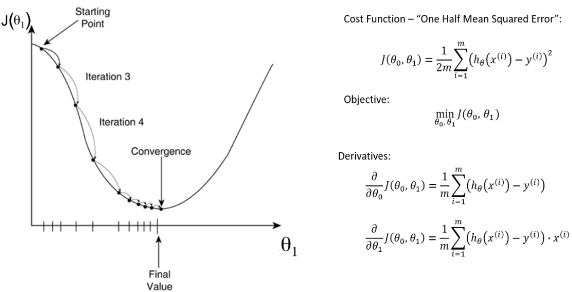
\includegraphics[scale=1.2]{Figuras/gradient.png}
    \caption{Ejemplo de resolución iterativa, por gradiente descendente, de una función de pérdida usada en regresión basada en el MSE \cite{gradient_descent}}
    \label{fig:gradient}
\end{figure}

\paragraph*{Hiperparámetros}
Se conocen como hiperparámetros todos aquellos factores que se establecen antes del proceso de entrenamiento del modelo y que no se \textit{aprenden} directamente de los datos. Estos parámetros controlan la configuración, comportamiento y diseño del algoritmo de aprendizaje, y su ajuste es crucial a la hora de obtener un buen rendimiento del modelo.

A diferencia de los pesos o parámetros del modelo, que se aprenden durante su entrenamiento y optimización de la función de pérdida, los hiperparámetros son seleccionados por el usuario, como por ejemplo la tasa de aprendizaje, el número de capas ocultas en una red neuronal artificial (RNA), el tamaño del lote de trabajo, el número máximo de iteraciones, la profundidad de un árbol de decisión, etc.

Existen técnicas para buscar qué hiperparámetros ofrecen un mejor rendimiento del modelo; algunas son brutas y sistémicas como la búsqueda en cuadrícula (\textit{grid search}) o aleatoria (\textit{random search}) y otras algo más avanzadas como la basada el algoritmos genéticos. En la figura \ref{fig:hyperparam} podemos ver un ejemplo de este concepto.

\begin{figure}[h]
    \centering
    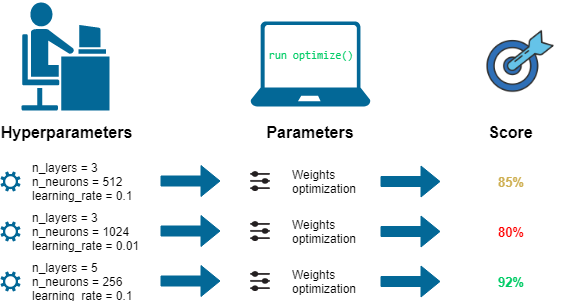
\includegraphics[scale=0.7]{Figuras/hyperparam.png}
    \caption{Ajuste de hiperparámetros para un modelo de aprendizaje supervisado \cite{hyperparam}}
    \label{fig:hyperparam}
\end{figure}

\subsubsection*{\centering\textcircled{6} Despliegue}
El despliegue y uso práctico de un modelo de ML implica la integración del modelo final en un entorno de producción, donde podrá generar los resultados esperados y ser utilizado para la toma de decisiones.

Los únicos factores que se tienen que tener en cuenta aquí son la escalabilidad del modelo, su rendimiento, su capacidad de actualización y mantenimiento, la privacidad y seguridad de los datos y las posibles regulaciones e impacto derivados de su uso.
\newpage

\subsection{Aprendizaje federado}
% Tablas de Kairouz e imagenes de Yang
% subsubsecciones:
% Introduccion -> Motivación, definición (Kairouz y Yang), características, categorias (cross-silo, cross-device, centrado en modelo y centrado en datos), proceso desarrollo (kairouz), privacidad (vulnerabilidades, actores y amenazas, técnicas SMC y DP).
% Tipos -> HFL, VFL, FTL, FRL.
% Aplicaciones y casos de uso, software y datasets.
Con el auge de los dispositivos móviles y otros dispositivos embebidos{ }--{ }de uso doméstico o no{ }--{ }englobados en el llamado \textit{Internet of Things} (IoT) se produce, cada vez más, una abundancia de datos que, siendo adecuados y aprovechables para el entrenamiento de modelos de aprendizaje automático, se desaprovechan por restricciones físicas o éticas, debido a su naturaleza privada o sensible, además de encontrarse distribuidos entre millares de dispositivos desconocidos.

Con esta motivación e ideas de fondo fue como surgió el término de \textit{Federated Learning} o Aprendizaje Federado, acuñado por primera vez en el articulo de McMahan et al. \cite{paper_McMahan} titulado \textit{'Communication-Efficient Learning of Deep Networks from Decentralized Data'}, en donde se da una primera definición y enfoque a la particular casuística y características que atañen a estos modelos.

En dicho artículo se centran específicamente en el caso de los dispositivos móviles, intentando usar los datos contenidos en estos para usarlos en modelos de ML que mejoren la usabilidad de los mismos; como se materializaría{ }--{ }a posteriori{ }--{ }con su implantación en el teclado móvil \textit{Gboard} del SO \textit{Android} para mejorar la predicción de palabras y \textit{emojis} del usuario.

Presentan así una solución al uso de estos datos sensibles y distribuidos{ }--{ }que imposibilitan el enfoque tradicional, es decir, aunarlos en un centro de datos y realizar con ellos el desarrollo del modelo{ }--{ }defendiendo una nueva técnica de aprendizaje que permite a los usuarios aprovechar colectivamente los beneficios de los modelos sin necesidad de almacenar los datos de forma centralizada ni llegar a compartirlos, creando una red federada de dispositivos que resuelva la función objetivo bajo la coordinación de un servidor central.

Cada uno de los dispositivos{ }--{ }o clientes{ }--{ }mantiene su conjunto de datos intacto de forma local y sólo comparte con el servidor unas actualizaciones iterativas de los pesos de sus respectivos modelos locales, que ni siquiera son necesarios guardar en el servidor central una vez aplicados, en completa sintonía con los principios de \textit{focused collection} y \textit{data-minimization} propuestos en el informe de ciberseguridad de la Casa Blanca \cite{paper_WH} de 2013 \textit{'Consumer data privacy in a networked world'}.

\begin{figure}[H]
    \centering
    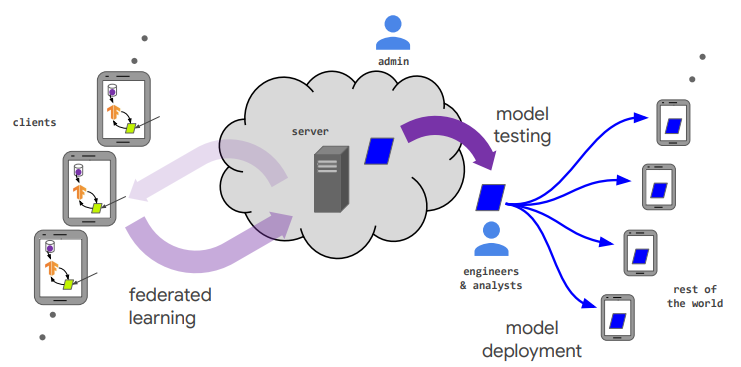
\includegraphics[scale=0.9]{Figuras/fl_kairouz_1.png}
    \caption{Ejemplo de aplicación, ciclo de vida y actores durante el entrenamiento de un sistema de Aprendizaje Federado \cite{libro_kairouz}}
    \label{fig:fl_kairouz_1}
\end{figure}

En resumen, podemos decir que las técnicas de Aprendizaje Federado surgen como solución a los problemas de aislamiento y fragmentación de datos sensibles que, a mayores, requieren, por motivos éticos y legales, adecuarse a restricciones de privacidad y seguridad.

\subsubsection{Definición, características y proceso de desarrollo}

Debido a que, en la primera introducción del término \textit{Federated Learning}, se hizo un enfoque especial a su uso en dispositivos móviles, presentamos una definición más general de este concepto extraída del libro de Kairouz et al. \cite{libro_kairouz} de años posteriores, que lo explica como:

\begin{quote}
    El Aprendizaje Federado es un entorno del aprendizaje automático en el que múltiples entidades (clientes) colaboran en la resolución de un problema de aprendizaje automático, bajo la coordinación de un servidor central o proveedor de servicios. Los datos brutos de cada cliente se almacenan localmente y no se intercambian ni transfieren; si no que, para lograr el objetivo del aprendizaje, se utilizan actualizaciones iterativas destinadas a su agregación inmediata.
\end{quote}

Caben dos apuntes en la definición anterior; la primera, es que estas 'actualizaciones iterativas' tienen el alcance justo y limitado para contener la mínima información necesaria para la tarea de aprendizaje en cuestión{ }--{ }realizando su agregación lo antes posible evitando su almacenaje y posible reconstrucción{ }--{ }y, la segunda, es que no se tiene en cuenta las técnicas de aprendizaje federado totalmente descentralizadas (P2P), que carecen de servidor central y difieren de la arquitectura clásica cliente-servidor de la definición, como ilustra la figura \ref{fig:arq_fl_yang}.

\begin{figure}[H]
    \centering
    \begin{subfigure}{.47\linewidth}
        \centering
        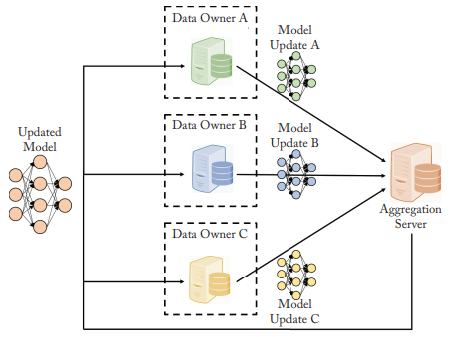
\includegraphics[width=\linewidth]{Figuras/yang_fl_1.png}
        \caption{Modelo \textit{cliente-servidor}}
    \end{subfigure}
    \hfill
        \begin{subfigure}{.47\linewidth}
        \centering
        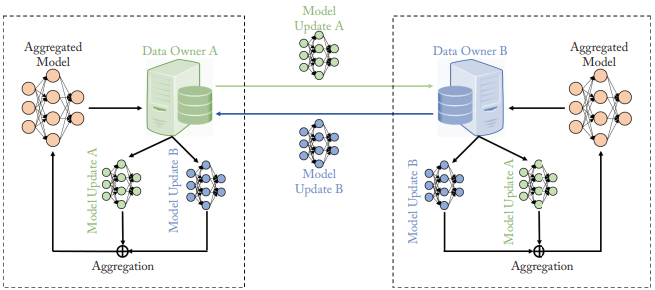
\includegraphics[width=\linewidth]{Figuras/yang_fl_2.png}
        \caption{Modelo \textit{peer-to-peer}}
    \end{subfigure}
    \caption{Arquitecturas en sistemas de Aprendizaje Federado \cite{libro_Yang}}
    \label{fig:arq_fl_yang}
\end{figure}

De uno u otro modo se mantienen los datos de entrenamiento descentralizados, mitigando muchos de los riesgos y costes asociados a la privacidad y derivados del aprendizaje automático tradicional y centralizado que, además, como veremos en futuros capítulos, es menos eficiente energéticamente.

\vspace{1em}

Entre las \textbf{características de los problemas de optimización} a los que se enfrentan las técnicas de aprendizaje federado se encuentran, normalmente, las siguientes:

\begin{itemize}[noitemsep]
    \item \textbf{Distribución estadísticas desiguales y no uniformes}: en estos entornos, no se pueden asumir los supuestos de las técnicas tradicionales de ML distribuido, como son el de conjuntos de datos \textit{IID} (Independent and Identically Distributed), es decir, muestras independientes entre sí y con idénticas distribuciones de probabilidad. Y es que hay que suponer que, aunque cada cliente aporte datos locales correspondientes al mismo objetivo, debido al uso y circunstancias de cada uno, su distribución ha de ser distinta.
    \item \textbf{Desequilibrado de datos}: Por la misma razón que el punto anterior, no se puede suponer que las muestras han de tener tamaños iguales o que contengan el mismo número de datos sobre clases o \textit{clusters} que el resto.
    \item \textbf{Escalabilidad masiva}: debido a que los datos pueden estar distribuidos sobre un gran número dispositivos, es requisito fundamental que estos sean capaces de manejar distribuciones masivas de clientes.
    \item \textbf{Diferencias computacionales}: Debido a la diversidad de dispositivos que pueden conformar estas redes federadas, se ha de tener en cuenta distintas capacidades computacionales, que pueden afectar, dependiendo del hardware disponible, en el número de iteraciones o rondas en las que participe el cliente o el tiempo esperado de respuesta de cada uno de ellos.
    \item \textbf{Comunicaciones costosas}: A diferencia de lo que sucede en escenarios clásicos de computación distribuida, donde existe un gran ancho de banda bajo redes locales, en las redes federadas resulta ser lo contrario, con clientes que no siempre pueden estar disponibles y que usan conexiones lentas y poco fiables, por lo que el modelo tiene que poder gestionar desconexiones e incorporaciones súbitas.
\end{itemize}

Una vez conocidos los principales retos a los que se enfrenta el \textit{problema de la optimización federada}, podemos introducir las fases típicas del \textbf{proceso de entrenamiento} de un modelo de aprendizaje federado:

\begin{enumerate}[noitemsep]
    \item \textbf{Selección de clientes}: El coordinador central o servidor escoge un subconjunto de clientes que cumplan los requisitos apropiados.
    \item \textbf{Difusión}: Los clientes seleccionados obtienen el estado del modelo global actual y su programa de entrenamiento.
    \item \textbf{Cálculos locales}: Cada dispositivo realiza la computación del programa de entrenamiento sobre su conjunto de datos, por ejemplo SGD en un lote local de datos (para un caso de \textit{FedAvg}).
    \item \textbf{Agregación}: El servidor recibe un cúmulo de actualizaciones locales de cada uno de los dispositivos. Los rezagados pueden ser abandonados y no tenidos en cuenta pasado un tiempo máximo. Sobre los disponibles se realiza un promedio ponderado de los pesos obtenidos, según el número de muestras de cada cliente (para un caso de \textit{FedAvg}).
    \item \textbf{Actualización del modelo global}: Por último, el servidor realiza la actualización del modelo global basándose en la agregación anterior.
\end{enumerate}

Cabe decir que, en el flujo anterior, el servidor/coordinador orquesta todo el proceso de entrenamiento (arquitectura cliente-servidor) y el proceso se repite (en caso de ser un modelo iterativo) durante sucesivas rondas hasta que este es detenido debido a su convergencia, número máximo de rondas o agotado el tiempo máximo de entrenamiento.

\subsubsection{Categorías y tipos de aprendizaje federado}
%centrando en modelo y datos
%cross-silo cross-device
%hfl, vfl etc
Existen distintos tipos de categorizaciones presentes en las técnicas de aprendizaje federado, dependiendo del ámbito al que refieran, y que explicaremos brevemente en esta sección.

\vspace{0.5em}

En primer lugar, en referencia al tipo y número de clientes que conforman la red federada, se puede hablar de:

\begin{itemize}[noitemsep]
    \item \textbf{Cross-silo}: reservado para las aplicaciones de FL que involucren a un número reducido de clientes fiables, como por ejemplo, la colaboración entre múltiples organizaciones o entidades en aras de desarrollar un modelo de ML conjunto.
    \item \textbf{Cross-device}: el apropiado para el resto de casos, donde el énfasis está en redes masivas de dispositivos móviles o embebidos (\textit{edge devices}).
\end{itemize}

Por último, basado en la estructura de cada conjunto de datos que participe en la red federada, se habla de:

\begin{itemize}[noitemsep, topsep=5pt]
    \item \textbf{Horizontal Federated Learning, HFL}: el \textit{Aprendizaje Federado Horizontal} representa el caso en el que los conjuntos de datos de cada uno de los clientes comparten una estructura de atributos semejante, como se observa en la figura \ref{fig:hfl}. De este modo, los participantes tienen \textit{datasets} similares en términos de características pero que no pueden ser fusionados debido a restricciones de privacidad o seguridad. Al colaborar y combinar sus modelos locales se logra un modelo global más robusto y generalizado sin revelar los datos sensibles subyacentes.
    \begin{figure}[H]
    \centering
    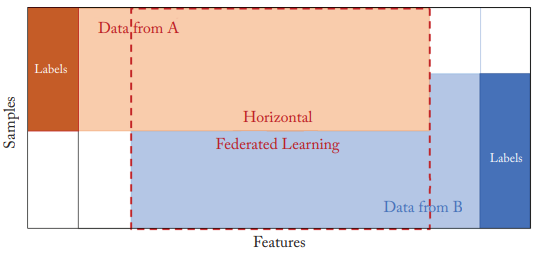
\includegraphics[scale=0.9]{Figuras/hfl_1.png}
    \caption{Estructura de datos compartidas en HFL \cite{libro_Yang}}
    \label{fig:hfl}
    \end{figure}

    \item \textbf{Vertical Federated Learning, VFL}: el \textit{Aprendizaje Federado Vertical} se centra en la colaboración entre múltiples participantes o clientes que poseen características diferentes pero complementarias en sus respectivos conjuntos de datos. Como mínimo, deben tener en común algún tipo de identificador que permita alinear los datos de los distintos conjuntos implicados mediante un proceso criptográfico conocido como \textit{encripted-entity-alignment}. Este escenario es ideal para la colaboración entre múltiples entidades que comparten un grupo de clientes pero donde cada una de ellas tiene información diferente sobre cada uno de ellos. Así, podrían cooperar en el desarrollo de un modelo conjunto que beneficie a ambos sin revelar datos confidenciales de sus clientes el uno al otro.
    \begin{figure}[H]
    \centering
    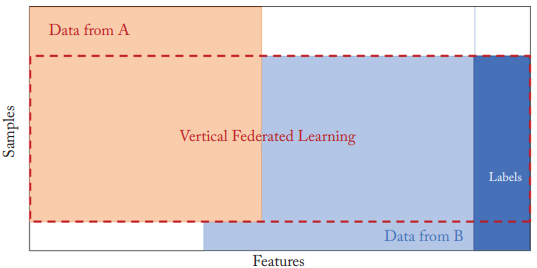
\includegraphics[scale=0.9]{Figuras/vfl_1.png}
    \caption{Estructura de datos complementarios en VFL \cite{libro_Yang}}
    \label{fig:fl_vfl}
\end{figure}
\end{itemize}


\subsubsection{Optimización}
%FedAvg
En esta sección explicaremos, en detalle, uno de los algoritmos de optimización más utilizados en las técnicas de aprendizaje federado y que, a su vez, fue el propuesto inicialmente en el artículo de McMahan et al \cite{paper_McMahan} mencionado al principio del capítulo. Se trata del denominado \textit{FedAvg}, o promedio federado.

Este algoritmo de optimización establece un sistema de actualizaciones síncronas que avanzan en consecutivas rondas de comunicación cliente-servidor. Asume un número fijo de \textit{K} clientes, cada uno con un conjunto de datos local invariable. Al principio de cada ronda, una fracción aleatoria \textit{C} de participantes es seleccionada, y el servidor envia el actual estado global del modelo a cada uno de los clientes (p.ej. pesos de la RNA). Cada cliente realiza entonces el entrenamiento de este aplicado sobre su propio conjunto de datos y envía los resultados de vuelta al coordinador. El servidor agrega estos cambios y el proceso se repite.

\vspace{1em}

Este algoritmo es aplicable a cualquier función objetivo de suma-finita de la siguiente forma, siendo $\bsym{w}$ el vector de parámetros o pesos del modelo y $n$ el número de datos total:

\begin{equation}
\label{eq:1}
\min_{\bsym{w}\,\in\,\mathbb{R}^{d}} f(\bsym{w}) \quad \text{donde} \quad f(\bsym{w}) = \frac{1}{n} \sum_{i=1}^{n}f_i(\bsym{w}) 
\end{equation}

Para los problemas de aprendizaje automático, normalmente $f_i(\bsym{w}) = \ell(x_i, y_i; \bsym{w})$, que es la pérdida en la predicción realizada por $(x_i, y_i)$ con los parámetros del modelo $\bsym{w}_i$. Asumiendo datos particionados entre \textit{K} clientes, con $\mathcal{P}_k$ la serie de índices de las muestras del cliente \textit{k} y $n_k = |\mathcal{P}_k|$, podemos reescribir la ecuación \eqref{eq:1} como:

\begin{equation}
\label{eq:2}
f(\bsym{w}) = \sum_{k=1}^{K}\frac{n_k}{n}F_k(\bsym{w}) \quad \text{donde} \quad F_k(\bsym{w}) = \frac{1}{n_k} \sum_{i\,\in\,\mathcal{P}_k} f_i(\bsym{w})
\end{equation}

Si la partición $\mathcal{P}_k$ se forma distribuyendo uniformemente los datos de entrenamiento entre los clientes de manera aleatoria entonces tendríamos que $\mathds{E}_{\mathcal{P}_k} [F_k(\bsym{w})] = f(\bsym{w})$.

\vspace{1em}

Este supuesto uniformemente distribuido es lo que se conoce como condición \textbf{IID}, y se asume típicamente en algoritmos de optimización distribuidos, aunque, como ya vimos, este algoritmo FedAvg no contempla este caso; es decir, $F_k$ podría ser una mala aproximación aleatoria de $f$, por lo que se trabaja bajo condiciones \textbf{no IID}.

Bajo este tipo de funciones de coste se ha aplicado satisfactoriamente, en aprendizaje automático distribuido, distintas variantes del llamado \textit{Gradiente Descendente Estocástico} o SGD para su optimización, del que \textbf{FedAvg no es si no otra generalización de este}.

\vspace{1em}

El \textbf{SGD} se podría aplicar directamente al problema de optimización federada, donde solo se realice, por ronda, un único calculo de gradiente por lote para aquellos clientes seleccionados; sin embargo, este enfoque es eficiente computacionalmente pero muy costoso en comunicaciones, debido al gran número de rondas necesarias para producir buenos resultados. Por lo tanto, se apostará por realizar múltiples iteraciones (\textit{epochs}) locales con el objetivo de avanzar el aprendizaje y reducir el número total de rondas globales, disminuyendo las rondas de comunicación necesarias para la convergencia, que es el verdadero cuello de botella de estos escenarios. Así, tomando como base el SGD, el algoritmo \textbf{FedAvg} lo generaliza añadiendo tres parámetros: 

\begin{itemize}[noitemsep]
    \item \textit{C}: \textbf{fracción de clientes seleccionados cada ronda}.
    \item \textit{E}: \textbf{número de iteraciones de entrenamiento realizadas en cada cliente sobre su conjunto de datos local}.
    \item \textit{B}: \textbf{tamaño de los lotes de datos locales usados para el entrenamiento}.
\end{itemize}

Cabe mencionar que si $C = 1 \quad E = 1 \quad B = \infty$ entonces FedAvg se convierte sin más en la aplicación de SGD en una red federada, denominada \textbf{FedSVD}.

\vspace{1em}

Cuando se añaden más iteraciones locales de estos cálculos de gradiente por cada cliente ($E \uparrow$) se generaliza, finalmente, a \textbf{FedAvg}, cuyo algoritmo queda esquematizado en el pseudocódigo \ref{alg:fedavg}.

\begin{algorithm}[H]
\caption{\textit{FederatedAveraging}. Los $K$ clientes se indexan por $k$, $B$ es el tamaño de lote local, $E$ el número de iteraciones (\textit{epochs}) locales y $\eta$ la tasa de aprendizaje.}
\label{alg:fedavg}
\begin{algorithmic}[1]
\STATE \textbf{Coordinador o servidor central:}
\STATE inicializa $\bsym{w}_0$
\FOR{cada ronda $t = 1, 2, \dots$}
\STATE $m \leftarrow \max (C \cdot K, 1)$
\STATE $S_t \leftarrow \text{(selección aleatoria de } m \text{ clientes)}$
\FOR{cada cliente $k \in S_t$ en paralelo}
\STATE $\bsym{w}_{t+1}^k \leftarrow \text{ActualizarCliente(}k, \bsym{w}_t \text{)}$
\ENDFOR
\STATE $m_t \leftarrow \sum_{k\,\in\,S_t} n_k$
\STATE $\bsym{w}_{t+1} \leftarrow \sum_{k\,\in\,S_t} \frac{n_k}{m_t}\;\bsym{w}_{t+1}^k$
\ENDFOR
\STATE
\STATE \textbf{ActualizarCliente(}\textit{k}\textbf{, }\textit{w}\textbf{):}
\STATE $\mathcal{B} \leftarrow \text{(Particionar } \mathcal{P}_k \text{ en lotes de tamaño \emph{B})}$
\FOR{cada \textit{epoch} local $i = 1, \dots, E$}
\FOR{cada lote $b \in \mathcal{B}$}
\STATE $\bsym{w} \leftarrow \bsym{w} - \eta \nabla \ell (\bsym{w}; b)$
\ENDFOR
\ENDFOR
\RETURN $\bsym{w} \text{ al servidor}$
\end{algorithmic}
\end{algorithm}

\subsubsection{Amenazas y privacidad de datos}
%Externas-Internas Secure aggregation HE - TEE
Aunque el atractivo propio de las técnicas de FL es que tienen, \textbf{por diseño, una naturaleza privada}, haciendo que los clientes participantes no revelen sus datos sensibles, si no solo actualizaciones de los modelos locales que entrenan{ }--{ }cumpliendo así la filosofía del \textit{data minimization}{ }--{}, esto no quita que sigan siendo vulnerables a cierto tipo de ataques.

\vspace{0.5em}

Podemos distinguir dos escenarios de posibles amenazas:

\begin{itemize}[noitemsep]
    \item \textbf{Global}: encargado de proteger el funcionamiento del sistema federado frente a dispositivos externos maliciosos u \textit{honestos pero curiosos}.
    \item \textbf{Local}: encargado de evitar fugas de información sensible del cliente hacia el servidor durante las comunicaciones que realizan entre sí.
\end{itemize}

Aunque la privacidad no se puede tratar como una cualidad binaria o perfectamente cuantificable, si se puede presentar una serie de objetivos de privacidad para justificar el uso de distintas herramientas y tecnologías en ciertas partes del flujo de trabajo.

Existen tres aspectos de la privacidad de estos sistemas que tienen que ser comprendidos y analizados para saber que tipo de remedio se puede usar para reforzarlos. Podemos imaginar y simplificar el proceso de las técnicas de aprendizaje federado como el de la evaluación de una función $\bsym{f}$ en un conjunto de datos distribuidos en varios clientes. Dada esta analogía, habría que tener en cuenta:

\begin{enumerate}[itemsep=2pt]
    \item Como se calcula $f$ y cual es el flujo de información de los resultados intermedios, ya que estos son susceptibles a un cliente, servidor o administrador malicioso. Además de la privacidad por diseño del propio FL (\textit{data minimization}), aquí se introducen técnicas de computación segura multi-parte (Secure Multiparty Computation, \textbf{SMPC}).
    \item Que es lo que se calcula, es decir, cuanta información sobre un participante se revela a terceros o a los usuarios finales por el resultado del despliegue de $f$. Para contrarrestarlo se aplican métodos de privacidad diferencial (Differential Privacy, \textbf{DP}).
    \item Por último resta la verificabilidad, entendida como la capacidad de un cliente o servidor de probar a otros participantes del sistema que han ejecutado el entrenamiento o programa al que se han comprometido fielmente, sin revelar los datos potencialmente sensibles sobre los que actuaron. Para esto, se hace uso de técnicas conocidas como pruebas de conocimiento cero (Zero-Knowledge-Proofs, \textbf{ZKP}).
\end{enumerate}

A continuación explicamos brevemente algunas de estas técnicas y cuál es la escogida en el algoritmo de partida de este trabajo.

\paragraph*{Secure Multi-Party Computation}\mbox{}\\
%HE
También conocidos como protocolos seguros o computación segura distribuida, se trata de un campo de la criptografía encargado de hacer que una red de participantes calculen una función acordada, con sus datos locales como entradas, de tal manera que solo revelen la salida de estas a los demás clientes, sin que se pueda inferir de estos resultados ninguna información acerca de las primeras.

Una de estas técnicas es la llamada \textbf{encriptación homomórfica} (\textit{Homomorphic Encryption}, HE), que permite que ciertas operaciones matemáticas{ }--{ }normalmente suma y multiplicación{ }--{ }se realicen directamente sobre textos cifrados sin tener que descifrarlos primero, produciendo como resultado otro texto cifrado que contiene la salida correspondiente. La figura \ref{fig:fhe_img} ilustra este concepto. En el escenario de FL, esto permite a clientes y servidor realizar el agregado de las actualizaciones recibidas del modelo manteniendo los valores de los pesos/parámetros ocultos.

\vspace{0.5em}

Existen distintos tipos de encriptación homomórfica, dependiendo del tipo de operaciones matemáticas que permitan realizar sobre los datos cifrados. Por lo general, las implementaciones más computacionalmente eficientes no son capaces de evaluar funciones u operaciones complejas, por lo que hay que llegar a un equilibrio entre requisitos y recursos:

\begin{itemize}[noitemsep]
    \item FHE, o \textit{Fully Homomorphic Encryption}: permite realizar cálculos como sumas y multiplicaciones y evaluar funciones arbitrariamente complejas.
    \item PHE, o \textit{Partially Homomorphic Encryption}: permite realizar solo un subconjunto acordado de operaciones matemáticas, como por ejemplo suma o multiplicación, pero sin mezclar ambas.
\end{itemize}

Un punto flaco de la implementación de estas técnicas en sistemas de aprendizaje federado es la cuestión de quien alberga las claves privadas del esquema de encriptación, ya que este actor tendría que ser totalmente confiable, o bien relegar esta a un tercero no participante acordado.

En este trabajo, como veremos más adelante, partimos de un modelo que implementa FHE como medio para asegurar la privacidad y protección entre ambas partes del entorno federado.

\begin{figure}[H]
    \centering
    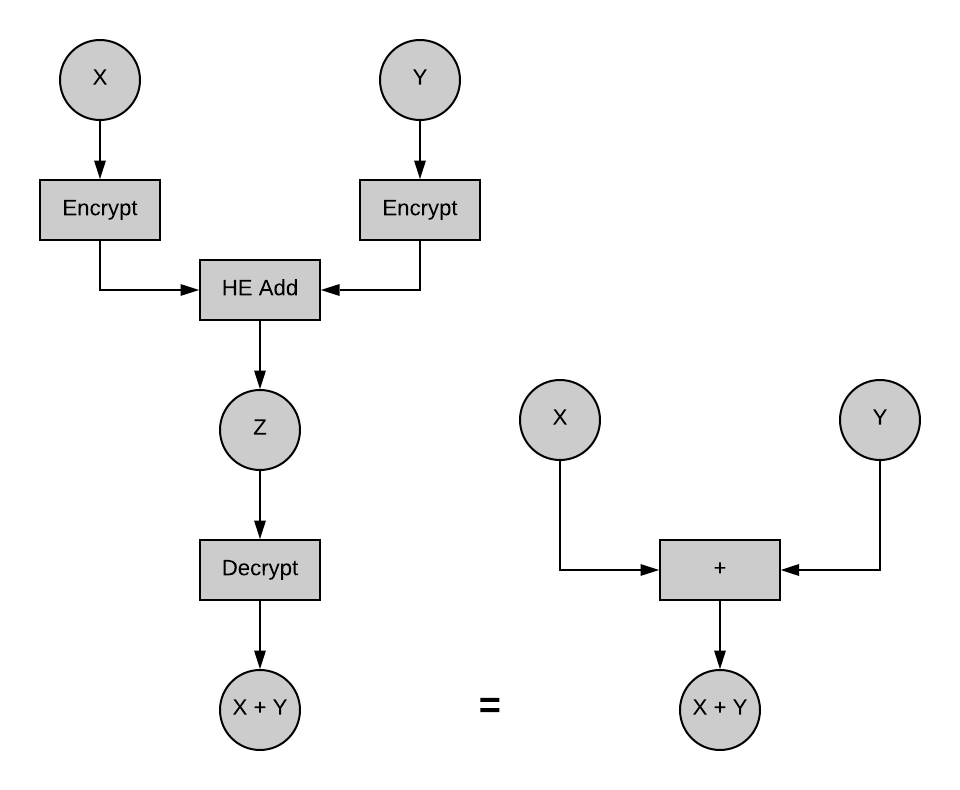
\includegraphics[scale=0.8]{Figuras/he-black-box.png}
    \caption{Comparativa de suma bajo esquema FHE y sin él \cite{tenseal2021}}
    \label{fig:fhe_img}
\end{figure}

\paragraph*{Differential Privacy}\mbox{}\\
%DP
La privacidad diferencial se entiende como una herramienta para cuantificar y limitar la fuga de información sensible sobre los participantes, de modo que pretende introducir cierto nivel de incertidumbre en el modelo, suficiente para enmascarar la contribución de cualquier usuario individual. La DP se cuantifica mediante los parámetros de pérdida de privacidad $(\epsilon, \delta)$, donde menor $(\epsilon, \delta)$ corresponde a mayor privacidad.

Normalmente en FL, el papel de coordinador es la parte confiada a implementar el mecanismo de DP en el sistema, asegurándose que sólo salidas 'privatizadas' del modelo son liberadas a terceros o al usuario final. Sin embargo, se puede reducir la necesidad de esta parte de confianza usando \textit{privacidad diferencial local}, si cada participante perturbase su propio modelo añadiendo ruido antes de la agregación de actualizaciones, por ejemplo.

\paragraph*{Zero Knowledge Proof}\mbox{}\\
%ZKP
Las pruebas de conocimiento cero son  unas técnicas criptográficas que permiten a un cliente probar a otro que ha ejecutado cierto computo o programa sobre unos datos según lo acordado, sin comprometer ni revelar ninguna información sensible sobre ella.

En el contexto de FL se puede usar para dos situaciones: el servidor podría demostrar que ha realizado ciertas operaciones específicas como la agregación o adición de ruido para DP y, por último, los clientes podrían demostrar al servidor que sus entradas y comportamiento han seguido la especificación o protocolo acordado.

\subsubsection{Casos de uso, \textit{software} y \textit{datasets}}
%Ejemplos de posibles aplicaciones, software de desarrollo y prd y datasets
Siendo un mecanismo que permite modelos de ML personalizados y compartidos, construidos sobre conjuntos de datos descentralizados y esparcidos entre múltiples participantes sin comprometer la privacidad y seguridad de estos tiene, por tanto, un futuro prometedor en numerosos ámbitos, como el financiero, sanitario, educativo, \textit{smart city} o \textit{edge computing}, incentivado por el número creciente de dispositivos móviles y embebidos conectados a internet (\textit{edge devices}, dentro del marco conocido como \textit{IoT}).

\vspace{1em}

En cuanto al \textit{software} disponible a día de hoy, en el ámbito de la investigación y simulación, algunas de las librerías más destacadas son:

\begin{itemize}[itemsep=2pt, topsep=2pt]
    \item \textit{TensorFlow Federated}: framework de código abierto de FL y otros cálculos con datos descentralizados para la investigación y experimentación simulada, en Python.
    \item \textit{PySyft}: biblioteca en Python de código abierto que añade seguridad y privacidad, desacoplando los datos del entrenamiento del modelo. De los creadores de TenSEAL.
    \item \textit{Flower}: framework que provee infraestructura para el aprendizaje y evaluación de algoritmos de FL, para los cuales es agnóstico, facilitando la implementación y el uso de diseños propios.
    \item \textit{PyVertical}: proyecto para la implementación de aprendizaje federado vertical (VFL) en Python, usando PySyft.
\end{itemize}

En cuanto a los conjuntos de datos para el entrenamiento de estos modelos, se tienen que simular conjuntos descentralizados, normalmente diseccionando reconocidos conjuntos centralizados.

\subsection{Algoritmos verdes}

La Inteligencia Artificial y, por tanto, el Aprendizaje Automático, no están exentos de traer consigo riesgos para el cambio climático derivados del coste energético asociado al desarrollo y aplicación de estas tecnologías. En este sentido, parece que jueguen roles opuestos ya que, por un lado, pueden colaborar como papel fundamental en la reducción de esta crisis{ }--{ }al diseñar redes eléctricas inteligentes (\textit{smart-grid}), desarrollando infraestructura sostenible o modelando nuevos sistemas climáticos{ }--{ }y, por otro, se están convirtiendo en un emisor de carbono cada vez más significante.

Por ejemplo, en el articulo '\textit{Energy and Policy Considerations for Deep Learning in NLP}' \cite{energy_ml}, de 2019, se cuantificaron los costes medioambientales y el $CO_2$ equivalente del entrenamiento de modelos avanzados de procesamiento de lenguaje natural (NLP), estimando que cada uno supuso alrededor de $300.000$ kg de dióxido de carbono, parejo a las emisiones producidas por 125 vuelos de ida y vuelta entre \textit{Nueva York} y \textit{Beijing}, para hacerse una idea.

Pero es que, además de esto, en el anterior estudio sólo se tuvieron en cuenta los costes de entrenamiento de dicho modelo basándose puramente en su demanda computacional aunque, una visión más acertada y global de este impacto, debería de considerar también el efecto de la infraestructura necesaria en torno al despliegue de estos sistemas por parte de las \textit{Big Tech}, así como el origen de la energía dispensada a estos. Este tema se tratará en más detalle en el apartado de emisiones y huella de carbono de la IA de esta misma sección.

Es por eso que, cada vez más, se está apostando por una concienciación para el desarrollo de la IA dentro de un contexto de responsabilidad, comprendiendo el impacto medioambiental que suponen y fomentando el desarrollo de una inteligencia artificial sostenible, que ponga en equilibrio \textit{eficiencia} y \textit{eficacia} y aplique buenas prácticas, marcando una distinción entre lo que algunos artículos ya denominan \textbf{Algoritmos Verdes} \cite{carbon_computation} o \textbf{Green \& Red AI} \cite{green_red_ai}.

En la última sección, para finalizar, hablaremos de algunas de las iniciativas políticas puestas en marcha a nivel europeo y nacional para fijar marcos de referencia, objetivos de desarrollo sostenible e integración en el tejido productivo de estas nuevas tecnologías.

En definitiva, es importante tener en cuenta que, aunque la IA es una herramienta con muchísimo potencial, también se puede convertir en una gran consumidora de recursos, por lo que hay que tener presente que los beneficios{ }--{ }progreso científico, tecnológico, social, etc.{ }--{ }de esta deberá siempre compensar sus inconvenientes.

\subsubsection{IA verde y roja}
\label{ss:green_ia}

Para asegurarse de que la IA sea beneficiosa también en el aspecto medioambiental es importante alentar a los investigadores a que prioricen el empleo y desarrollo de \textit{hardware} y algoritmos computacionalmente eficientes, así como estandarizar la publicación de informes de rendimiento que contengan resultados de tiempos de entrenamiento y susceptibilidad de los hiperparámetros del modelo.

Y es que, en un estudio realizado por \textit{Dario Amodei} \cite{openai_compute}, en 2018, se descubrió que los costes computacionales utilizados para el entrenamiento de grandes modelos de IA se vienen duplicando desde 2012 cada tres meses y medio aproximadamente, como se observa en la figura \ref{fig:moore_law}. De continuar esta tendencia, significaría un incremento incluso mayor que el observado en la clásica \textit{Ley de Moore} sobre el número de transistores en los circuitos integrados.

Otro artículo, titulado '\textit{Green AI}' \cite{green_red_ai}, ha acuñado el término \textbf{IA Verde} para describir la tendencia reciente de desarrollar el aprendizaje automático de manera sostenible, en contraste con lo que también denominan \textbf{IA Roja}.

En este estudio se hace un llamado a considerar la \textbf{eficiencia} como un criterio de igual importancia{ }--{ }al mismo nivel que las métricas de eficacia{ }--{ }en las investigaciones y desarrollos de ML. Además, propone la inclusión de un precio o coste financiero que refleje los gastos asociados al desarrollo y entrenamiento de estos modelos, premiando así el diseño y la eficiencia y no la fuerza bruta.

No por ello hay que restar importancia a los resultados obtenidos por dichos modelos, ya que contribuyen y llevan al extremo las fronteras conocidas de la IA, pero el retorno en las mejoras de rendimiento obtenidas se van a ver reducidas cada vez más, al tiempo que demandan mayores recursos.

\vspace{0.5em}

Existen tres factores determinantes para entender lo que se considera como \textbf{IA Roja}, que serían:
\begin{enumerate}[noitemsep]
    \item \textbf{E}: coste de ejecutar el modelo con una sola muestra.
    \item \textbf{D}: tamaño del \textit{dataset} o conjunto de datos.
    \item \textbf{H}: número de ajustes en hiperparámetros, es decir, cuantas veces el modelo es entrenado durante su desarrollo.
    \item[] \textbf{R}, coste de producción de un determinado resultado o rendimiento.
\end{enumerate}
\begin{equation}
    \text{Coste(}R\text{)} \propto E \cdot D \cdot H
\end{equation}

%todo figura
\begin{figure}[H]
    \centering
    \begin{subfigure}{.8\linewidth}
        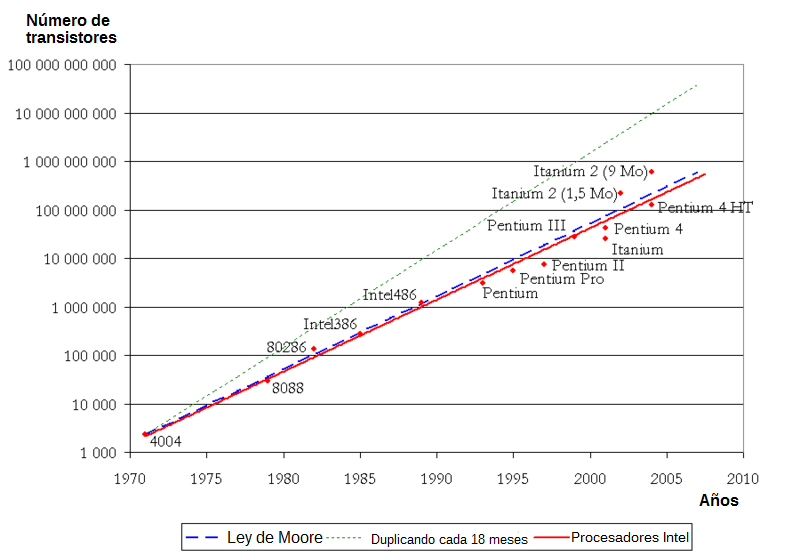
\includegraphics[width=\linewidth,height=.8\linewidth]{Figuras/moore_law_2.png}
        \caption{Ley de Moore comparada con datos históricos \cite{moore}}
    \end{subfigure}
    \vfill
    \begin{subfigure}{.8\linewidth}
        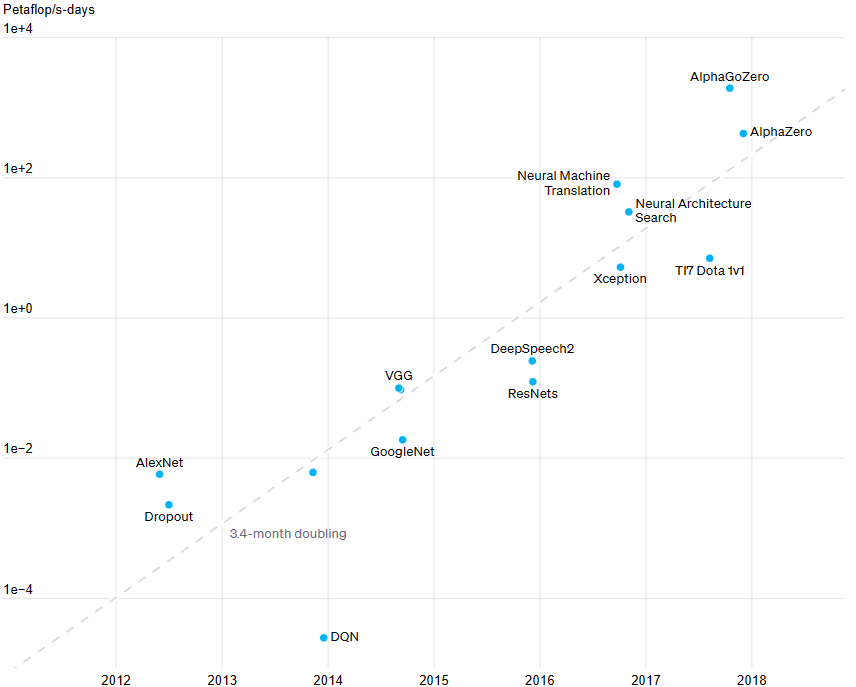
\includegraphics[width=\linewidth,height=.8\linewidth]{Figuras/moore_law_1.png}
        \caption[Coste computacional IA]{Coste computacional, en \textit{pfs-día} \protect\footnotemark[2], para el entrenamiento de distintas IA \cite{openai_compute}}    
    \end{subfigure}
    \caption[Ley de Moore vs IA]{Comparación entre ratios de crecimiento del número de transistores en circuitos integrados y costes computacionales en IA\protect\footnotemark[3]}
    \label{fig:moore_law}
\end{figure}
\footnotetext[2]{petaflop/s$\cdotp$día (\textit{pfs$\cdotp$día}) recordemos que los FLOPS son operaciones de coma flotante por segundo y el \textit{pfs$\cdotp$día} intenta dar una medida de consumo computacional semejante al kW$\cdotp$h para energía eléctrica.}
\footnotetext[3]{Advertir como ambos ejes verticales, para el número de transistores y de pfs$\cdotp$día, se encuentran en escala logarítmica.}

Cuando los costes de producir un resultado en un modelo de IA incrementan linealmente con alguno de los factores anteriores, estamos ante IA Roja. Contrariamente, definen la \textbf{IA Verde} como:
\begin{quote}
Investigación en inteligencia artificial que produzca nuevos resultados sin aumentar su coste computacional, e idealmente reduciéndolo.    
\end{quote}

En el citado artículo \cite{green_red_ai} también se dan una serie de recomendaciones en cuanto a métricas de eficiencia a utilizar en las investigaciones de IA, entre las cuales destacamos las siguientes:
\begin{itemize}[noitemsep]
    \item \textbf{Consumo eléctrico}
    \item \textbf{Tiempo de ejecución}
    \item \textbf{Número de parámetros}
    \item \textbf{FPO} (Floating Points Operations)
\end{itemize}
Las tres primeras métricas son agnósticas en cuanto a la fuente de energía utilizada pero dependientes del \textit{hardware} sobre el que se ejecute el modelo, por lo que puede ser difícil distinguir las contribuciones de un mejor diseño a las de una mejor maquina. Por ello el estudio se decanta por utilizar el \textbf{FPO}, es decir, el número de operaciones de coma flotante como estimación de la cantidad de trabajo realizado. Esta métrica está ligada directamente al consumo energético y al tiempo de ejecución, sin depender del \textit{hardware} subyacente.

\vspace{0.5em}

En la figura \ref{fig:eficiencia_ml} se puede observar esta tendencia en la disminución de la mejora de la exactitud con el sucesivo aumento de los costes computacionales.

\begin{figure}[H]
    \centering
    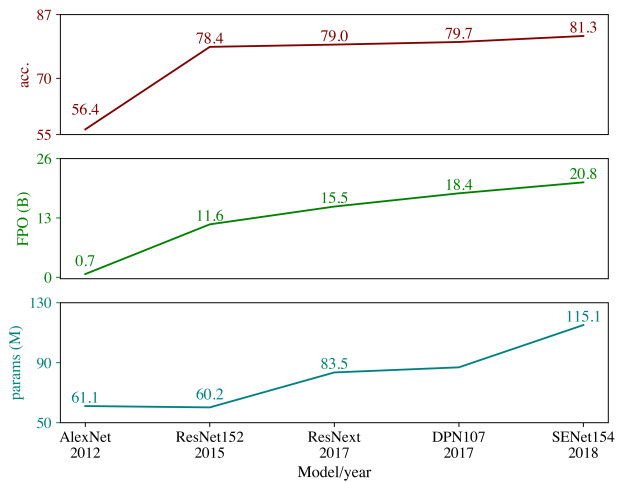
\includegraphics[scale=0.8]{Figuras/eficiencia_ml.png}
    \caption{Distintos modelos de detección de objetos en visión artificial: exactitud (acc) - FPO (billones) y  número de parámetros del modelo (millones) \cite{green_red_ai}}
    \label{fig:eficiencia_ml}
\end{figure}

No todos los problemas requieren soluciones basadas en el ML, y resolver problemas sencillos que pueden ser tratados con una IA menos intensiva computacionalmente, con redes neuronales profundas, por ejemplo, es un despilfarro.

\subsubsection{Emisiones y huella de carbono de la IA} \label{ss:emisiones_co2_ia}

Una métrica que no abordó el estudio anterior es el de las emisiones de carbono e impacto medioambiental, considerada fuera del alcance al depender estas de la infraestructura y fuentes de energía locales que abastezcan a los equipos, resultando inviable comparar investigaciones realizadas en lugares y épocas distintas.

Y es que, por ejemplo, en un dossier reciente publicado por el \textit{Electric Power Research Institute} (EPRI) \cite{epri_ai}, se da cuenta de como el consumo eléctrico de los centros de datos de las denominadas \textit{Big Tech} se ha doblado en el período 2017-2021, y como esperan llegar a suponer hasta el 9.1\% del consumo eléctrico total de Estados Unidos para el año 2030, comparado con el 4\% estimado a fecha de 2024. Además, esta demanda energética se halla geográficamente concentrada, lo cual complica todavía más la carga eléctrica que deben soportar estas redes. Este aumento viene impulsado por la adopción masiva de los modelos generativos de IA, por ejemplo \textit{ChatGPT}, del cual estima dicho estudio requerir 2.9 W$\cdotp$h por consulta, diez veces más que una búsqueda en \textit{Google}, con 0.3 W$\cdotp$h.

Y no es solo el consumo energético; en recientes publicaciones \cite{water_ai}, se da cuenta del grandísimo consumo de agua requerido por estos \textit{data centers}. Así, el entrenamiento del modelo \textit{GPT-3} requirió de 700.000 litros de agua corriente para refrigerar los equipos de estos centros de datos. Estiman, además, que la demanda global de IA para 2027 requerirá de unos 5000 millones de $m^3$ de agua, que, en comparación, supone la mitad de la consumida anualmente en todo Reino Unido.

Es por ello que cada vez aparecen más herramientas para contabilizar estos aspectos, como las presentadas a continuación. En ambas se trabajan formas de cuantificar las emisiones de carbono teniendo en cuenta la ubicación de la maquina que ejecuta el entrenamiento del modelo, su duración, el tipo de energía que usa y el \textit{hardware} en el que se realiza. La primera es una especie de simulador web y la segunda herramienta se puede integrar fácilmente dentro del propio código del modelo.

\paragraph*{Cálculo y simuladores}\mbox{}\\
En el estudio '\textit{Green Algorithms: Quantifying the carbon footprint of computation}' \cite{carbon_computation}, realizaron un simulador web para calcular estas emisiones, llamado \href{http://calculator.green-algorithms.org/}{Green Algorithms}, como se observa en la figura \ref{fig:ml_calc_carbon_ml}:

\begin{figure}[h!]
    \centering
    \begin{subfigure}{.55\linewidth}
        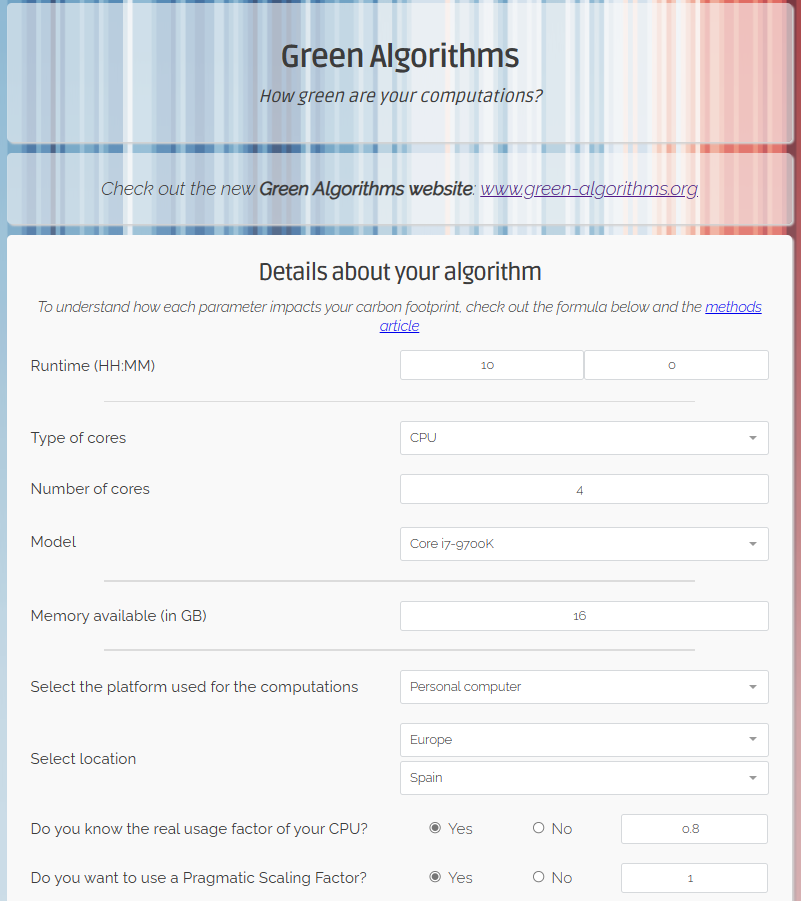
\includegraphics[width=\linewidth]{Figuras/ml_calc_3.png}
        \caption{Parámetros de la herramienta}
    \end{subfigure}
    \vfill
    \begin{subfigure}{.55\linewidth}
        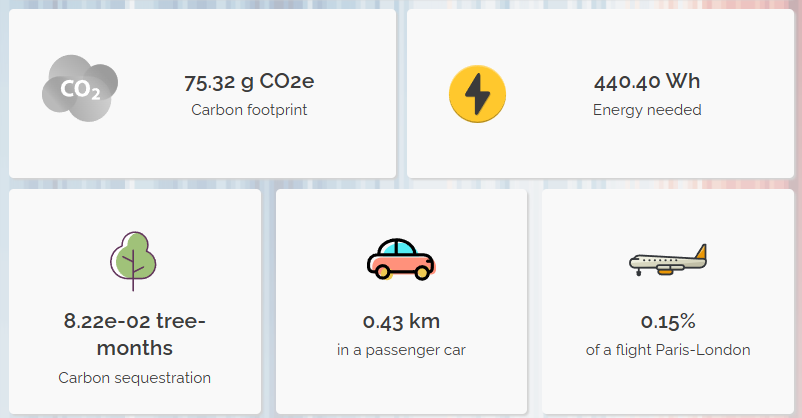
\includegraphics[width=\linewidth]{Figuras/ml_calc_4.png}
        \caption{Resultados de la herramienta}
    \end{subfigure}
    \caption{Simulador web para la estimación del cálculo de $CO_2$ equivalente de una RNA \cite{carbon_computation}}
    \label{fig:ml_calc_carbon_ml}
\end{figure}

Los cálculos realizados para producir esas estimaciones se computan así:

\begin{equation}
\label{eq:4}
    E = t \cdot (\eta_c \cdot P_c \cdot \mu_c + \eta_m \cdot P_m) \cdot PUE \cdot 0.001
\end{equation}

Donde, en \eqref{eq:4}, $t$ es el tiempo de ejecución en horas, $\eta_c$ el número de núcleos del CPU, 
$\eta_m$ el tamaño de la memoria RAM disponible en GB, $\mu_c$ es el factor de uso del CPU, $P_c$ la potencia requerida por cada uno de los núcleos en W, $P_m$ la potencia requerida por la memoria en W y, por último, $PUE$ (\textit{Power Usage Effectiveness}) la eficiencia del centro de datos, medida como la razón entre la potencia o energía requerida total dividido entre la destinada al uso del equipamiento TI.

Por último, la estimación de la huella de carbono ($g\,CO_{2}^{eq}$) la hacen multiplicando la energía precisada en \eqref{eq:4} ($kW \cdotp h$) multiplicada por el $CI$, \textit{carbon intensity} ($\frac{gCO_{2}^{eq}}{kW \cdotp h}$), de la localización:
\begin{equation}
\label{eq:5}
    C = E \cdot CI
\end{equation}

Por otro lado, el equipo de \href{https://codecarbon.io}{\textit{CodeCarbon}} presenta un planteamiento muy similar al anterior, con la diferencia de que han desarrollado una librería en Python que se puede integrar en cualquier algoritmo desarrollado con este lenguaje de programación y que, monitorizando directamente los recursos disponibles y el \textit{hardware} de la maquina, realiza las estimaciones de las ecuaciones \eqref{eq:4} y \eqref{eq:5} automáticamente, generando los informes correspondientes, como los que se aprecian en la figura \ref{fig:codecarbon_img_dash}.

\begin{figure}[h!]
    \centering
    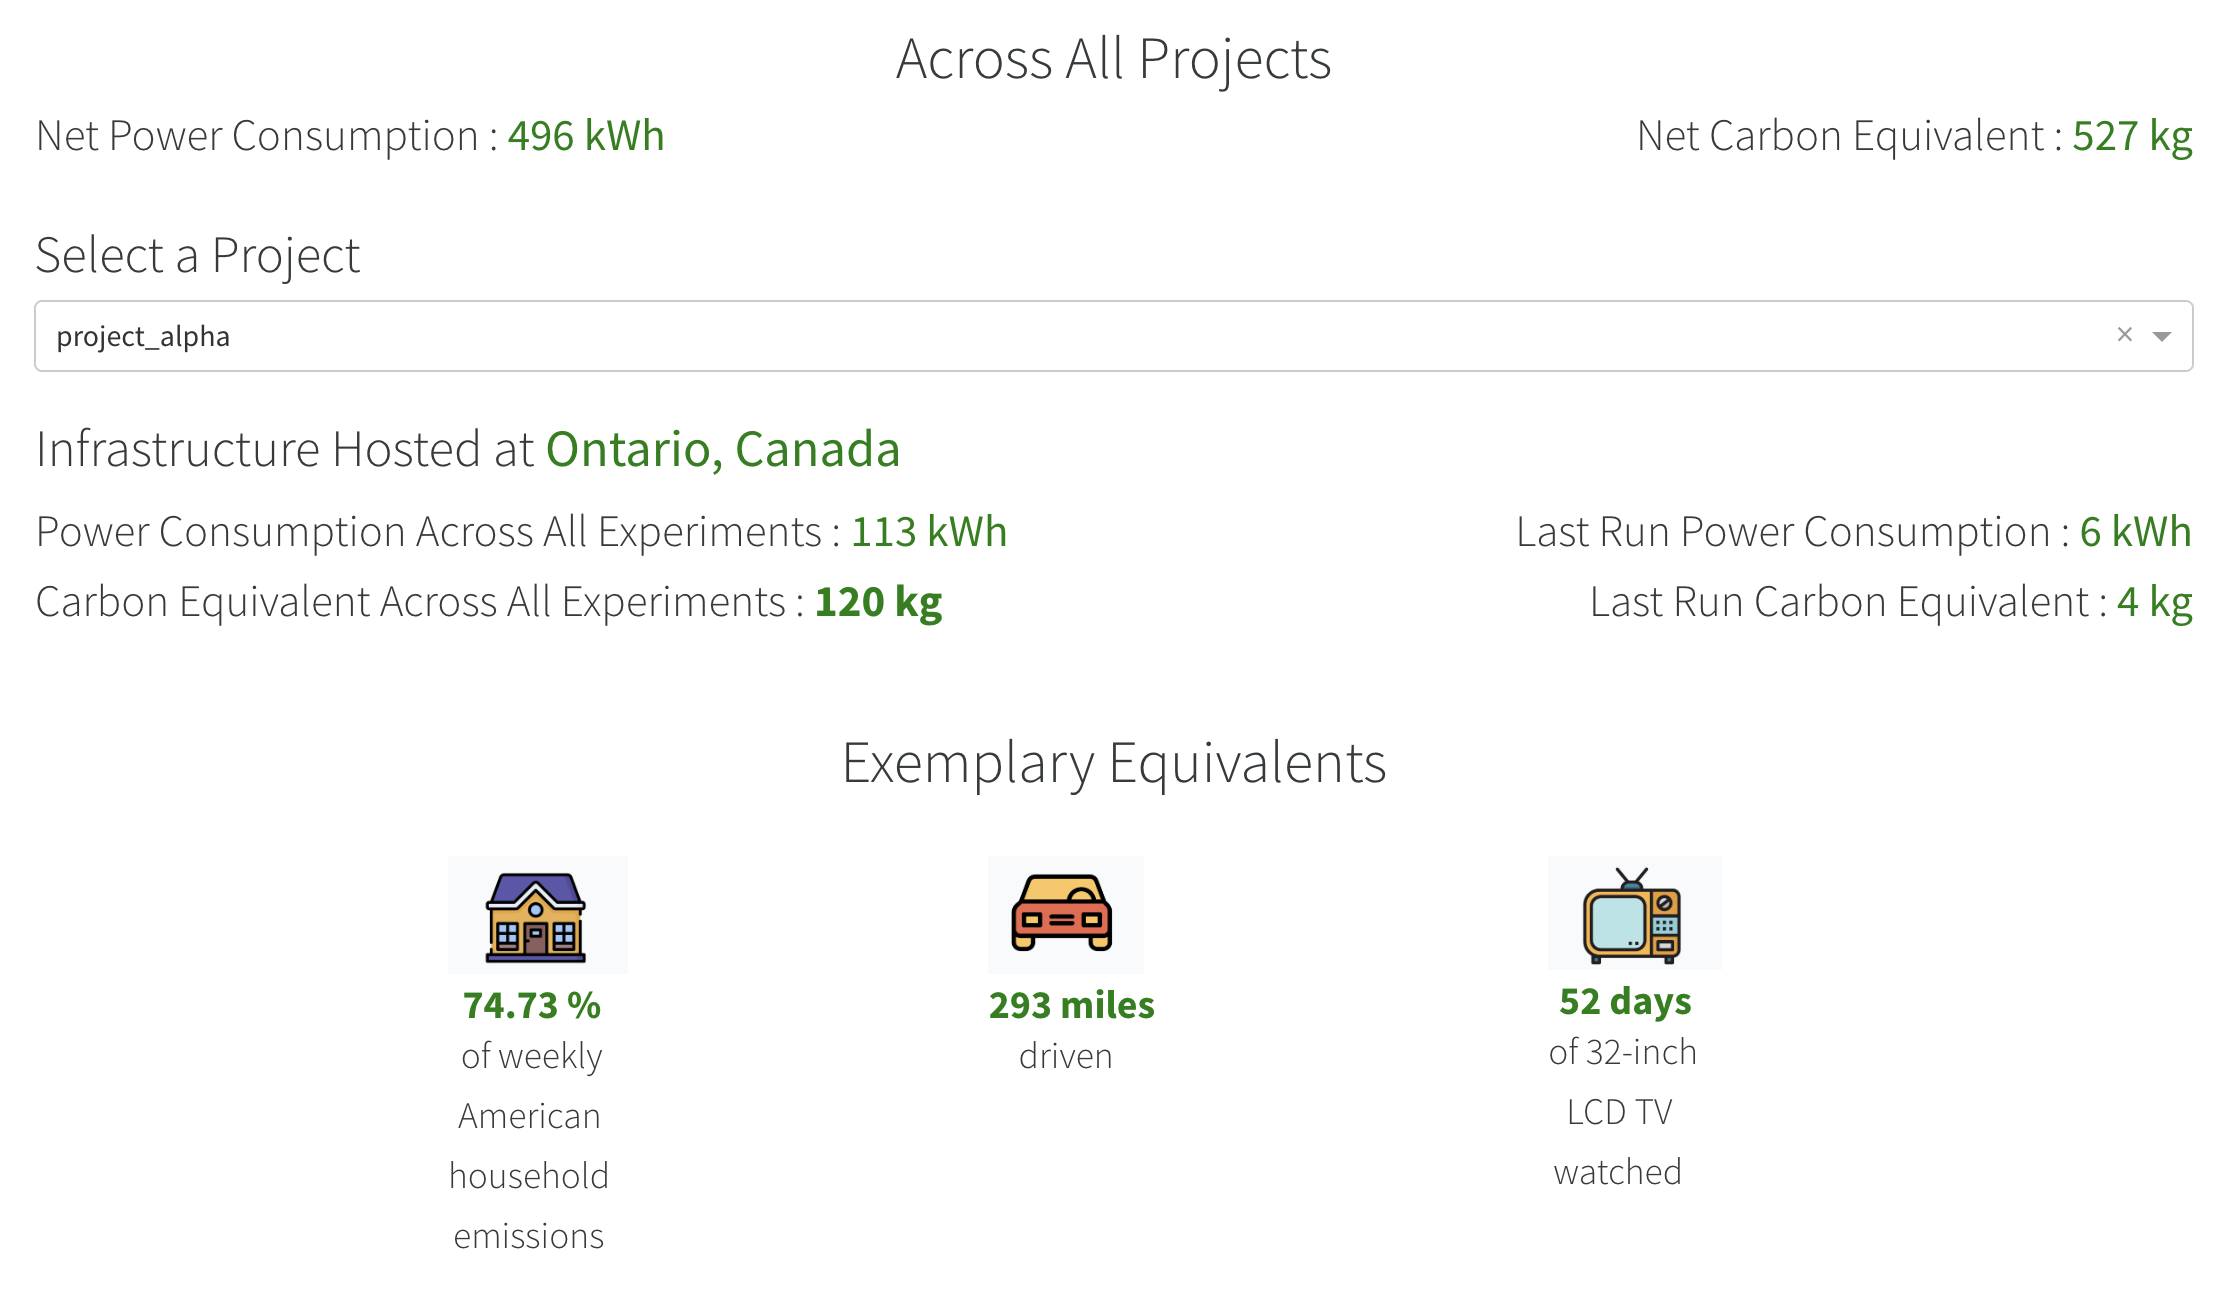
\includegraphics[scale=0.4]{Figuras/codecarbon_dash.png}
    \caption{Informe generado por la herramienta CodeCarbon \cite{codecarbon}}
    \label{fig:codecarbon_img_dash}
\end{figure}

\subsubsection{Iniciativas políticas europeas y nacionales}
\label{ss:politica_ia}
%ENIA, PNAV y EGD
Existe cada vez mayor interés, por parte de entidades gubernamentales a nivel europeo y nacional, de introducir marcos regulatorios, buenas prácticas y fomentar el desarrollo sostenible en temas relacionados con la computación de altas prestaciones como la IA u otras tecnologías intensivas tipo \textit{blockchain} como respuesta al conflicto climático, reconociéndolas como fuentes de emisiones en cuanto atañe a las tecnologías de la información.

Así tenemos, por ejemplo, el amplio estudio promocionado por la Comisión Europea \textit{'The role of Artificial Intelligence in the European Green Deal'} \cite{libro_EGD}, donde se exponen una serie de recomendaciones para equilibrar un buen uso de estas herramientas con su impacto medioambiental e integrarlos en las cadenas de valor y tejido industrial. Respecto a la ejecución de algoritmos, la UE está estudiando también mejores prácticas para instaurar un mercado de tecnologías de computación en la nube respetuosas con el medioambiente.\footnotemark[1]

\footnotetext[1]{\href{https://ec.europa.eu/newsroom/dae/document.cfm?doc_id=71330}{\textit{Energy-efficient Cloud Computing 
Technologies and Policies for an 
Eco-friendly Cloud Market}}}

En el panorama nacional existen dos iniciativas que surgen del \textit{Ministerio de Asuntos Económicos y Transformación Digital}, en concreto de la \textit{Agenda España Digital 2026}, que son el ENIA \cite{libro_ENIA}{ }--{ }\textit{Estrategia Nacional de Inteligencia Artificial}{ }--{ }y el PNAV \cite{libro_PNAV}{ }--{ }\textit{Programa Nacional de Algoritmos Verdes}{ }--{}, esta última incluida como expansión de uno de los ejes estratégicos de la primera, y cuyos puntos clave y objetivos desarrollamos a continuación:

\begin{enumerate}[noitemsep, topsep=5pt]
    \item \textbf{Fomentar la investigación en materia de inteligencia artificial verde}, a través de financiación pública.
    \item \textbf{Promover el uso de infraestructuras y servicios eficientes}, apoyando el desarrollo de estándares y herramientas para la medición del consumo de estos algoritmos e incentivando el consumo energético renovable y sostenible de los centros de datos que los ejecuten.
    \item \textbf{Integrar la inteligencia artificial verde y Blockchain en el tejido productivo}, creando nuevos mercados económicos.
    \item \textbf{Dinamizar el mercado español a través de la inteligencia artificial verde}, promocionando su adopción en sectores que contribuyan al cambio climático.
\end{enumerate}

\subsubsection{Notación Big-O}
Una herramienta esencial a la hora de describir la complejidad computacional de un algoritmo es la llamada Notación Big-O, conocida también como notación \textit{Asintótica} o \textit{Landau}, en honor a uno de los autores a los que se atribuye, Edmund Landau, matemático alemán de comienzos del siglo pasado.

La Notación Big-O se usa para medir como de bien \textbf{escala} un algoritmo o programa{ }--{ }según aumenta el número de elementos procesados{ }--{ }respecto al tiempo que tarda en ejecutarlo, es decir, nos da el \textit{ratio de crecimiento} de dichas operaciones.

Es una medida muy útil para comparar la \textbf{eficiencia} entre algoritmos, ya que aunque no nos proporcione el tiempo de ejecución exacto de estos, sí nos da una idea de cómo de rápido se incrementa este tiempo de ejecución en función del número de datos de entrada. Así, se clasifican los algoritmos según la clase de ratio de crecimiento que tengan, una medida de su buena/mala escalabilidad.

En la tabla \ref{tbl:bigo} se resumen algunas de estas clases de notaciones y sus nombres, y en la figura \ref{fig:bigo} se puede observar gráficamente la representación de estas, enfrentando el número de pasos o operaciones requeridas por el algoritmo frente al número de elementos.

%tabla
\begin{table}[htb]
    \centering
    \begin{tabular}{@{}ll@{}}
    \toprule
    Notación            & Nombre             \\ \midrule
    $O(1)$              & constante          \\
    $O(\log n)$         & logarítmico        \\
    $O(n)$              & lineal             \\
    $O(n \cdot \log n)$ & lineal logarítmico \\
    $O(n^2)$            & cuadrático         \\
    $O(2^n)$            & exponencial        \\
    $O(n!)$             & factorial          \\ \bottomrule
    \end{tabular}
    \caption{Órdenes más utilizados en análisis de algoritmos para la notación Big-O}
    \label{tbl:bigo}
\end{table}

\begin{figure}[htb]
    \centering
    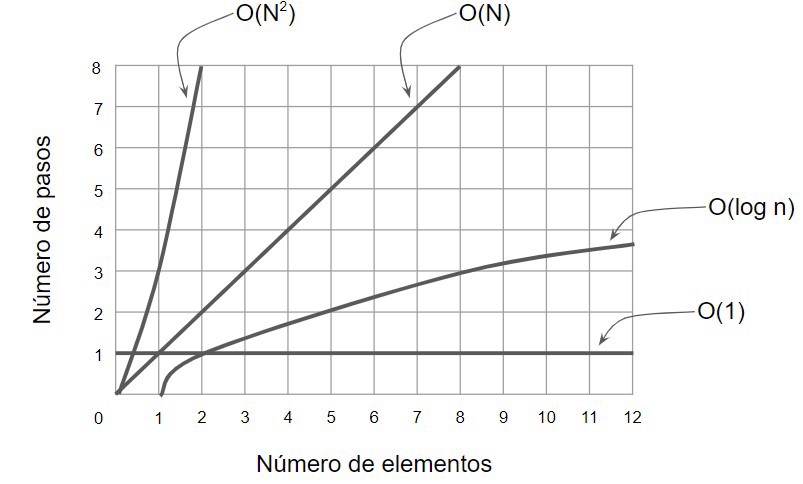
\includegraphics[scale=0.6]{Figuras/bigo.jpg}
    \caption{Gráfica del ratio de crecimiento y escalabilidad de las distintas clases de notaciones Big-O \cite{bigo}}
    \label{fig:bigo}
\end{figure}

Mayor número de operaciones representa mayor tiempo de ejecución y mayor coste computacional, lo cual implica un mayor coste energético y por lo tanto una \textbf{menor eficiencia energética}.

\vspace{1em}

Veamos, con un ejemplo, las tres propiedades que se suelen asumir a la hora de analizar el grado $O$ de una función $f(n)$:

\begin{enumerate}
    \item Si una función o algoritmo se puede escribir como una suma finita de otras funciones, entonces marca el grado de $f(n)$ la que tenga mayor ratio de crecimiento.
    \item Si una función o algoritmo es multiplicada por algún factor contante, es decir, uno que no dependa de $n$, se puede omitir.
    \item Si un algoritmo es producto de dos funciones el grado resultante del mismo es el producto de ambos.
    \begin{equation}
        f_1 = O(g_1) \quad f_2 = O(g_2) \rightarrow f_1 f_2 = O(g_1 g_2)
    \end{equation}
\end{enumerate}

Dadas las anteriores características, es fácil demostrar que, para el siguiente ejemplo \eqref{eq:bigo}, el grado de complejidad de la función es cúbico:

\begin{equation}
    \label{eq:bigo}
    f(n) = 5 \log n + 5 (\log n )^4 + 2n^2 + n^3 = O(n^3)
\end{equation}

Asegurarse de que los algoritmos de optimización presentes en los modelos usados en FL sean lo más eficientes posibles implica un análisis de este tipo para saber como se comporta ante distintos volúmenes de datos de entrada, y saber así como de bien escala. Obviamente es preferible algoritmos de ordenes bajos, como lineal o logarítmico, pero eso dependerá únicamente del modelo y las técnicas de optimización empleadas.

\vspace{1em}

Existe, sin embargo, una razón por la que el aprendizaje federado se beneficia y gana mayor eficiencia que sus contrapartidas tradicionales, aún usado modelos y algoritmos de optimización equivalentes, y que se pueden explicar usando esta notación:

\begin{enumerate}[itemsep=5pt]
    \item Sea un modelo de ML $\mathcal{M}$ cuya fase de entrenamiento $\mathcal{E}$ implica un cuello de botella en su proceso de optimización marcado por el uso de cierto algoritmo de optimización $\mathcal{A}$ clasificado como de tiempo cuadrático $O(n^2)$.
    \item Sea $\theta$ el nº de operaciones, $\tau$ el tiempo de ejecución y  $\epsilon$ el coste energético, de modo que: 
    \item[] \begin{center}$\uparrow \theta \rightarrow \uparrow \tau \leadsto \uparrow \epsilon$ \end{center}
    \item Si el volumen de datos de entrada para cada ronda de $\mathcal{E}$ es de $\eta$, esto implica que: \begin{center}$\mathcal{A}_{ML}(\eta) \leadsto O(\eta^2) \implies \theta_{ML}$\end{center}
    \item Si este mismo volumen es distribuido entre múltiples participantes{ }--{ }p.ej. \textbf{cuatro}{ }--{ }de una red federada, las fases de $\mathcal{E}_{local}$ se benefician de una reducción inmensa en sus tiempos de ejecución y coste energético:
    \begin{equation}
        \mathcal{A}_{fed}(\eta) = \mathcal{A}_{local}(\frac{\eta}{4}) \cdot 4_\textit{clientes}  \leadsto O((\frac{\eta}{4})^2) \cdot 4_\textit{clientes} \implies \frac{\theta}{4} \rightarrow \frac{\tau}{4} \rightarrow \frac{\epsilon}{4} 
    \end{equation}
    \item Es decir, una reducción de tres cuartos en el tiempo, coste y construcción del modelo, siempre que supongamos condiciones ideales y una distribución perfectamente paralela y síncrona de clientes con igual poder computacional.
\end{enumerate}

He aquí uno de los grandes beneficios de estas técnicas de \textbf{FL}. Aún suponiendo participantes heterogéneos, con distintas potencias computacionales, y siendo estas, por separado, ínfimas en comparación a la que pueda tener una máquina o servidor de un gran centro de datos, se pueden encontrar beneficios derivados de su diseño distribuido tanto por tiempos de entrenamiento como en eficiencia energética, debido a que cada cliente entrena un modelo con los datos locales disponibles que luego se agregan en un modelo global.

\newpage

\section{Diseño e implementación}
En este capítulo se describe el diseño e implementación del sistema informático sobre el que se realizarán las pruebas de los distintos métodos desarrollados. Empezaremos con una vista global del conjunto y de su arquitectura, para luego describir en detalle los dispositivos embebidos, sistemas operativos, lenguajes de programación y librerías empleadas.

\subsection{Vista global del sistema}

Contamos con cinco dispositivos físicos a nuestra disposición para el desarrollo de las pruebas e investigación: dos ordenadores portátiles, dos modelos diferentes de Raspberry Pi y una Jetson Nano.

La división de trabajo y almacenamiento de datos se hará acorde a los límites y características de cada uno de ellos. Por esta razón los portátiles, al tener mayor capacidad, serán los encargados de albergar el servidor así como sucesivos lotes de clientes simulados, cuando realicemos las pruebas de escalabilidad.

El método desarrollado es una aplicación de un sistema de aprendizaje automático federado, en donde la computación y entrenamiento del modelo se hace de manera distribuida. Así, se conforma una red compuesta de varios dispositivos interconectados, siendo uno de ellos coordinador del proceso global, rol asignado al ordenador portátil más potente, trabajando en conjunto. También se han realizado pruebas, por comparativa, con algoritmos y técnicas equivalentes con arquitectura centralizada, llevadas a cabo de igual modo en dicho portátil.

\subsubsection*{Arquitecturas}
El diseño de estos sistemas se suele hacer siguiendo una arquitectura \textbf{cliente-servidor} clásica, donde un servidor orquestará el proceso de selección, entrenamiento, agregación y validación del modelo, y unos clientes que, teniendo acceso cada uno a su propio conjunto de datos, entrenarán un modelo local y recibirán las actualizaciones y directrices necesarias cuando sean llamados. Existen otro tipo de arquitecturas federadas, como, por ejemplo, las \textit{Peer-To-Peer} (P2P), que no hemos cubierto en este trabajo debido a que no ha sido la empleada en nuestro modelo. A continuación detallamos el funcionamiento de la arquitectura escogida:

\paragraph*{Cliente-Servidor}

Este tipo de arquitectura es la más utilizada en sistemas federados, conocida también como diseño tipo \textit{master-worker}. En ella, \textit{K} participantes o clientes, cada uno con un subconjunto del grupo de datos, entrenan de manera colaborativa el modelo de aprendizaje automático con la ayuda de un servidor{ }--{ }también denominado coordinador o servidor de agregación{ }--{}. Los supuestos para estos casos es que los participantes son honestos mientras que el servidor es honesto pero curioso (\textit{honest-but-curious}). Este concepto implica que, aunque el servidor no altere maliciosamente los resultados o cómputos del proceso, el diseño del algoritmo de entrenamiento tiene que prevenir cualquier tipo de fuga de información útil que este pueda recibir de los clientes.

\vspace{1em}

El proceso de entrenamiento de estos sistemas consiste normalmente de los siguientes pasos.

\begin{enumerate}[noitemsep]
    \item Los clientes entrenan localmente sus modelos y enmascaran sus resultados{ }--{ }p.ej. gradientes{ }--{ }mediante técnicas criptográficas o privacidad diferencial, para luego enviarlos de vuelta al servidor.
    \item El servidor recopila los resultados y realiza su agregación.
    \item El servidor envía de vuelta los resultados agregados a los participantes.
    \item Los clientes actualizan sus respectivos modelos locales con los resultados recibidos desencriptados.
\end{enumerate}

%figura cliente-servidor
\begin{figure}[htb]
    \centering
    %\includesvg[pretex=\tiny]{Figuras/diagrama_cliente_servidor.svg}
    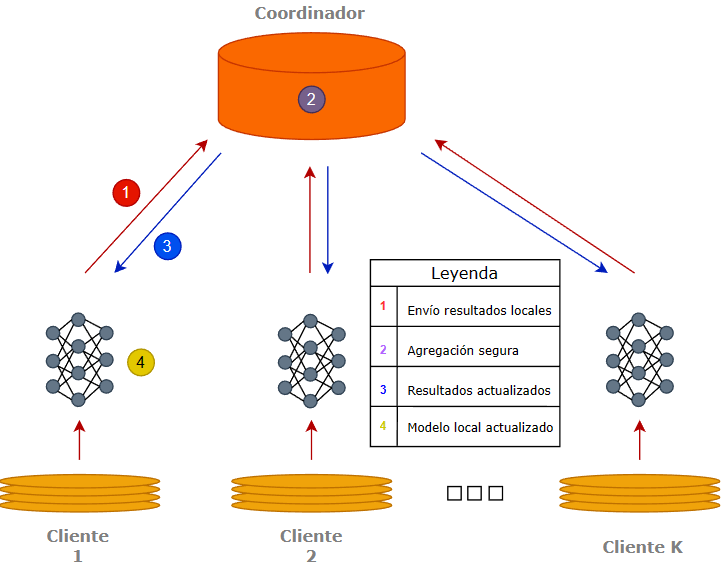
\includegraphics[scale=0.8]{Figuras/diagrama_cliente_servidor.png}
    \caption{Ejemplo de arquitectura cliente-servidor para sistema federado}
    \label{fig:arquitectura_cliente_servidor}
\end{figure}

En el caso de tratarse de un algoritmo iterativo, el proceso anterior se repite hasta que la función objetivo (\textit{loss function}) converja o se alcance el número máximo de rondas posibles.

\subsection{Sistemas informáticos}\label{sec:sist_infor}

Introducimos brevemente las especificaciones técnicas de los dispositivos físicos utilizados en el trabajo.

\subsubsection*{Sistemas embebidos}
Se denominan así a los sistemas de computación basados en microprocesadores o microcontroladores que están diseñados para realizar unas pocas funciones dedicadas y limitadas; en contraste con los ordenadores personales, de propósito general.

\paragraph*{Raspberry Pi}

Son una serie de computadoras de placa única (\textit{SBC}), de bajo coste y tamaño reducido, creadas en el Reino Unido por la \textit{Raspberry Pi Foundation} para fomentar el aprendizaje de informática y electrónica. Lanzada en 2012, ha evolucionado con sucesivas versiones, cada una con diferentes especificaciones. Estas placas se utilizan en proyectos variados como domótica, servidores web, centros multimedia, robótica y todo el ámbito del \textit{IoT}.

Todas sus versiones incluyen un procesador Broadcom, memoria RAM, puertos USB, HDMI, GPU, Ethernet, 40 pines GPIO, conector para cámara y ranura para tarjetas SD, lo que permite ejecutar sistemas operativos y aplicaciones de software. Su sistema operativo oficial es \textit{Raspberry Pi OS}, basado en Debian, aunque también es compatible con otros SO basados en arquitectura ARM.

\begin{figure}[h]
    \centering
    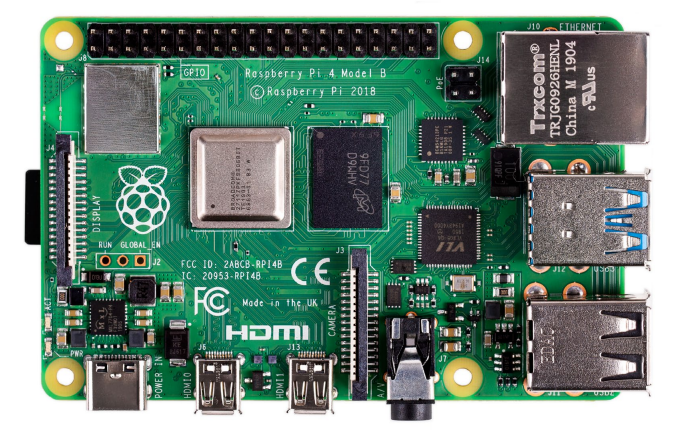
\includegraphics[width=0.7\textwidth]{Figuras/raspberry-modelo-producto.png}
    \caption{Raspberry Pi Model 4B}
    \label{fig:foto_raspberry_pi_4b}
\end{figure}

En la figura \ref{fig:foto_raspberry_pi_4b} se puede apreciar el aspecto de uno de estos modelos, el denominado Raspberry Pi Model 4B. Junto con otro, más pequeño y de menor rendimiento, llamado Raspberry Pi Zero W, que se puede observar en la figura \ref{fig:foto_raspberry_pi_zero}, son los dos dispositivos embebidos de este fabricante que emplearemos en este Trabajo Final de Grado.

\begin{figure}[h]
    \centering
    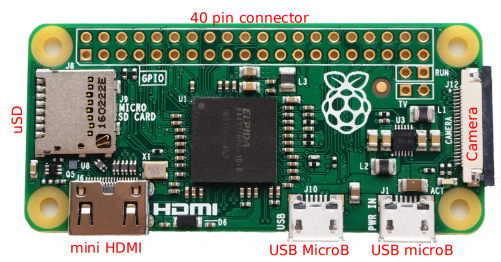
\includegraphics[width=0.7\textwidth]{Figuras/raspberry_foto_modelo.png}
    \caption{Raspberry Pi Zero W}
    \label{fig:foto_raspberry_pi_zero}
\end{figure}

En las tablas \ref{tab:especificaciones_raspberry_4b} y \ref{tab:especificaciones_raspberry_zerow} presentamos las especificaciones de cada uno de ellos:

\vspace{3cm}

\begin{table}[h]
    \flushleft
\begin{tabular}{ll}
\hline
\textbf{Procesador}    & Broadcom BCM2711 quad-core Cortex-A72 (ARM) @ 1.5GHz             \\
\textbf{Memoria}       & 1GB/2GB/4GB/8GB LPDDR4 (dependiendo del modelo).                  \\
\textbf{Conectividad}  & Wireless LAN. Bluetooth 5.0. BLE. Gigabit Ethernet. 4×USB.         \\
\textbf{GPIO}          & Encabezado GPIO estándar de 40-pines.                             \\
\textbf{Video y Audio} & 2×microHDMI. MIPI DSI. MIPI CSI. \\
\textbf{Multimedia}    & VideoCore VI @ 500 MHz GPU. Gráficos OpenGL ES 3.0.   \\
\textbf{Tarjetas SD}   & Ranura para MicroSD para SO y almacenamiento.                     \\
\textbf{Alimentación}  & 5V DC via USB-C. 5V DC via GPIO. PoE (requiere PoE HAT).          \\
\textbf{Entorno}       & Temperatura de funcionamiento 0-50ºC. \\ \hline
\end{tabular}
    \caption{Especificaciones de la Raspberry Pi Model 4B}
    \label{tab:especificaciones_raspberry_4b}
\end{table}


\begin{table}[h]
    \flushleft
    \begin{tabular}{ll}
\hline
\textbf{Procesador}    & ARM 11 Broadcom BCM2835 single-core CPU @ 1GHz  \\
\textbf{Memoria}       & 512MB RAM.                                      \\
\textbf{Conectividad}  & Wireless LAN. Bluetooth 4.1. BLE. 2×microUSB.   \\
\textbf{GPIO}          & Encabezado GPIO estándar de 40-pines.           \\
\textbf{Video y Audio} & miniHDMI. MIPI CSI.                             \\
\textbf{Multimedia}    & VideoCore IV  @ 400MHz GPU. Gráficos OpenGL ES 2.0. \\
\textbf{Tarjetas SD}   & Ranura para microSD para SO y almacenamiento.   \\
\textbf{Alimentación}  & 5V DC via microUSB. 5V DC via GPIO.             \\ 
\textbf{Entorno}       & Temperatura de funcionamiento 0-50ºC.  \\
    \hline
\end{tabular}
    \caption{Especificaciones de la Raspberry Pi Model Zero W}
    \label{tab:especificaciones_raspberry_zerow}
\end{table}

\paragraph*{Jetson Nano}

Son una serie de dispositivos embebidos de la compañía Nvidia que están diseñados específicamente para aplicaciones de IA y robótica. Sus modelos son pequeños, de bajo consumo y ofrecen un alto rendimiento para las tareas de procesamiento de datos intensivas de estos campos, como procesamiento de imágenes, detección de objetos, reconocimiento de voz o aprendizaje profundo. Se ofrecen diversos modelos, que vienen equipados con un amplio rango de potentes procesadores CPU/GPU, incluyendo además interfaces para cámaras, sensores y otros dispositivos externos.

En este Trabajo Final de Grado se ha utilizado el modelo Jetson Nano B01, del que se puede apreciar su aspecto en la figura \ref{fig:foto_jetson_nano} y sus especificaciones en la tabla \ref{tab:especificaciones_jetson_nano}.

\begin{figure}[h]
    \centering
    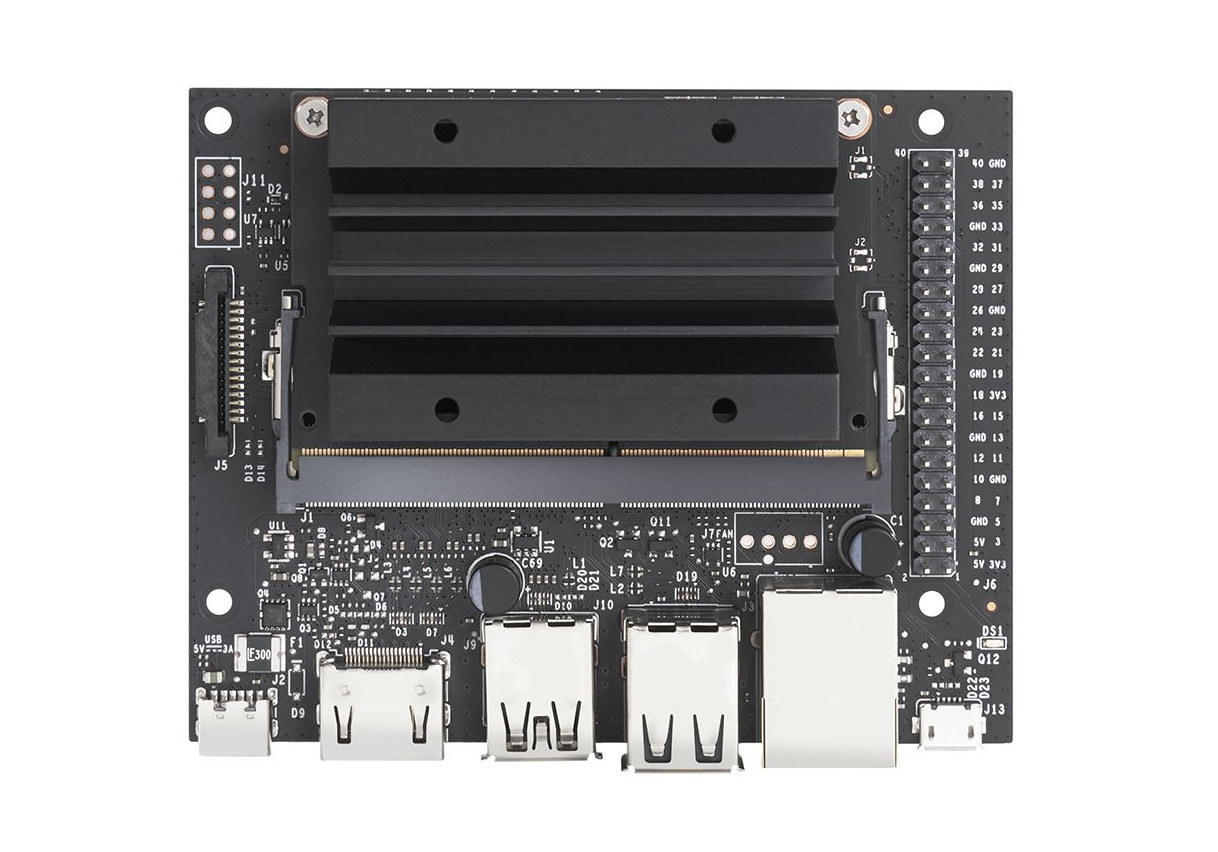
\includegraphics[width=0.7\textwidth]{Figuras/jetson_nano_foto_modelo.jpg}
    \caption{Jetson Nano}
    \label{fig:foto_jetson_nano}
\end{figure}

\begin{table}[H]
    \flushleft
    \begin{tabular}{ll}
\hline
\textbf{Procesador}    & Quad-core Arm A57 processor @ 1.43 GHz.                                    \\
\textbf{Memoria}       & 4GB LPDDR4 RAM.                                                            \\
\textbf{Conectividad}  & Ethernet. 4×USB. 1×microUSB.                                               \\
\textbf{GPIO}          & 260-pin SO-DIMM. Puertos expansión GPIO 40-pines. \\
\textbf{Video y Audio} & HDMI. eDP 1.4. 4×MIPI CSI.                                                 \\
\textbf{Multimedia}    & 128-core Maxwell GPU.                                                      \\
\textbf{Tarjetas SD}   & Ranura para microSD para SO y almacenamiento.                              \\
\textbf{Alimentación}  & 5V/4A DC via cable. 5V/2A via microUSB. PoE.                               \\
\textbf{Entorno}       & Temperatura de funcionamiento -25/80ºC.  
                            \\ \hline
\end{tabular}
    \caption{Especificaciones de la Jetson Nano}
    \label{tab:especificaciones_jetson_nano}
\end{table}

\subsubsection*{Sistemas físicos y simulados}

Los ordenadores portátiles son Lenovo, modelos Legion Y540-15IRH y ThinkPad X200, cuyo aspecto y especificaciones se pueden observar en la figura \ref{fig:foto_lenovo_modelo} y en las tablas \ref{tab:especificaciones_lenovo} y \ref{tab:especificaciones_x200}, respectivamente.

\begin{figure}[h]
    \centering
	\begin{subfigure}{.45\linewidth}
		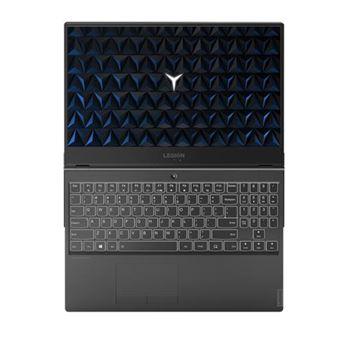
\includegraphics[width=.9\linewidth]{Figuras/foto_lenovo.jpg}
		\caption{Lenovo Legion Y540}
	\end{subfigure}
	\begin{subfigure}{.45\linewidth}
		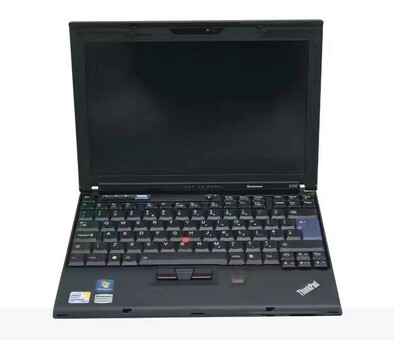
\includegraphics[width=.9\linewidth]{Figuras/lenovo_x200.jpg}
		\caption{Lenovo ThinkPad X200}
	\end{subfigure}
    \caption{Ordenadores portátiles disponibles}
    \label{fig:foto_lenovo_modelo}
\end{figure}

\begin{table}[]
    \flushleft
\begin{tabular}{ll}
\hline
\textbf{Procesador}     & Intel(R) Core(TM) i7-9750H CPU @ 2.60GHz  \\
\textbf{Memoria}        & 16GB RAM.                                 \\
\textbf{Conectividad}   & Ethernet. Wireless LAN. Bluetooth. 3×USB. \\
\textbf{Video y Audio}  & HDMI. DP. USB-C.                          \\
\textbf{Multimedia}     & GTX 1660 Ti.                              \\
\textbf{Almacenamiento} & 1TB SSD NVMe.                             \\
\textbf{Alimentación}   & 20V/11.5A DC via cable.                   \\
\textbf{Entorno}        & Temperatura de funcionamiento -30/100ºC.  \\
\hline
\end{tabular}
    \caption{Especificaciones del Lenovo Legion Y540}
    \label{tab:especificaciones_lenovo}
\end{table}

\begin{table}[]
    \flushleft
\begin{tabular}{ll}
\hline
\textbf{Procesador}     & Intel(R) Core 2 Duo (TM) P8600 CPU @ 2.40GHz  \\
\textbf{Memoria}        & 2 GB RAM.                                 \\
\textbf{Conectividad}   & Ethernet. Wireless LAN. Bluetooth. 3×USB. \\
\textbf{Video y Audio}  & VGA.                          \\
\textbf{Multimedia}     & Intel GMA 4500MHD.                              \\
\textbf{Almacenamiento} & 250 GB SSD.                             \\
\textbf{Alimentación}   & 20V/3.25A DC via cable.                   \\
\textbf{Entorno}        & Temperatura de funcionamiento -30/100ºC.  \\
\hline
\end{tabular}
    \caption{Especificaciones del Lenovo ThinkPad X200}
    \label{tab:especificaciones_x200}
\end{table}

Con respecto a los sistemas simulados, nos referimos a como, ante la falta de dispositivos físicos suficientes, se simularon multitud de clientes, generados artificialmente mediante \textit{software} bajo uno de estos dos equipos, para realizar las pruebas de escalabilidad del entorno federado.

\subsection{Sistemas operativos}

Los sistemas operativos escogidos para los diferentes dispositivos físicos se resumen en la tabla \ref{tab:sistemas_operativos}.

\begin{table}[H]
    \centering
\begin{tabular}{ll}
\hline
Dispositivo               & Sistema Operativo               \\ \hline
Lenovo Legion Y540        & Windows 10 (64-bit)             \\
Raspberry Pi Model 4B     & Raspberry Pi OS Lite (32-bit), basado en Debian \\
Raspberry Pi Model Zero W & Raspberry Pi OS Lite (32-bit), basado en Debian \\
Jetson Nano B01           & Jetson Nano Developer Kit Image (Linux4Tegra) \\ \hline
\end{tabular}
    \caption{Sistemas operativos utilizados}
    \label{tab:sistemas_operativos}
\end{table}

\subsection{Lenguajes de programación y librerías}

El lenguaje de programación utilizado durante todo este Trabajo Final de Grado ha sido \textbf{Python}, en concreto su versión 3.10, por las siguientes razones:

\begin{itemize}[noitemsep,topsep=5pt]
    \item Facilidad de uso, configuración e instalación sencilla.
    \item Gran abanico de librerías y herramientas para los campos de IA y ML.
    \item Multiplataforma y gratuito.
    \item El modelo base de este estudio estaba implementado en este lenguaje.
\end{itemize}

En cuanto a las bibliotecas empleadas durante el desarrollo de este trabajo, destacamos las siguientes:

\begin{itemize}[noitemsep]
    \item \textbf{Numpy}: facilita las operaciones con matrices multidimensionales, proporcionando herramientas para la manipulación de datos y cálculo numérico.
    \item \textbf{Pandas}: utilizada para la manipulación y análisis de datos en estructuras conocidas como \textit{DataFrames}, con forma de tablas.
    \item \textbf{Scipy}: librería que contiene diversos módulos de optimización, álgebra lineal, integración e interpolación, entre otros.
    \item \textbf{Scikit-learn}: amplia biblioteca empleada para el aprendizaje automático y la minería de datos, que incluye varios algoritmos de clasificación, regresión, análisis de grupos, reducción de dimensionalidad y preprocesamiento de datos, por nombrar algunos.
    \item \textbf{TenSEAL}: librería criptográfica que proporciona una API para Python capaz de realizar encriptación homomórfica sobre vectores y matrices.
    \item \textbf{CodeCarbon}: ayuda a medir y rastrear la huella de carbono generada por la ejecución de código en proyectos de ciencia de datos y aprendizaje automático.
    \item \textbf{FastAPI}: framework para construir APIs web, de tipo REST, de manera rápida y eficiente, diseñado para ser fácil de usar.
\end{itemize}

Un detalle pormenorizado de todas las librerías empleadas se puede encontrar en el repositorio enlazado en la sección \ref{codigo_seccion}.

\newpage

\section{Metodología}
En esta sección exponemos resumidamente los conjuntos de datos escogidos, el preprocesamiento aplicado, las métricas empleadas, la validación de los modelos y la medición de su consumo energético realizado durante todo el transcurso de las pruebas y experimentos de los siguientes apartados.

\subsection*{Conjuntos de datos}
La mayoría de \textit{datasets} empleados en este trabajo son de clasificación, tanto binaria como multiclase; el único conjunto de datos de regresión usado fue el llamado \textit{Carbon Nanotubes}. Las principales características de cada uno se resumen en la tabla \ref{tab:datasets}.

\begin{table}[H]
    \centering
\begin{tabular}{@{}lrrrl@{}}
\toprule
\textbf{Conjunto de datos} & \textbf{Muestras} & \textbf{Atributos} & \textbf{Clases/Salidas} & \textbf{Clasificación} \\ \midrule
Skin                       & 245,057           & 3                  & 2                       & \multicolumn{1}{c}{\checkmark}                       \\
Dry Bean                   & 13,611            & 16                 & 7                       & \multicolumn{1}{c}{\checkmark}                       \\
MiniBooNE                  & 130,065           & 50                 & 2                       & \multicolumn{1}{c}{\checkmark}                       \\
MNIST-orig                 & 70,000            & 784                & 10                      & \multicolumn{1}{c}{\checkmark}                       \\
MNIST-simp                 & 5,620              & 64                 & 10                      & \multicolumn{1}{c}{\checkmark}                       \\
MNIST-test                 & 1,797              & 64                 & 10                      & \multicolumn{1}{c}{\checkmark}                       \\
Carbon Nanotubes           & 10,721             & 3                  & 3                       & \multicolumn{1}{c}{X}                       \\ \bottomrule
\end{tabular}
\caption{Características de los conjuntos de datos}
\label{tab:datasets}
\end{table}

Cabe destacar que hemos planteado 3 versiones distintas del conocido \textit{dataset} y \textit{benchmark} MNIST. Como se trata de un conjunto bastante voluminoso, aprovechamos unas versiones reducidas y preprocesadas, denominadas \textit{MNIST-simp} y \textit{MNIST-test}, que están disponibles en el repositorio del \href{https://archive.ics.uci.edu/dataset/80/optical+recognition+of+handwritten+digits}{UCI ML Repository} y en la documentación de \href{https://scikit-learn.org/stable/modules/generated/sklearn.datasets.load_digits.html}{Scikit-Learn}, respectivamente, para el prototipado y ajuste de hiperparámetros, mientras que dejamos el \textit{dataset} \href{https://yann.lecun.com/exdb/mnist/}{original}  para validaciones y posterior experimentación.

\subsection*{Procesamiento de datos}
Todos los \textit{datasets} pasan por el mismo preprocesado antes de ser alimentados a los modelos. Primero, se realiza una división en dos conjuntos, uno de \textbf{entrenamiento}, con el 70\% de los datos totales, y otro de \textbf{test}, con el 30\% restante. Luego, \textbf{normalizamos} ambos conjuntos usando una técnica conocida como \textit{StandardScaling}, resultando en distribuciones con media cero y desviación estándar unidad (\textit{gaussiana}).

Por último, se implementa la posibilidad de reordenar los conjuntos de clasificación en distribuciones independientes e idénticamente distribuidas (\textbf{IID}), mezclando aleatoriamente el conjunto de datos, o en distribuciones no IID, ordenando secuencialmente las muestras según sus clases. Esto nos permitirá estudiar la versatilidad del modelo, del que deberíamos ser capaces de obtener los mismos resultados independientemente de si los clientes entrenan distribuciones IID o no IID.

El tratamiento de valores faltantes o la detección y eliminación de \textit{outliers} no fue necesario, puesto que estos \textit{datasets} ya vienen 'curados'.

\subsection*{Métricas empleadas}
Para los conjuntos de clasificación nos hemos centrado en la exactitud o \textit{accuracy} como principal métrica de \textbf{eficacia}, mientras que para el caso de regresión hemos usado el error cuadrático medio o \textit{mean squared error} (MSE).

Aún así, implementamos un módulo, denominado \verb|metrics.py|, con diversos algoritmos para calcular otras métricas de utilidad.

\subsection*{Validación y ajuste de modelos}
Una vez desarrollado una mejora o variación al algoritmo del modelo de base, es necesario comprobar que las nuevas métricas arrojadas por este son verdaderamente representativas de dicho cambio y no fruto de una casualidad o aleatoriedad propia del conjunto de datos o partición con el que se esté trabajando.

Para ello implementamos en distintos experimentos la \textbf{validación cruzada}, mediante la popular técnica conocida como \textit{K-fold}, usando 10 partes o \textit{splits}, lo cual asegura una rotación en los datos de validación y permite sacar medias y desviaciones estándar de las métricas citadas en el apartado anterior.

Por último, una vez corroborado los resultados anteriores, se produce al ajuste de hiperparámetros mediante la técnica exhaustiva conocida como \textit{grid-search}, que prueba todas las posibles combinaciones de un conjunto de hiperparámetros dado.

Con el mejor posible modelo ya ajustado, procedemos a calcular las métricas finales sobre el conjunto de \textit{test}, que contiene los datos aún no utilizados en las fases de entrenamiento y validación del algoritmo.

\subsection*{Análisis energético}
El análisis energético y de impacto medioambiental de un modelo previamente contrastado se realizó mediante la integración de la herramienta \textit{CodeCarbon} \cite{codecarbon}, incluido solo en las fases de entrenamiento y predicción. Por recomendación de los autores de esta herramienta se ha instalado también el programa \textit{Intel Power Gadget 3.6}, para una mejor monitorización de los consumos CPU del proceso.

Aparte de obtener la demanda energética de nuestro modelo en diferentes configuraciones o \textit{setups}, también se han contrastado otro tipo de algoritmos de ML de uso común, principalmente pequeñas redes neuronales artificiales (RNA), para obtener \textbf{eficiencias} relativas.

\newpage

\section{Análisis de soluciones}
En esta sección explicaremos en profundidad el modelo y algoritmo de aprendizaje automático de partida de este trabajo, conocido como \textit{FedHEONN}, así como las mejoras y variaciones realizadas sobre él en este TFG, finalizando con la implementación del servidor y cliente federado prototipo y su análisis energético.

\subsection{FedHEONN}
En el artículo publicado por Fontenla-Romero et al. \cite{paper_FEDHEONN} se presenta el modelo \textbf{FedHEONN} como un nuevo método de aprendizaje federado diseñado para mejorar la privacidad y eficiencia en tareas de ML, que implementa encriptación homomórfica (HE) para evitar fugas de información y posibles ataques inversos. Se basa en una red neuronal de una sola capa (sin capas ocultas) que, aún sencilla y limitada, es capaz de resolver multitud de tareas, su entrenamiento es rápido y puede manejar conjuntos de datos voluminosos de manera eficiente.

\subsubsection{Arquitectura y función objetivo}
En las redes neuronales de una sola capa, el problema de optimización de los parámetros (llamados \textit{pesos óptimos}) que minimizan la función objetivo{ }--{ }normalmente el error cuadrático medio (MSE){ }--{ }suele ser un problema iterativo debido a la no linealidad introducida por las funciones de activación de la capa de salida; y resuelto, normalmente, por algún algoritmo de optimización como, por ejemplo, \textit{descenso del gradiente estocástico} (SGD), entre otros.

En el caso de FedHEONN, sin embargo, el enfoque principal no está en medir el MSE a la salida de la red, es decir, comparando salidas reales (\textbf{d}) con las predichas (\textbf{y}), si no haciéndolo justo antes de pasar por la función de activación, siendo posible así obtener una función objetivo \textbf{convexa} y de solución \textbf{cerrada}. A continuación presentamos esta idea de modo formal y mostramos la arquitectura y el esquema del MSE medido antes de la función de activación en las figuras \ref{fig:fedheonn_arq} y \ref{fig:fedheonn_mse}.

\vspace{0.5em}

Consideremos primero el caso de un conjunto de datos de entrenamiento centralizado representado por la matriz $\boldsymbol{X} \in \mathbb{R}^{m \times n}$, siendo $m$ el numero de atributos (incluyendo el \textit{bias} o término descentrado) y $n$ el número de muestras.

\vspace{0.5em}

Vamos a considerar la matriz de salidas reales o \textit{deseadas}, definida por $\boldsymbol{d} \in \mathbb{R}^{n \times c}$, donde $c$ es el número de salidas; en lo que sigue, como de única salida (es decir, $\boldsymbol{d} \in \mathbb{R}^{n \times 1}$) para mayor simplicidad en los cálculos, aunque la extensión al caso general es evidente, ya que cada salida de la red neuronal incumbe a un conjunto independiente de parámetros o \textit{pesos}.

\vspace{0.5em}

Los pesos estarán así definidos por un vector (que incluye el término descentrado o \textit{bias}), $\boldsymbol{w} \in \mathbb{R}^{m \times 1}$, de modo que la salida predicha por el modelo ($\boldsymbol{y}$) es:
\begin{equation}
    \boldsymbol{y} = f(\boldsymbol{z}) =f(\boldsymbol{X^Tw})    
\end{equation}
Con $f:\;\mathbb{R}\rightarrow\mathbb{R}$ la función de activación no lineal de las neuronas de la capa de salida.
\begin{figure}[H]
    \begin{subfigure}{.9\linewidth}
        \centering
        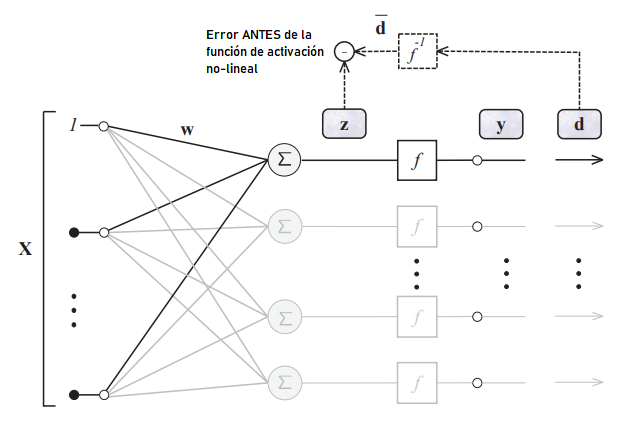
\includegraphics[scale=1]{Figuras/arquitectura_fedheonn.png}
        \caption{Arquitectura de la red neuronal de una sola capa \cite{paper_OLSVD}}
        \label{fig:fedheonn_arq}
    \end{subfigure}
    \vfill
    \vspace{0.5em}
    \begin{subfigure}{.9\linewidth}
        \centering
        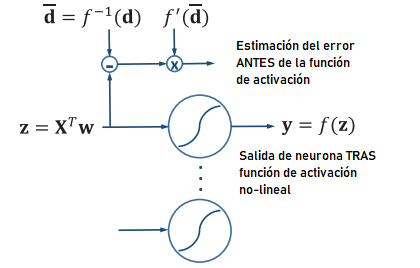
\includegraphics[scale=1]{Figuras/mse_antes.png}
        \caption{Estimación del error en la salida antes de la función de activación no-lineal \cite{paper_LANN}}
    \label{fig:fedheonn_mse}
    \end{subfigure}
\end{figure}

\noindent El error en la salida después de la función de activación se describe como:
\begin{equation}\label{eqn:error_mse}
    \mathcal{E} = \boldsymbol{d} - \boldsymbol{y} = \boldsymbol{d} - f(\boldsymbol{z}) = \boldsymbol{d} - f(\boldsymbol{X^T w}) \quad \footnotemark \quad \quad \mathcal{E} \in \mathbb{R}^{n \times 1}
\end{equation}

\noindent De modo que el error cuadrático medio MSE queda definido por:
\begin{equation}\label{eqn:mse_despues}
    \text{MSE} = \sum_{i=1}^n \mathcal{E}_i^2 = \|\mathcal{E}\|^2
\end{equation}


\footnotetext{Función de activación aplica componente a componente. $\bsym{v} \in \mathbb{R}^n \rightarrow f(\bsym{v}) = \left( f(\bsym{v}_1), f(\bsym{v}_2), \ldots, f(\bsym{v}_n) \right)^T$}

\noindent Podemos plantear ahora el error de salida \textbf{antes} de pasar por la función de activación como:
\begin{equation}\label{eqn:err_mse}
    \bar{\mathcal{E}} = \bar{\boldsymbol{d}} - \boldsymbol{z} = f\inv(\boldsymbol{d}) - \boldsymbol{X^T w} \quad \quad \bar{\mathcal{E}} \in \mathbb{R}^{n \times 1}
\end{equation}

\noindent Donde $f\inv:\;\mathbb{R}\rightarrow\mathbb{R}$ es la inversa de la función de activación. De \eqref{eqn:err_mse} también obtenemos la siguiente relación:
\begin{equation}
   \boldsymbol{z} = \bar{\boldsymbol{d}} - \bar{\mathcal{E}}
\end{equation}

\noindent Lo que nos permite introducir la siguiente aproximación de primer orden en serie de Taylor para cada componente del vector de salida $\boldsymbol{y}$:
\begin{equation}
    \boldsymbol{y} = f(\boldsymbol{z}) = f(\boldsymbol{\bar{d}-\bar{\mathcal{E}}}) \approx \underbrace{f(\boldsymbol{\bar{d}}) - f'(\boldsymbol{\bar{d}}) \circ \boldsymbol{\bar{\mathcal{E}}}}_\text{aprox. Taylor} = f(\boldsymbol{\bar{d}}) - f'(\boldsymbol{\bar{d}}) \circ (\bar{\boldsymbol{d}} - \boldsymbol{z})
\end{equation}

\noindent Con $f':\;\mathbb{R}\rightarrow\mathbb{R}$ la derivada de la función de activación y $ A \circ B$ el producto de \textit{Hadamard} o producto componente a componente.

\vspace{0.5em}

Esta última ecuación nos permite, finalmente, obtener una expresión del error en la salida en función de las salidas reales y las predichas antes de pasar por las funciones de activación no lineales (lo que denominamos $\boldsymbol{z}$) del siguiente modo, sustituyendo el resultado anterior en la ecuación \eqref{eqn:error_mse}:
\begin{align}
    \mathcal{E} = \boldsymbol{d} - \boldsymbol{y}  &= \boldsymbol{d} - f(\bar{\boldsymbol{d}}) + f'(\bar{\boldsymbol{d}})\circ(\bar{\boldsymbol{d}} - \bsym{z}) \nonumber \\
    &= \boldsymbol{d} - \bigl(f(f\inv(\boldsymbol{d}))\bigr) + f'(\bar{\boldsymbol{d}})\circ(\bar{\boldsymbol{d}} - \bsym{z}) \nonumber \\
    &= \boldsymbol{d} - \boldsymbol{d} + f'(\bar{\boldsymbol{d}})\circ(\bar{\boldsymbol{d}} - \bsym{z}) \nonumber \\
    &= f'(\bar{\boldsymbol{d}})\circ(\bar{\boldsymbol{d}} - \bsym{z}) = f'(\bar{\boldsymbol{d}})\circ(\bar{\boldsymbol{d}} - \boldsymbol{X^T w}) 
\end{align}

Definiendo ahora una matriz diagonal $\bsym{F}$ formada por la derivada de la función de activación \textit{f} sobre cada componente del vector $\bar{\boldsymbol{d}}$, es decir, $\boldsymbol{F} = diag\bigl(f'(\bar{\boldsymbol{d}_1}), f'(\bar{\boldsymbol{d}_2}), \ldots, f'(\bar{\boldsymbol{d}_n})\bigr)$, podemos reescribir la ecuación anterior y el MSE visto en \eqref{eqn:mse_despues} como:
\[
    \mathcal{E} = \boldsymbol{F}\,(\bar{\boldsymbol{d}} - \boldsymbol{X^T w})
\]
\begin{equation}\label{eqn:mse_final}
    \text{MSE} = \|\mathcal{E}\|^2 = \|\boldsymbol{F}\,(\bar{\boldsymbol{d}} - \boldsymbol{X^T w})\|^2 = \bigl( \boldsymbol{F} \, (\bar{\boldsymbol{d}} - \boldsymbol{X^T w})\bigr)^T  \bigl(\boldsymbol{F} \, (\bar{\boldsymbol{d}} - \boldsymbol{X^T w})\bigr)
\end{equation}

Con la ecuación \eqref{eqn:mse_final} podemos introducir ahora la \textbf{función objetivo} de este modelo, $\boldsymbol{J}(\boldsymbol{w})$, a la que se le añade un termino de regularización para evitar el sobreajuste o \textit{overfitting} basado en la normal L2 o \textit{rigde}, $\boldsymbol{R} = \frac{1}{2}\boldsymbol{w}^T\boldsymbol{w}$, de modo que queda:
\begin{equation}
    \boldsymbol{J}(\boldsymbol{w}) = \frac{1}{2} \biggl[\bigl( \boldsymbol{F} \, (\bar{\boldsymbol{d}} - \boldsymbol{X^T w})\bigr)^T  \bigl(\boldsymbol{F} \, (\bar{\boldsymbol{d}} - \boldsymbol{X^T w})\bigr) + \lambda\boldsymbol{w}^T\boldsymbol{w}\biggr]
\end{equation}

La función objetivo de la ecuación anterior tiene la ventaja de que, aún usando funciones de activación no lineales (\textit{f}), es \textbf{convexa} y presenta un mínimo global que puede ser obtenido directamente mediante solución cerrada para un $\boldsymbol{X}$ y $\boldsymbol{d}$ dados.

Este óptimo global se puede alcanzar fácilmente tras igualar a cero la derivada parcial de $\boldsymbol{J}$ respecto a los pesos. La derivación de dicha expresión resulta de aplicar la propiedad de linealidad, trasposición de producto y suma de matrices y la regla del producto. A continuación detallamos los pasos esenciales:
\[
    \boldsymbol{J}(\boldsymbol{w}) = \frac{1}{2} \biggl[
    \bigl(\boldsymbol{\bar{d}^T F^T} - \boldsymbol{w^TXF} \bigr) \bigl(\boldsymbol{F\bar{d}} -\boldsymbol{FX^Tw} \bigr) + \lambda \boldsymbol{w^Tw}
    \biggr]
\]
\begin{align*}
    \frac{\partial\boldsymbol{J(w)}}{\partial\boldsymbol{w}} &= \frac{1}{2} \biggl[ -\boldsymbol{XF}(\boldsymbol{F}\boldsymbol{\bar{d}} - \boldsymbol{FX^Tw}) + (\boldsymbol{\bar{d}^T F^T} - \boldsymbol{w^T XF})(-\boldsymbol{FX^T})+ 2\lambda\boldsymbol{w}\biggl] &= 0 \\
    &= \frac{1}{2} \biggl[ -\boldsymbol{XFF\bar{d}} + \boldsymbol{XFFX^Tw} -
       \underbrace{\boldsymbol{\bar{d}^T F^T FX^T}}_{XFF\bar{d}} + \underbrace{\boldsymbol{w^T XFFX^T}}_{XFFX^Tw} + 2\lambda\boldsymbol{w}\biggl] &= 0 \\
    &= \frac{1}{2} \biggl[ -2\boldsymbol{XFF\bar{d}} + 2\boldsymbol{XFFX^Tw} + 2\lambda\boldsymbol{w}\biggl] &= 0 \\
    &= -\boldsymbol{XFF\bar{d}} + \boldsymbol{XFFX^Tw} + \lambda\boldsymbol{w} &= 0 \\
    &= -\boldsymbol{XFF\bar{d}} + (\boldsymbol{XFFX^T} + \lambda\boldsymbol{I})\,\boldsymbol{w} &=0
\end{align*}

\noindent Que permite la construcción del sistema de ecuaciones lineales equivalente, $A \boldsymbol{w} = b$, cuya solución resulta en los \textbf{pesos óptimos} del modelo, que minimizan el MSE visto anteriormente:
\begin{equation} \label{eqn:sistema-ecuaciones-FL}
    (\boldsymbol{XFFX^T} + \lambda\boldsymbol{I})\,\boldsymbol{w} = \boldsymbol{XFF\bar{d}}
\end{equation}

El tamaño del sistema de ecuaciones \eqref{eqn:sistema-ecuaciones-FL} depende de $m$, el número de atributos del conjunto de datos, con una complejidad computacional superior de $O(m^3)$ para el cálculo de la inversa de la matriz $(\boldsymbol{XFFX^T} + \lambda\boldsymbol{I})$. Esto implica gran eficiencia sobre conjuntos de datos con un alto número de muestras y pocos atributos pero pobre rendimiento sobre conjuntos con muchas características, como es el caso de los \textit{microarrays}. Para obtener los pesos óptimos del modo más eficiente posible{ }--{ }independientemente del aspecto del conjunto de datos{ }--{ }se introdujo, en trabajos posteriores, una transformación del sistema lineal \eqref{eqn:sistema-ecuaciones-FL} a través de la factorización de la matriz $\bsym{XF}$, realizada mediante descomposición en valores singulares \textbf{SVD}:
\begin{equation*}
    \boldsymbol{XF} = \boldsymbol{USV^T}\quad \quad 
    \quad \boldsymbol{U} \in \mathbb{R}^{m \times m}\quad \boldsymbol{V} \in \mathbb{R}^{n \times n}\quad \boldsymbol{S} \in \mathbb{R}^{m \times n}
\end{equation*}
\noindent Con $\bsym{U}$ y $\bsym{V}$ matrices ortogonales y $\bsym{S}$ una matriz diagonal, de modo que resulta en un nuevo sistema de ecuaciones lineal:
\begin{equation}
    (\boldsymbol{USV^TFX^T} + \lambda\boldsymbol{I})\, \boldsymbol{w} = \boldsymbol{XFF\bar{d}}
\end{equation}
Cuya solución:
\begin{equation}\label{eqn:solucion_svd_fedheonn}
    \boldsymbol{w} = \boldsymbol{U}(\boldsymbol{SS^T} + \lambda \boldsymbol{I})\inv\boldsymbol{U^TXFF\bar{d}}
\end{equation}

Presenta ahora la ventaja de que, como $\bsym{S}$ es una matriz diagonal con $r \le min(m,n)$ elementos no nulos, las dimensiones efectivas de $\bsym{U}$ y $\bsym{S}$ son $\mathbb{R}^{m \times r}$ y $\mathbb{R}^{r \times r}$, respectivamente, lo que permite usar métodos SVD simplificados (sin calcular si quiera $\bsym{V}$), cuya \textbf{complejidad computacional} se reduce a $O(mnr)$. Esta descomposición es la operación más costosa, ya que la inversa de la matriz $(\boldsymbol{SS^T} + \lambda \boldsymbol{I})$, al ser diagonal para cualquier $\lambda \neq 0$, es trivial, al ser la inversa de las componentes diagonales, con complejidad $O(r)$.

\subsubsection{Aprendizaje federado y cifrado}

La solución anterior está formulada para el caso de un escenario centralizado, teniendo íntegramente a disposición la matriz de entrada del conjunto de datos $\bsym{X}$. Para adaptarlo al escenario federado, particularmente al conocido como \textit{Aprendizaje Federado Horizontal}, donde podemos suponer la matriz de entrada del \textit{dataset} como particionada en \textit{P} submatrices, de modo que $\boldsymbol{X} = [\boldsymbol{X_1|X_2|\ldots|X_P}]$, con cada cliente albergando una de estas submatrices, es necesario adaptar el algoritmo del siguiente modo:

\begin{itemize}[itemsep=2pt]
    \item Respecto a la matriz $\bsym{XF}$, factorizada mediante la descomposición en valores singulares SVD, se ha probado, como se estudia en el artículo publicado por M.A. Iwen et al \cite{svd_inc}, que dicha descomposición se puede obtener de un modo \textbf{incremental} y \textbf{distribuido}: 
    \begin{align}\label{eqn:svd_incremental}
        \text{SVD}(\bsym{XF})  
        &= \text{SVD}\bigl([\bsym{X}_1\bsym{F}_1 \mid \bsym{X}_2\bsym{F}_2 \mid \ldots \mid \bsym{X}_P\bsym{F}_P]\bigr) \nonumber \\
        &= \text{SVD}\bigl([\bsym{U}_1\bsym{S}_1 \mid \bsym{U}_2\bsym{S}_2 \mid \ldots \mid \bsym{U}_P\bsym{S}_P]\bigr)
    \end{align}
    Es decir, dada una matriz dividida en \textit{P} particiones, su descomposición SVD tiene los mismos valores singulares $\bsym{S}$ y valores singulares izquierdos $\bsym{U}$ que la matriz resultante de concatenar la descomposición del producto $\boldsymbol{U}_p \boldsymbol{S}_p$ de las submatrices.

    \item El término $\boldsymbol{XFF\bar{d}}$, que tanto en este trabajo como en el original, por simplicidad, denominamos $\boldsymbol{m} \in \mathbb{R}^{m\times1}$, se calcula de manera distribuida mediante el sumatorio de un producto de matrices que solo contienen la información de las submatrices de cada cliente como factores, pudiendo, por tanto, computarse incrementalmente mediante la adición de la información local $\boldsymbol{m}_p$ provista por cada nodo:
    \begin{equation}\label{eqn:m_incremental}
        \boldsymbol{m} = \boldsymbol{XFF\bar{d}} = 
        \sum_{p=1}^{P}\boldsymbol{X}_p\boldsymbol{F}_p\boldsymbol{F}_p \boldsymbol{\bar{d}}_p = \sum_{p=1}^{P} m_p
    \end{equation}
\end{itemize}

De esta manera, podemos crear un entorno federado con arquitectura cliente-servidor, en el que \textit{P} participantes (nodos){ }--{ }partiendo con la misma estructura de datos (en cuanto refiere a número de características){ }--{ }entrene colaborativamente el modelo de ML. Para hacerlo, cada cliente, usando su partición local de la matriz de datos de entrada $\boldsymbol{X}_p$, tendría que:

\begin{enumerate}[noitemsep]
    \item Calcular las submatrices $\boldsymbol{U}_p\,,\;\boldsymbol{S}_p$ resultado de la descomposición SVD de $\boldsymbol{X}_p\boldsymbol{F}_p$.
    \item Calcular el vector $\boldsymbol{m}_p = \boldsymbol{X}_p\boldsymbol{F}_p\boldsymbol{F}_p \boldsymbol{\bar{d}}_p$.
\end{enumerate}

El coordinador/servidor, por su parte, recibiría las matrices y vectores $\boldsymbol{U}_p\,,\;\boldsymbol{S}_p$ y $\boldsymbol{m}_p$ de cada cliente y agregaría la información al modelo global usando las ecuaciones \eqref{eqn:svd_incremental} y \eqref{eqn:m_incremental}. Con la información agregada, ya podría calcular los \textbf{pesos óptimos} según lo visto en la ecuación \eqref{eqn:solucion_svd_fedheonn}.

\vspace{0.5em}

El único aspecto restante es el \textbf{cifrado}. Aunque en el escenario federado trazado más arriba no hay transmisión alguna de datos en bruto a través de los nodos del modelo (garantizando la \textit{privacidad por diseño}), se decide añadir una capa más de seguridad mediante el uso de cifrado homomórfico, optando por cifrar el vector $\boldsymbol{m}_p$ de cada cliente por un par de motivos:

\begin{itemize}[noitemsep]
    \item El vector $\boldsymbol{m}_p$ puede ser más vulnerable a posibles ataques que las matrices fruto de la descomposición; $\boldsymbol{U}_p\,,\;\boldsymbol{S}_p$; que, sin la $\boldsymbol{V}^T_p$ correspondiente, no valen para recuperar la factorización original.
    \item La sucesiva adición de vectores encriptados homomórficamente está completamente soportada e ilimitada.
\end{itemize}

Para representar vectores y matrices encriptados, así como las operaciones entre ellos, usaremos la siguiente notación, $[[\;\cdot\;]]$. El tipo de encriptación homomórfica usada es de tipo FHE, mediante el esquema propuesto por Cheon, Kim, Kim y Song (\textbf{CKKS}, siglas de los autores del estudio '\textit{Homomorphic Encryption for Arithmetic of Approximate Numbers}' \cite{paper_CKKS}), que permite la operación con números reales.

\subsubsection{Algoritmos coordinador y clientes}
A continuación presentamos los algoritmos para coordinador y cliente del modelo de partida \textbf{FedHEONN}:

\begin{algorithm}[H]
\caption{Pseudocódigo para cliente FedHEONN}
\label{alg:fedclient}
\begin{algorithmic}[1]
\STATE \textbf{Entrada} para un cliente \textit{p}: 
    \STATE $\quad \bsym{X}_p \in \mathbb{R}^{m \times n_p}$ \hfill \COMMENT{Matriz de datos locales con \textit{m} atributos y \textit{n} muestras}
    \STATE $\quad \bsym{d}_p\; \in \mathbb{R}^{n_p \times 1}$ \hfill \COMMENT{Vector correspondiente con las salidas reales}
    \STATE $\quad f$ \hfill \COMMENT{Función de activación no lineal}
\STATE \textbf{Salida}:
    \STATE $\quad [\![\bsym{m}_p]\!]$ \hfill \COMMENT{Vector local $\bsym{m}$ encriptado}
    \STATE $\quad \bsym{US}_p$ \hfill \COMMENT{Matriz $\bsym{US}$ local}
\REQUIRE \verb|FEDHEONN_CLIENT|$(\boldsymbol{X}_p,\, \boldsymbol{d}_p,\, f):$
    \STATE $\quad \boldsymbol{X}_p \gets [\text{ones}(1,\, n_p); \boldsymbol{X}_p]$ \hfill \COMMENT{Se añade \textit{bias}}
    \STATE $\quad \boldsymbol{\bar{d}}_p \gets f\inv(\boldsymbol{d}_p)$ \hfill \COMMENT{Inversa de la función de activación}
    \STATE $\quad \boldsymbol{f}_p \gets f'(\boldsymbol{\bar{d}}_p)$ \hfill \COMMENT{Derivada de la función de activación}
    \STATE $\quad \boldsymbol{F}_p \gets \text{diag}(\boldsymbol{f}_p)$ \hfill \COMMENT{Matriz diagonal}
    \STATE $\quad [\bsym{U}_p, \bsym{S}_p, \sim] \gets \text{SVD}(\bsym{X}_p\,\bsym{F}_p)$ \hfill \COMMENT{SVD 'reducido'}
    \STATE $\quad \bsym{US}_p \gets \bsym{U}_p\,\text{diag}(\bsym{S}_p)$ \hfill \COMMENT{Producto de matrices locales $\bsym{U}_p\bsym{S}_p$}
    \STATE $\quad \bsym{m}_p \gets \bsym{X}_p \, (\bsym{f}_p \circ \bsym{f}_p \circ \bsym{\bar{d}}_p)$ \hfill \COMMENT{Vector local $\bsym{m}_p$}
    \STATE $\quad [\![\bsym{m}_p]\!] \gets \text{ckks\_encryption}(\bsym{m}_p)$ \hfill \COMMENT{Encriptación CKKS del vector $\bsym{m}_p$}
    \RETURN $[\![\bsym{m}_p]\!],\;\bsym{US}_p$
\ENSURE
\end{algorithmic}
\end{algorithm}

\begin{algorithm}[ht]
\caption{Pseudocódigo para coordinador FedHEONN}
\label{alg:fedcoord}
\begin{algorithmic}[1]
\STATE \textbf{Entrada}: 
    \STATE $\quad \bsym{M}_{list}$ \hfill \COMMENT{Lista con los vectores $\bsym{m}$ encriptados de los distintos clientes}
    \STATE $\quad \bsym{US}_{list}$ \hfill \COMMENT{Lista con las matrices $\bsym{US}$ de los distintos clientes}
    \STATE $\quad \lambda$ \hfill \COMMENT{Hiperparámetro de regularización}
\STATE \textbf{Salida}:
    \STATE $\quad [\![\bsym{w}]\!]\; \in \mathbb{R}^{m \times 1}$ \hfill \COMMENT{Pesos óptimos encriptados}
\REQUIRE \verb|FEDHEONN_COORDINATOR|$(\bsym{M}_{list},\, \bsym{US}_{list},\,\lambda):$
    \IF{existen matrices almacenadas $[\![\bsym{m}]\!],\; \bsym{US}$:}
        \STATE $[\![\bsym{m}]\!] \gets [\![\bsym{m}]\!]$ \text{ existente} \hfill \COMMENT{Vector $\bsym{m}$ inicializado}
        \STATE $\bsym{US} \gets \bsym{US}$ \text{ existente} \hfill \COMMENT{Matriz $\bsym{US}$ inicializada}
    \ELSE
        \STATE $[\![\bsym{m}]\!] \gets \bsym{0}$ \hfill \COMMENT{Vector de ceros}
        \STATE $\bsym{US} \gets [\ ]$ \hfill \COMMENT{Matriz vacía}
    \ENDIF
    \FOR{$[\![\bsym{m}_p]\!], \bsym{US}_p$ in $(M_{list}, US_{list})$}
        \STATE $[\![\bsym{m}]\!] \gets [\![\bsym{m}]\!] + [\![\bsym{m}_p]\!]$ \hfill \COMMENT{Agregamos vectores $\bsym{m}_p$}
        \STATE $[\bsym{U}, \bsym{S}, \sim] \gets \text{SVD}\bigl([\bsym{US} \mid \bsym{U}_p\bsym{S}_p]\bigr)$ \hfill \COMMENT{SVD incremental}
        \STATE $\bsym{US} \gets \bsym{U} \, \text{diag}(\bsym{S})$ \hfill \COMMENT{Agregación de matriz $\bsym{US}$}
    \ENDFOR
    \STATE $[\![\bsym{w}]\!] \gets \bsym{U} \, (\bsym{SS^T} + \lambda I)\inv \, (\bsym{U^T} \, [\![\bsym{m}]\!])$ \hfill \COMMENT{Calculamos pesos óptimos}
    \STATE Guardamos $[\![\bsym{m}]\!],\, \bsym{US}$ \hfill \COMMENT{Para agregar nueva información en el futuro}
    \RETURN $[\![\bsym{w}]\!]$
\ENSURE
\end{algorithmic}
\end{algorithm}

Podemos observar como, mientras cada cliente se limita a computar la matriz resultado del producto $\bsym{U}_p\bsym{S}_p$ y el vector encriptado $[\![\bsym{m}_p]\!]$ a partir de sus datos locales; es el coordinador el que realiza la mayor parte del trabajo agregándolos para cada cliente y calculando la solución del sistema global, vista en la ecuación \ref{eqn:solucion_svd_fedheonn}, una vez finalizado.

\vspace{0.5em}

Sobre este último punto cabe una última observación; para el cálculo de los pesos óptimos (línea 19 en algoritmo \ref{alg:fedcoord}) se producen \textbf{dos} multiplicaciones matriciales consecutivas, justo el límite superior de operaciones encadenadas de este tipo que se pueden realizar bajo el esquema CKKS de encriptación homomórfica que se usa en este trabajo, como se analizó en el artículo de Shereen Mohamed Fawaz et al \cite{seal_study}. Como dicha operación se realiza una vez agregada la información de los clientes, no depende del número de estos. La adición de vectores encriptados, como se menciona al final del apartado anterior, está ilimitada en el número máximo de operaciones sucesivas que se pueden realizar sin degenerar el resultado final.

\subsection{Agregación parcial e incremental}
La primera de las mejoras realizada en este trabajo sobre los algoritmos del modelo base \textbf{FedHEONN} para el cliente (algoritmo \ref{alg:fedclient}) y el coordinador (algoritmo \ref{alg:fedcoord}) fue la implementación de la agregación parcial e incremental, aspecto que teóricamente encontramos dispuesto pero cuya realización no se había probado.

\vspace{0.5em}

Los cambios necesarios para dicho ajuste son mínimos: el algoritmo del cliente permanece invariable y, en el algoritmo del coordinador, desglosamos la agregación parcial{ }--{ }con la información proveniente de los clientes{ }--{ }del propio cálculo de los pesos óptimos del sistema del modelo global, como se aprecia en los algoritmos \ref{alg:fedcoord_parcial} y \ref{alg:fedcoord_pesos}; siendo el único cambio significativo la separación de la matriz global existente $\bsym{US}$ en las matrices $\bsym{U}$ y $\bsym{S}$, para poder acceder a ellas individualmente desde ambas funciones.

\vspace{0.5em}

Esto permite, por un lado, \textbf{separar la agregación de la información de la obtención de los pesos óptimos}, que se puede realizar ahora en cualquier interludio de la progresiva incorporación de los datos de los clientes que, por otro lado, \textbf{ya no se tienen por que enviar en conjunto}; obligando a la espera y recopilación de las matrices y vectores $\bsym{U}_p\bsym{S}_p$ y $\bsym{m}_p$ de todos ellos (cuello de botella generado por el más lento de los clientes), si no que se pueden ir enviando lotes o pequeños grupos de ellos (incluso individualmente), según la disponibilidad presente o según finalicen sus respectivos entrenamientos locales.

\vspace{0.5em}

\textbf{Experimentalmente}, tenemos la necesidad de corroborar que esta aproximación a la agregación incremental de la información contenida en las matrices locales $\bsym{U}_p$, $\bsym{S}_p$ y $\bsym{m}_p$ por lotes sea igualmente efectiva que la vista en la ecuación \eqref{eqn:svd_incremental}. Para ello, supongamos ahora que los \textit{P} nodos (respectivas particiones de $\bsym{X}$) se agrupan en \textit{K} grupos, de modo que $\bsym{X} = [\bsym{X}_1|\ldots|\bsym{X}_P] = [\bsym{X}^{1} \mid \ldots \mid \bsym{X}^{K}]$, donde cada grupo $\bsym{X}^k$ puede albergar un subconjunto disjunto de nodos (es decir, distintas submatrices $\bsym{X}_p$) del conjunto total, tal que $\bsym{X}^{k} = \cup\,\bsym{X}_i\quad\forall{i}\,\in\mathcal{I}_k$, donde $\mathcal{I}_k$ es el conjunto de índices de los nodos/particiones pertenecientes al grupo $k$. Evidentemente, siempre se cumple $K \le P$, igualándose sólo en el caso de que cada grupo contenga un único nodo, aunque normalmente se tendrá que $K \ll P$. Es necesario demostrar que:
\begin{align}
\label{eqn:svd_parcial1}
\text{SVD}(\bsym{XF}) &= \text{SVD}\bigl([\bsym{X}_1\bsym{F}_1 \mid \ldots \mid \bsym{X}_P\bsym{F}_P]\bigr) = \text{SVD}\bigl([\bsym{U}_1 \bsym{S}_1 \mid \ldots \mid \boldsymbol{U}_P \boldsymbol{S}_P]\bigr) \nonumber \\
&= \text{SVD}\bigl([\bsym{X}^{1}\bsym{F}^{1} \mid \ldots \mid \bsym{X}^{K}\bsym{F}^{K}]\bigr) = \text{SVD}\bigl([\bsym{U}^1 \bsym{S}^1 \mid \ldots \mid \boldsymbol{U}^K \boldsymbol{S}^K]\bigr)
\end{align}

\noindent Donde $\bsym{U}^k\bsym{S}^k$ son, a su vez, las matrices de vectores singulares izquierdos y valores singulares correspondientes al $\text{SVD}(\cup\,[\bsym{X}_{i}\bsym{F}_i])\quad\forall{i}\in\mathcal{I}_k$.

\begin{algorithm}[ht]
\caption{Pseudocódigo para la \textbf{agregación parcial} en coordinador FedHEONN}
\label{alg:fedcoord_parcial}
\begin{algorithmic}[1]
\REQUIRE \verb|FEDHEONN_COORDINATOR:AGREGACION_PARCIAL|$(\bsym{M}_{grupo},\, \bsym{US}_{grupo}):$
    \IF{existen matrices almacenadas $[\![\bsym{m}]\!],\; \bsym{U},\; \bsym{S}$:}
        \STATE $[\![\bsym{m}]\!] \gets [\![\bsym{m}]\!]$ \text{ existente} \hfill \COMMENT{Vector $\bsym{m}$ inicializado}
        \STATE $\bsym{U} \gets \bsym{U}$ \text{ existente} \hfill \COMMENT{Matriz $\bsym{U}$ inicializada}
        \STATE $\bsym{S} \gets \bsym{S}$ \text{ existente} \hfill \COMMENT{Matriz $\bsym{S}$ inicializada}
    \ELSE
        \STATE $[\![\bsym{m}]\!] \gets \bsym{0}$ \hfill \COMMENT{Vector de ceros}
        \STATE $\bsym{U} \gets [\ ]$ \hfill \COMMENT{Matriz vacía}
        \STATE $\bsym{S} \gets [\ ]$
    \ENDIF
    \FOR{$[\![\bsym{m}_p]\!],\,\bsym{US}_p$ in $(\bsym{M}_{grupo}, \bsym{US}_{grupo})$}
        \STATE $[\bsym{U}, \bsym{S}, \sim] \gets \text{SVD}\bigl([\bsym{US} \mid \bsym{US}_p]\bigr)$ \hfill \COMMENT{Agregación incremental de matriz $\bsym{US}_p$}
        \STATE $[\![\bsym{m}]\!] \gets [\![\bsym{m}]\!] + [\![\bsym{m}_p]\!]$ \hfill \COMMENT{Agregamos vectores $\bsym{m}_p$}
    \ENDFOR
    \STATE Guardamos $[\![\bsym{m}]\!],\, \bsym{U},\, \bsym{S}$ \hfill \COMMENT{Para agregar nueva información en el futuro}
\ENSURE
\end{algorithmic}
\end{algorithm}

\begin{algorithm}
\caption{Pseudocódigo para calcular \textbf{pesos óptimos} en coordinador FedHEONN}
\label{alg:fedcoord_pesos}
\begin{algorithmic}[1]
    \REQUIRE \verb|FEDHEONN_COORDINATOR:CALCULAR_PESOS|$(\lambda):$
    \IF{existen matrices almacenadas $[\![\bsym{m}]\!],\; \bsym{U},\; \bsym{S}$:}
        \STATE $[\![\bsym{w}]\!] \gets \bsym{U} \, (\bsym{SS^T} + \lambda I)\inv \, (\bsym{U^T} \, [\![\bsym{m}]\!])$ \hfill \COMMENT{Calculamos pesos óptimos}
        \RETURN $[\![\bsym{w}]\!]$ \hfill \COMMENT{Vector $\bsym{w}$ encriptado}
    \ELSE
        \STATE \textbf{raise} error  \hfill \COMMENT{Lanzamos error}
    \ENDIF
\ENSURE
\end{algorithmic}
\end{algorithm}

\subsection{Ensamblaje}
El siguiente desarrollo juega un papel central en la investigación realizada en este trabajo. Se trata de incorporar una técnica de ensamblaje al algoritmo para comprobar si podemos mejorar la \textbf{capacidad de representación} de esta sencilla red neuronal lineal (se puede imaginar como un \textit{perceptrón} de una sola capa), y darle así la versatilidad necesaria para que destaque en escenarios federados compuestos por nodos de escasa potencia computacional que equilibren eficiencia y eficacia.

\vspace{0.5em}

El ensamblaje o \textit{ensemble} son métodos que, en esencia, combinan múltiples modelos (denominados \textit{estimadores base}) para mejorar el rendimiento y exactitud de las predicciones. La idea principal es que, al combinar varios modelos, bien con algoritmos de aprendizaje distintos, bien con matrices de datos (\textit{datasets}) diferentes, se pueden reducir los errores que podrían darse al usar un único modelo.

Aunque existen múltiples técnicas de ensamblaje, las dos fundamentales y más conocidas son las de tipo \textbf{bagging} y \textbf{boosting}. Esta última construye una serie de modelos secuencialmente donde cada uno trata de corregir los fallos cometidos por los anteriores, poniendo énfasis en las predicciones erróneas realizadas; mientras que, con la primera, se crean simultáneamente versiones de un modelo utilizando subconjuntos diferentes de los datos de entrenamiento, promediando sus predicciones.

El \textbf{boosting} tiene un enfoque, durante su entrenamiento,  \textit{secuencial}, ya que depende de las predicciones del estimador anterior para poder preparar y equilibrar el conjunto de datos de entrenamiento del siguiente, forzando un mayor número de rondas de comunicación entre servidor y clientes en un escenario federado; mientras que el \textbf{bagging}, al contrario, posibilita la \textit{paralelización} de dicho entrenamiento, ya que los estimadores base son independientes unos de otros.

Como el modelo de partida presenta unas características muy singulares como la naturaleza no iterativa de su entrenamiento, debido a la solución cerrada de los pesos óptimos globales, nos pareció más apropiado implementar una técnica de tipo \textit{bagging} a FedHEONN, que una de tipo \textit{boosting}, aunque suelan presentar mejores rendimientos.

\subsubsection*{Random Patches: una generalización del Bagging} \label{sec:random_patches_sol}

La técnica específica que se ha implementado en este trabajo es la denominada \textbf{Random Patches}, presentada en el artículo publicado por Gilles Louppe et al. \cite{random_patches}, como la máxima generalización del \textit{bootstrap aggregating}. Básicamente se crea un \textit{ensemble} de estimadores base entrenados a partir de ciertos \textit{parches} de los datos de entrenamiento, generados a través de la extracción aleatoria de subconjuntos de muestras y atributos. En dicho estudio se analiza como esta técnica iguala e incluso mejora métricas obtenidas por otros métodos de este tipo, al tiempo que reduce las necesidades de memoria.

% FORMAL
\paragraph*{Descripción}\mbox{}\\
La técnica propuesta puede ser descrita formalmente del siguiente modo: sea $R(\rho_s,\,\rho_f,\,D)$ el conjunto de todos los \textit{parches} de tamaño $\rho_s N_s \times \rho_f N_f$ que se pueden extraer del conjunto de datos $D$, donde $N_s$ es el número de muestras y $N_f$ el número de atributos en $D$ y donde $\rho_s,\,\rho_f \in [0,1]$ son los hiperparámetros que controlan, respectivamente, el número de muestras y atributos en un \textit{parche}. Es decir, sea $R(\rho_s,\,\rho_f,\,D)$ la serie de todos los posibles subconjuntos de $\rho_s N_s$ muestras y $\rho_f N_f$ atributos de $D$, el método se aplica del siguiente modo:

\begin{enumerate}[noitemsep]
    \item \textbf{Extraer} un \textit{parche} $r \, \sim \, U(R(\rho_s,\,\rho_p,\,D))$ aleatoriamente según una distribución uniforme del conjunto.
    \item \textbf{Entrenar} un estimador base con el parche seleccionado $r$.
    \item \textbf{Repetir} los pasos 1-2 para un número $T$ de estimadores.
    \item \textbf{Promediar} las predicciones de los $T$ estimadores base, en caso de regresión, o usar un voto mayoritario para la clasificación.
\end{enumerate}

% MEMORIA, INCLUSO REDUCCION COMPUTO GLOBAL
\paragraph*{Memoria}\mbox{}\\
A parte de ser una estrategia competitiva a la hora de implementar un ensamblaje de tipo \textit{bagging}, otra ventaja de esta técnica es que, tanto en el contexto de grandes conjuntos de datos, como en el de dispositivos embebidos bajo fuertes restricciones de memoria; es decir, en toda situación en la que el tamaño del conjunto de datos es mucho mayor que la memoria disponible, usar parches aleatorios del tamaño apropiado, sacados de los datos de entrenamiento, para construir estimadores base puede resultar en un modelo final tan bueno, o más, que como si todos los datos se hubieran podido cargar y usar directamente.

\vspace{0.5em}

Formalmente supongamos que, cuantificando la memoria utilizada por una unidad de datos como $M$, nos encontramos en un contexto tal que estamos restringidos a un umbral superior determinado por $M_{max}$; de modo que $M_{max}$ se pueda entender como el número total de unidades de memoria que se pueden cargar y utilizar en un determinado modelo. \footnote{No tenemos en cuenta la memoria utilizada por el propio modelo durante el transcurso de las operaciones inherentes a su algoritmo de entrenamiento.}

\vspace{0.5em}

En este escenario, la cantidad de memoria requerida por un \textit{random-patch} sería $(\rho_s N_s)(\rho_f N_f)$ y, por tanto, restringir la memoria en $M_{max}$ es equivalente a limitar el tamaño relativo del \textit{parche} a: 
\[
    \rho_s \rho_f \le \frac{M_{max}}{N_s N_f}
\]

\vspace{0.5em}
% EXPERIMENTOS - PRIMERO sensitivity ACCURACY, LUEGO EFICIENCIA
\noindent Los \textbf{experimentos} realizados con esta técnica pretender comprobar:
\begin{itemize}[noitemsep]
    \item Que, efectivamente, con este método se pueden conseguir \textbf{mejores métricas y rendimientos} que bajo la versión original de FedHEONN.
    \item Analizar la \textbf{sensibilidad de distintos conjuntos} ${\bigl(\rho_s,\,\rho_f,\,Acc_{D}(\rho_s,\,\rho_f)\;\mid\;\forall \rho_s,\,\rho_f \bigr)}$ sobre varios \textit{datasets} $D$, siendo $Acc_{D}(\rho_s,\,\rho_f)$ la exactitud media del ensamblaje construido con parches aleatorios de tamaño relativo $\rho_s\,\rho_f$.
    \item Comparar la \textbf{eficiencia} entre los mejores resultados obtenidos bajo esta técnica y los del modelo original, así como métricas equivalentes a estas últimas pero con mayor eficiencia y menor consumo de memoria (a base de usar un \textit{ensemble} de pocos parches y pequeño tamaño relativo).
\end{itemize}

\subsubsection*{Implementación en FedHEONN}

A continuación se describe el método de \textit{ensemble} desarrollado en este proyecto empleando como modelo base el FedHEONN. En esencia, los cambios necesarios en los algoritmos de cliente y coordinador fueron los siguientes:

\vspace{0.5em}

\noindent \textbf{Cliente}
\begin{itemize}[noitemsep]
    \item Añadimos el conjunto de hiperparámetros $(\rho_s,\,\beta_s,\,\rho_f,\,\beta_f,\,T)$ para precisar el tamaño relativo de los \textit{parches} $[\rho_s,\,\rho_f]$, si estos se extraen \textbf{con o sin reemplazo}, con los \textit{flags} $[\beta_s,\,\beta_f]$, y el número de estimadores base $T$ involucrados en el ensamblaje.
    \item Se \textit{envuelve} la función descrita en el algoritmo \ref{alg:fedclient} por una encargada de extraer aleatoriamente los \textit{parches} del conjunto de datos local, pasarlos por la función anterior de entrenamiento (\textit{fit}) y acumular sus resultados en una lista, para posterior envío al coordinador.
    \item Por último, y del mismo modo, se \textit{superpone} a la función de predicción (\textit{predict}), que introducimos en el algoritmo \ref{alg:fedcoord_client_ensemble_predict}, otra encargada de obtener las predicciones para cada conjunto de pesos óptimos de cada estimador base $T$ y, con los resultados, realizar el promedio o voto mayoritario dependiendo de si estamos ante un problema de regresión o de clasificación.
\end{itemize}

\vspace{0.5em}

\noindent \textbf{Coordinador}
\begin{itemize}[noitemsep]
    \item El único hiperparámetro necesario en el coordinador es un \textit{flag}, denominado \verb|ensemble|, para indicar si estamos ante un caso de ensamblaje o no, ya que el número de estimadores base $T$ se puede deducir a través de la longitud de la lista de matrices $[\![\bsym{m}_p]\!],\,\bsym{US}_p$ entregada por cada cliente.
    \item Se aplica por separado la agregación parcial y cálculo de pesos óptimos en cada \textit{i-ésimo} $[\![\bsym{m}_p^i]\!],\,\bsym{US}_p^i \mid \forall \, i = 1\dots T$ de cada cliente $P$, obteniendo una lista final de pesos óptimos $[\bsym{w}_1, \bsym{w}_2, \dots, \bsym{w}_T]$.
\end{itemize}

En definitiva, se trata de generalizar las fases de entrenamiento,  agregación y cálculo de pesos para realizarlas $T$ veces con cada parche aleatorio $\bsym{r}$ extraído del \textit{dataset} $D_p$ local correspondiente a cada cliente.

\subsubsection*{Sincronización de características}

La única dificultad y sobrecoste que implica este desarrollo radica en la necesidad de coordinar, entre los distintos nodos o clientes, exactamente cuales son los $\lfloor \rho_f N_f \rfloor$ atributos aleatorios seleccionados para la extracción del parche $\bsym{r}$-i-ésimo de cada estimador base $T$, ya que no podemos realizar la correcta agregación entre clientes de las matrices $[\![\bsym{m}_p^i]\!],\,\bsym{US}_p^i$ si estas no son el resultado del entrenamiento local sobre un $\bsym{X}_p^i \, \in \, \mathbb{R}^{(\rho_s m) \times (\rho_f n_p)}$ de las mismas características.

\vspace{0.5em}

Para ello se delegó esta tarea al coordinador, que ofrece ahora una función auxiliar capaz de generar una lista de $T$ series con los índices de los atributos seleccionados aleatoriamente, basándose en la fracción y número de atributos ($\rho_f,\,N_f$) entregado como argumento y de si se permite reemplazo o no ($\beta_f$).

\vspace{0.5em}

Esta lista es luego \textbf{enviada a todos los clientes} implicados en el aprendizaje federado, suponiendo una ronda de comunicación previa al entrenamiento de la red.

% TODO AÑADIR ALGORITMOS!
\subsubsection*{Algoritmos}

A continuación presentamos los algoritmos modificados para el cliente FedHEONN en sus tareas de entrenamiento y predicción, respectivamente algoritmos \ref{alg:fedcoord_client_ensemble} y \ref{alg:fedcoord_client_ensemble_predict}; para terminar con los correspondientes a la agregación parcial y cálculo de pesos óptimos, algoritmos \ref{alg:fedcoord_ensemble_aggregate} y \ref{alg:fedcoord_ensemble_optim}, en el coordinador.

%FIT CLIENT ENSENBLE
\begin{algorithm}[H]
\caption{Pseudocódigo para entrenamiento de cliente FedHEONN con \textbf{ensamblaje}}
\label{alg:fedcoord_client_ensemble}
\begin{algorithmic}[1]

    \STATE \textbf{Entrada} para un cliente \textit{p}:
    \STATE $\quad \bsym{X}_p \in \mathbb{R}^{m \times n_p},\; \bsym{d}_p\; \in \mathbb{R}^{n_p \times 1},\;f$ \hfill \COMMENT{Matriz de datos, vector de salidas y f.act.}
    \STATE $\quad T \in \mathbb{N}$ \hfill \COMMENT{Número de estimadores base}
    \STATE $\quad \rho_s \in (0,1]$ \hfill \COMMENT{Proporción del tamaño de muestras del parche}
    \STATE $\quad \beta_s :=$ \textbf{true or false} \hfill \COMMENT{Muestreo con reemplazo para registros}
    \STATE $\quad \rho_f \in (0,1]$ \hfill \COMMENT{Proporción del tamaño de atributos del parche}
    \STATE $\quad \beta_f :=$ \textbf{true or false} \hfill \COMMENT{Muestreo con reemplazo para atributos}
    \STATE \textbf{Salida}:
    \STATE $\quad \{[\![\bsym{m}_p^i]\!]\}_{i=1}^{T},\;\{\bsym{US}_p^i\}_{i=1}^{T}$ \hfill \COMMENT{Lista de $T$ vectores $\bsym{m}_p$ y matrices $\bsym{US}_p$}
    \STATE
    
    \REQUIRE \verb|FEDHEONN_CLIENT:FIT|$(\bsym{X}_p,\,\bsym{d}_p,\,f,\,T,\,\rho_s,\,\beta_s,\,\rho_f,\,\beta_f):$

    \STATE $\{\mathcal{I}_f\}_{i=1}^{T} \gets \texttt{FEDHEONN\_COORD:random\_attributes}(T,\,\rho_f,\,\beta_f,\,m)$ \hfill \COMMENT{Lista con $T$ series de índices aleatorios de atributos, generados y compartidos por el coordinador}
    
    \FOR{$i\;\text{in}\;T$}
        \STATE $\mathcal{I}_f \gets \{\mathcal{I}_f\}_i$ \hfill \COMMENT{Serie \textit{i-ésima} de índices de atributos aleatorios}
        
        \STATE $\mathcal{I}_s \gets \texttt{random\_choice}(\texttt{array=}n_p,\,\texttt{size=}\rho_s \times n_p,\,\texttt{replace=}\beta_s)$ \hfill \COMMENT{Índices muestras}
        
        \STATE $\bsym{X}_{p}^{i}\, \gets \bsym{X}_{p}[\mathcal{I}_f,\,\mathcal{I}_s]$ \hfill \COMMENT{Indexamos \textit{parche} de matriz de datos local}
        
        \STATE $\bsym{d}_{p}^{i}\, \gets \bsym{d}_{p}[\mathcal{I}_f,\,\mathcal{I}_s]$ \hfill \COMMENT{Indexamos \textit{parche} del vector de salidas local}
        
        \STATE $\{[\![\bsym{m}_p^i]\!]\},\;\{\bsym{US}_p^i\} \,   \gets \texttt{FEDHEONN\_CLIENT}(\bsym{X}_{p}^{i},\, \bsym{d}_{p}^{i},\, f)$ \hfill \COMMENT{Algoritmo \ref{alg:fedclient}}
        
    \ENDFOR
    
    \RETURN $\{[\![\bsym{m}_p^i]\!]\}_{i=1}^{T},\;\{\bsym{US}_p^i\}_{i=1}^{T}$ \hfill \COMMENT{Devolvemos lista de vectores y matrices}
    \ENSURE
\end{algorithmic}
\end{algorithm}

%PREDICT CLIENT ENSEMBLE
\begin{algorithm}[H]
\caption{Pseudocódigo para predicción en cliente FedHEONN con \textbf{ensamblaje}}
\label{alg:fedcoord_client_ensemble_predict}
\begin{algorithmic}[1]

    \STATE \textbf{Entrada} para un cliente \textit{p}:
    \STATE $\quad \bsym{X}_{p}^{test} \in \mathbb{R}^{m \times n_p}$ \hfill \COMMENT{Matriz de datos local de test o predicción}
    \STATE $\quad [\![\bsym{w}]\!] \in \mathbb{R}^{m \times1}$ \hfill \COMMENT{Vector de pesos óptimos encriptado}
    \STATE $\quad f$ \hfill \COMMENT{Función de activación}
    \STATE $\quad T \in \mathbb{N}$ \hfill \COMMENT{Número de estimadores base}
    \STATE $\quad \{\mathcal{I}_f\}_{i=1}^{T}$ \hfill \COMMENT{Serie de índices aleat. de atributos usados durante el entrenamiento}
    \STATE \textbf{Salida}:
    \STATE $\quad \bsym{y} \in \mathbb{R}^{n_p \times 1}$ \hfill \COMMENT{Vector de predicciones sobre test}
    \STATE

    \REQUIRE \verb|FEDHEONN_CLIENT:PREDICT_ENSEMBLE|$(\bsym{X}_{p}^{test},\,[\![\bsym{w}]\!],\,f,\,T,\,\{\mathcal{I}_f\}_{i=1}^{T}):$
    \STATE $\bsym{w} \gets \text{ckks\_decryption}([\![\bsym{w}]\!])$ \hfill \COMMENT{Desencriptamos vector de pesos óptimos}
    
    \FOR{$i\;\text{in}\;T$}
        \STATE $\mathcal{I}_f \gets \{\mathcal{I}_f\}_i$ \hfill \COMMENT{Serie \textit{i-ésima} de índices de atributos aleatorios}
        
        \STATE $\bsym{X}_{p}\, \gets \bsym{X}_{p}^{test}[\mathcal{I}_f,\,:]$ \hfill \COMMENT{Indexamos características de la matriz de datos de predicción}
        \STATE $\{\bsym{y}_i\} \, \gets \, \texttt{FEDHEONN\_CLIENT:PREDICT}(\bsym{X}_{p},\, \bsym{w},\, f)$ \hfill \COMMENT{Pred. estimador base \textit{i-ésimo}}
    \ENDFOR

    \IF[\hfill Para un problema de clasificación]{$\texttt{CLASIFICADOR}$}
        \STATE $\bsym{y}^{test} \gets \arg\max [\bsym{y}_1 \mid \bsym{y}_2 \mid \cdots \mid \bsym{y}_T]$ \hfill \COMMENT{Voto mayoritario}
    \ELSIF[\hfill Para un problema de regresión]{$\texttt{REGRESOR}$}
        \STATE $\bsym{y}^{test} \gets \frac{1}{T} \sum_{i=1}^{T} \bsym{y}_i$ \hfill \COMMENT{Promedio}
    \ENDIF

    \RETURN $\bsym{y}^{test}$ \hfill \COMMENT{Vector de predicciones}
    \ENSURE
    
    \STATE
    
    \REQUIRE \verb|FEDHEONN_CLIENT:PREDICT|$(\bsym{X}_{p},\,\bsym{w},\,f):$
    \STATE $\bsym{y} \gets f(\bsym{X}_{p}^T\,\bsym{w})$ \hfill \COMMENT{\textit{f} aplica componente a componente}
    \RETURN $\bsym{y}$
    \ENSURE
    
\end{algorithmic}
\end{algorithm}

%AGG COORD ENSEMBLE
\begin{algorithm}[H]
\caption{Pseudocódigo de agregación parcial en coordinador FedHEONN con \textbf{ensamblaje}}
\label{alg:fedcoord_ensemble_aggregate}
\begin{algorithmic}[1]
    \STATE \textbf{Entrada}:
    \STATE $\quad \{\bsym{M}_{grupo}\}$ \hfill \COMMENT{Lista\footnotemark\, de listas con lotes de vectores encriptados $\{[\![\bsym{m}_p^i]\!]\}_{i=1}^{T}$}
    \STATE $\quad \{\bsym{US}_{grupo}\}$ \hfill \COMMENT{Lista de listas con lotes de matrices locales $\{[\![\bsym{US}_p^i]\!]\}_{i=1}^{T}$}
    \REQUIRE \verb|FEDHEONN_CLIENT:AGG_PARCIAL_ENSEMBLE|$( \{\bsym{M}_{grupo}\},\,\{\bsym{US}_{grupo}\}):$
    \STATE $T \gets \text{length}(\{\bsym{M}_{{grupo}_1}\})$ \hfill \COMMENT{Deducimos nº de estimadores base}
    \FOR{$i\;\text{in}\;T$}
        \STATE $\bsym{M}_{grupo} \gets \{\bsym{M}_{{grupo}_i}\}$ \hfill \COMMENT{Seleccionamos lote \textit{i-ésimo}}
        \STATE $\bsym{US}_{grupo} \gets \{\bsym{US}_{{grupo}_i}\}$
        \STATE $\texttt{FEDHEON\_COORDINATOR:AGREGACION\_PARCIAL}(\bsym{M}_{grupo},\,\bsym{US}_{grupo})$ \hfill \COMMENT{Algoritmo \ref{alg:fedcoord_parcial}}
    \ENDFOR
\end{algorithmic}
\end{algorithm}

\footnotetext{Tanto $\{\bsym{M}_{grupo}\}$ como $\{\bsym{US}_{grupo}\}$ representan una lista de clientes, derivados de un determinado grupo $k$, y aportando cada uno, a su vez, un lote de matrices $\{[\![\bsym{m}_p^i]\!]\}_{i=1}^{T},\;\{\bsym{US}_p^i\}_{i=1}^{T}$ de sus respectivos estimadores base $T$.}

%OPTIM COORD ENSEMBLE
\begin{algorithm}[H]
\caption{Pseudocódigo cálculo pesos óptimos en coord. FedHEONN con \textbf{ensamblaje}}
\label{alg:fedcoord_ensemble_optim}
\begin{algorithmic}[1]
    \STATE \textbf{Salida}:
    \STATE $\quad \{[\![\bsym{w}]\!]\}_{i=1}^{T}$ \hfill \COMMENT{Lista de vectores encriptados con los pesos óptimos}
    \REQUIRE \verb|FEDHEONN_CLIENT:CALCULAR_PESOS_ENSEMBLE|$():$
    \IF{existen matrices almacenadas $\{[\![\bsym{m}]\!]\},\; \{\bsym{U}\},\; \{\bsym{S}\}$:}
        \STATE $T \gets \text{length}(\{[\![\bsym{m}]\!]\})$ \hfill \COMMENT{Deducimos nº estimadores base}
        \FOR{$i\;\text{in}\;T$}
            \STATE $[\![\bsym{m}]\!] \gets \{[\![\bsym{m}]\!]_i\}$ \hfill \COMMENT{Obtenemos matrices y vectores \textit{i-ésimos} globales almacenados}
            \STATE $[\![\bsym{U}]\!] \gets \{[\![\bsym{U}]\!]_i\}$
            \STATE $[\![\bsym{S}]\!] \gets \{[\![\bsym{S}]\!]_i\}$
            \STATE $[\![\bsym{w}_i]\!]\,\gets\,\texttt{FEDHEON\_COORDINATOR:CALCULAR\_PESOS()}$ \hfill \COMMENT{Algoritmo \ref{alg:fedcoord_pesos}}
        \ENDFOR
        \RETURN $\{[\![\bsym{w}_1]\!],\,[\![\bsym{w}_2]\!],\,\cdots,\,[\![\bsym{w}_T]\!]\}$
    \ELSE
        \STATE \textbf{raise} error  \hfill \COMMENT{Lanzamos error}
    \ENDIF
\end{algorithmic}
\end{algorithm}


\subsection{Paralelismo}
La siguiente mejora realizada al modelo FedHEONN con ensamblaje fue la capacidad de paralelizar el entrenamiento, en el cliente, y la agregación parcial y calculo de pesos óptimos, en el coordinador.

\vspace{0.5em}

Debido al incremento en el tiempo global de computo del entorno federado para casos con un gran número de estimadores base $T$, decidimos implementar esta solución como un modo de reducirlo y volverlo más eficiente, aprovechando la independencia entre estimadores que ofrece la técnica de \textit{bagging} aplicada anteriormente (cada estimador base \textit{i}-ésimo del nodo \textit{p} puede entrenar/agregar/calcularse partiendo únicamente de su conjunto de datos $\bsym{X}_p^i$ local).

\vspace{0.5em}

La única precaución durante su implementación fue asegurarse de mantener el orden de partida de los datos devueltos por los distintos procesos paralelos iniciados (\textit{pool de procesos}), cuyos tiempos y orden de finalización son imprevisibles \textit{a priori}, de modo que no mezclemos el orden de los estimadores base de ningún cliente.

\vspace{0.5em}

Con esta mejora se espera aprovechar la capacidad de los dispositivos físicos con procesadores multi-núcleo (\textit{multi-core}), que, aunque hace años solo estaban presentes en equipos personales, cada vez más se encuentran en todo tipo de sistemas móviles y embebidos, como, por ejemplo, las \textit{Rasberry Pi} y \textit{Jetson Nano} descritas en la sección \ref{sec:sist_infor}.

\vspace{1em}

\noindent\textbf{Experimentalmente} pretendemos comprobar que, a través de la paralelización:
\begin{itemize}[noitemsep]
    \item Podemos \textbf{acelerar}, individualmente y en conjunto, los procesos de entrenamiento, agregación y calculo de pesos óptimos.
    \item Comprobar a partir de que número de estimadores base $T$, para cierto par de $[\rho_s,\, \rho_f]$ y \textit{dataset} $D$, \textbf{compensa} la paralelización (debido a la \textit{sobrecarga} producida por la creación y manejo del \textit{pool} de procesos).
    \item Obtener así una especie de \textit{regla general} a partir de la cual es aconsejable activar dicha paralelización.
\end{itemize}

\subsubsection*{Implementación en FedHEONN}
Los totalidad de los detalles técnicos del desarrollo de esta mejora escapan a la envergadura de esta sección, donde solo pretendemos repasar, a modo de memoria, los procedimientos utilizados, las trabas encontradas y las soluciones aplicadas para sortearlas.

\vspace{0.5em}

La paralelización se realizó a través de la librería estándar de Python \verb|multiprocessing|, que presenta una API de alto nivel para el inicio y manejo de procesos. La idea original consistía en crear un \textit{pool} de procesos, tantos como \textit{cores} físicos dispone el CPU, para que se fuesen encargando de entrenar, agregar y calcular los pesos óptimos de cada estimador base involucrado en el \textit{ensemble} del modelo FedHEONN.

\vspace{0.5em}

El principal problema que se nos presentó con esta aproximación fue que la librería de encriptación homomórfica con la que estuvimos trabajando, TenSEAL, \textbf{no soporta} que las clases y objetos que define fuesen \textit{serializados}\footnote{Se denomina \textbf{serialización} al proceso encargado de convertir un objeto o estructura, en un determinado lenguaje de programación, a un formato que permita su almacenamiento, transmisión y futura reconstrucción a su estado original. Es muy útil para guardar el \textit{estado} de un objeto o enviarlo a través de la red.} a través del módulo estándar que usa Python para este tipo de protocolos, \verb|pickle|.

\vspace{0.5em}

Como los distintos procesos creados por el módulo de \verb|multiprocessing| \textbf{no comparten} el mismo espacio de memoria, cuando intentamos paralelizar el método de un objeto, Python intenta \textit{serializar} esta instancia, además de sus argumentos, usando \textit{pickle}, para compartirlos con los otros procesos creados; originando el problema descrito anteriormente.

\vspace{0.5em}

La librería \textbf{TenSEAL} expone sus propios métodos de serialización y de-serialización (\textit{reconstrucción}) de objetos de tipo \textit{CKKS} (vectores encriptados de números reales) y del propio \textit{contexto} de TenSEAL (custodia las llaves pública y privada de dicho esquema), por lo que, para implementar la paralelización en cliente y coordinador, hubo que realizar estas operaciones de manera programática mediante dichos métodos; de igual modo que lo hubiera hecho Python automáticamente a través de \textit{pickle}. Esto conlleva serializar fuera los argumentos que fuesen vectores encriptados, además del contexto de TenSEAL asociado, y reconstruirlos una vez dentro de toda función susceptible de ser paralelizable.

\vspace{0.5em}

Esto implicó un breve estudio secundario, no demasiado exhaustivo pero concluyente, para determinar que tipo de operaciones eran más costosas y saber así cuales merecían la paralelización, debido al añadido que suponen las operaciones de serialización y reconstrucción de los vectores involucrados. 

La encriptación de vectores y su adición son operaciones sencillas, mientras que encontramos la reconstrucción y serialización, tanto de contexto como vector, como operaciones muy costosas, al igual que la multiplicación de vectores encriptados. Con ello en mente, los cambios introducidos se resumen en:

\vspace{0.5em}

\noindent \textbf{Cliente}
\begin{itemize}[topsep=5pt, itemsep=2pt]
    \item La encriptación de los distintos vectores $[\![\bsym{m}_p^i]\!]$, al final del \textbf{entrenamiento} del cliente, se realiza ajena a cualquier parte de la paralelización, ya que el pequeño coste de dicha operación no compensa la \textit{sobrecarga} añadida por la serialización y reconstrucción del contexto necesario para ello.
    \item De esta manera, la paralelización en el cliente se realiza para toda la función descrita en el algoritmo \ref{alg:fedclient}, exceptuando la línea 15.
\end{itemize}

\noindent \textbf{Coordinador}
\begin{itemize}[topsep=5pt, itemsep=2pt]
    \item De manera muy parecida, en la \textbf{agregación parcial} se paraleliza todo el proceso involucrado con las matrices globales $\bsym{US}^i$ y las distintas $\bsym{US}_p^i$ de cada cliente (SVD), dejando la suma del término global $[\![\bsym{m}^i]\!]$ con los diferentes $[\![\bsym{m}_p^i]\!]$ aparte, ya que la suma de vectores encriptados \textit{CKKS} es una operación sencilla, y no compensa su serialización. Equivale a paralelizar solo las líneas 12-14 del algoritmo \ref{alg:fedcoord_parcial}.
    \item Para el \textbf{cálculo de pesos óptimos}, sin embargo, siempre que el número de estimadores base $T$ sea mayor al número de \textit{cores} físicos disponibles $_{cores}^{CPU}$, paralelizamos toda la función, agrupándose los estimadores en lotes equitativos a repartir entre tantos procesos como \textit{cores}, minimizando así el \textit{sobrecoste} de tener que serializar y reconstruir el contexto en cada proceso iniciado, ya que las dos multiplicaciones de matrices con vector encriptado involucradas en el cálculo de cada $\bsym{w}_i$ (línea 2 en el algoritmo \ref{alg:fedcoord_pesos}) compensa el coste computacional.
\end{itemize}


\subsection{Prototipo desarrollado para el entorno federado} \label{sec:servidor_sol}
Por último, desarrollamos una aplicación prototipo servidor-cliente, para demostrar el uso del modelo bajo un escenario realista de entorno federado, ya que todos los trabajos previos hasta la fecha habían simulado,  bajo un mismo equipo o dispositivo, tanto el coordinador como los distintos nodos involucrados en sus pruebas.

\vspace{0.5em}

Nos decantamos por utilizar la librería \textbf{FastAPI} para el desarrollo rápido de una interfaz de programación (Application Programming Interface, API) de tipo \textit{REST} (Representational State Transfer)\footnote{Una API de tipo REST es una interfaz que permite la comunicación entre sistemas utilizando HTTP, a través de peticiones estándar donde los recursos se representan en formatos como JSON o XML. Es un estilo de arquitectura que favorece la escalabilidad y simplicidad entre cliente y servidor.}, que nos permita demostrar la agregación parcial de la información de los distintos clientes conectados a la red y la predicción de los pesos óptimos calculados con ella.

\vspace{0.5em}

Uno de los problemas que se manifestó durante este desarrollo fue el de la \textbf{serialización}, mencionado anteriormente, ya que es a través de este como podemos enviar y recibir los vectores encriptados de los distintos clientes al servidor; por lo que nuestra aplicación tiene que gestionar, a mayores de las funciones propias del modelo FedHEONN, otras para el manejo, serialización y reconstrucción de dichos vectores.

\vspace{0.5em}

Experimentalmente, el objetivo fundamental de esta aplicación es el de servir de \textbf{demostrador} de un caso realista de entrenamiento y validación en red de un modelo federado, sin mayor ambición que la de su propio funcionamiento.

\subsubsection*{Descripción de la API}
A continuación presentamos una breve lista y descripción de los métodos ofrecidos por la API del servidor y las funciones equivalentes añadidas al cliente para su consumo:

\begin{itemize}
    \item \textbf{Servicios de disponibilidad y estado}:
    \begin{figure}[H]
        \centering
        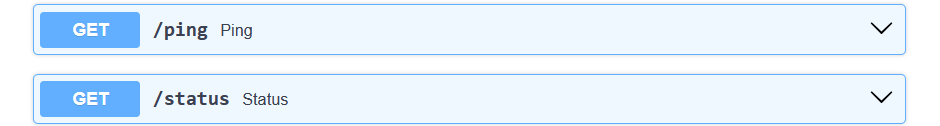
\includegraphics[width=\linewidth]{Figuras/api_estado.png}
        \caption{Endpoints para \textit{ping} y \textit{status} del servidor}    
    \end{figure}
    El primero es un servicio de \textit{ping}, para saber si el servidor está levantado y activo, mientras que el segundo, \textit{status}, devuelve un informe del estado actual del servidor, con, entre otros, el contexto TenSEAL seleccionado, el número de clientes agregados y procesados, etc., como veremos en la demostración del siguiente capítulo.
    \item \textbf{Servicios de selección y descarga de \textit{datasets}} $\bsym{D}_p$:
    \begin{figure}[H]
        \centering
        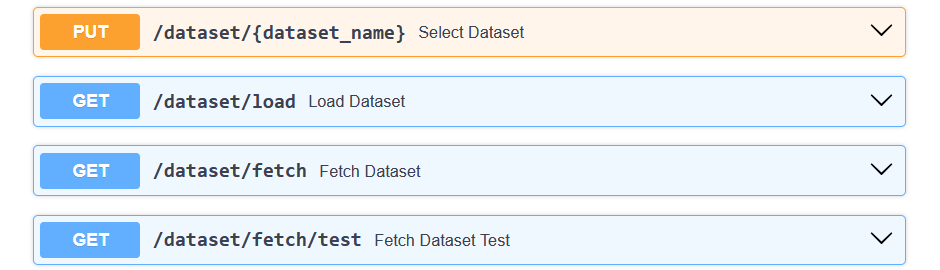
\includegraphics[width=\linewidth]{Figuras/api_dataset.png}
        \caption{Endpoints para la selección, carga y reparto de los datos de test y entrenamiento}    
    \end{figure}
    Estos servicios son los únicos que no tendrían cabida en un escenario realista, ya que lo que ofrecemos con ellos es la posibilidad de cargar distintos conjuntos de datos en el propio servidor (específicamente los vistos en la tabla \ref{tab:datasets}) y poder descargar fragmentos de distinto tamaño en cada cliente.
    
    Esto se consigue mediante sucesivas llamadas a un par de \textit{endpoints} (\verb|/dataset/fetch| y \verb|dataset/fetch/test|) hasta que se agoten los datos. Estos servicios se implementaron para poder realizar experimentos con los clientes bajo distintos tamaños de datos de entrenamiento en cada uno de ellos.
    
    \item \textbf{Servicios de gestión de contexto}:
    \begin{figure}[H]
        \centering
        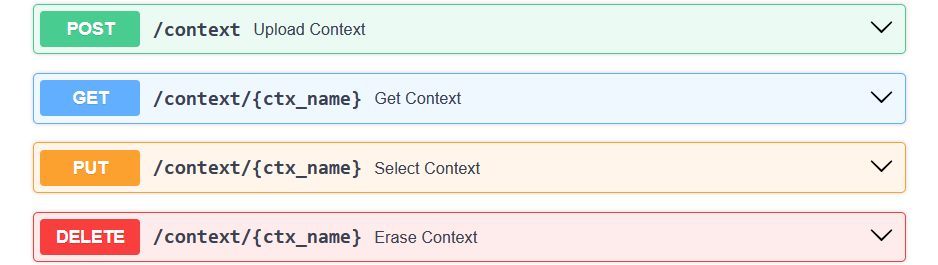
\includegraphics[width=\linewidth]{Figuras/api_contexto.png}
        \caption{Endpoints para la subida, selección, descarga y eliminación de contextos TenSEAL}    
    \end{figure}
    Los servicios anteriores permiten la gestión de los contextos de TenSEAL en el servidor, necesarios para la serialización y reconstrucción de la información (vectores \textit{CKKS}) enviada entre nodos y servidor.
    
    La idea aquí sería que un cliente o entidad de confianza (\textit{trusted party}) genere el contexto TenSEAL a utilizar (durante entrenamientos, agregación y calculo de pesos óptimo); y que lo subiese al servidor (públicamente, sin la clave privada asociada) mediante el \textit{endpoint} \verb|/context|. Una vez seleccionado este en el servidor, el resto de clientes involucrados podrían descargarlo a través de \verb|/context/{ctx_name}| y todos podrían realizar así las operaciones criptográficas necesarias.
    \item \textbf{Servicios de ajuste de hiperparámetros del coordinador}:
    \begin{figure}[ht]
        \centering
        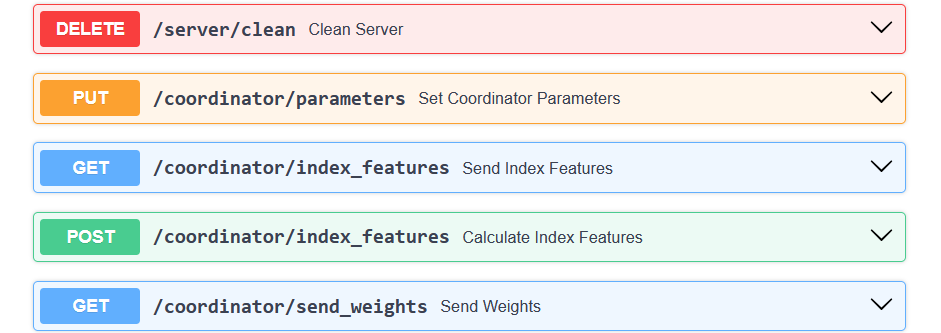
\includegraphics[width=\linewidth]{Figuras/api_coordinador.png}
        \caption{Endpoints para el ajuste de hiperparámetros, sincronización de características y envío de pesos óptimos del coordinador}
        \label{fig:coordinador_api_params}
    \end{figure}
    
    Los servicios relacionados con el coordinador FedHEONN permiten la actualización en el servidor, al cual está acoplado, de cualquiera de sus hiperparámetros (\textit{función de activación, regularización, ensamblaje, etc.}), como detallamos en la figura \ref{fig:hiperparm-server}.

    Además, se presenta también una fachada a las funciones de utilidad para la sincronización de características (vía \verb|/coordinator/index_features|), necesaria en el caso de realizar el entrenamiento con ensamblaje (como vimos en la sección \ref{sec:random_patches_sol}), que detallamos a continuación:
    \begin{enumerate}
        \item Un cliente o entidad de confianza pide al servidor que cree $T$ listas con $\rho_f N_f$ índices de atributos aleatorios, con/sin reemplazo.
        \item El resto de clientes descargan dichas listas para entrenar a sus estimadores base con $\bsym{X}_p^i$ semejantes.
    \end{enumerate}
    \begin{figure}[H]
        \begin{subfigure}{\textwidth}
            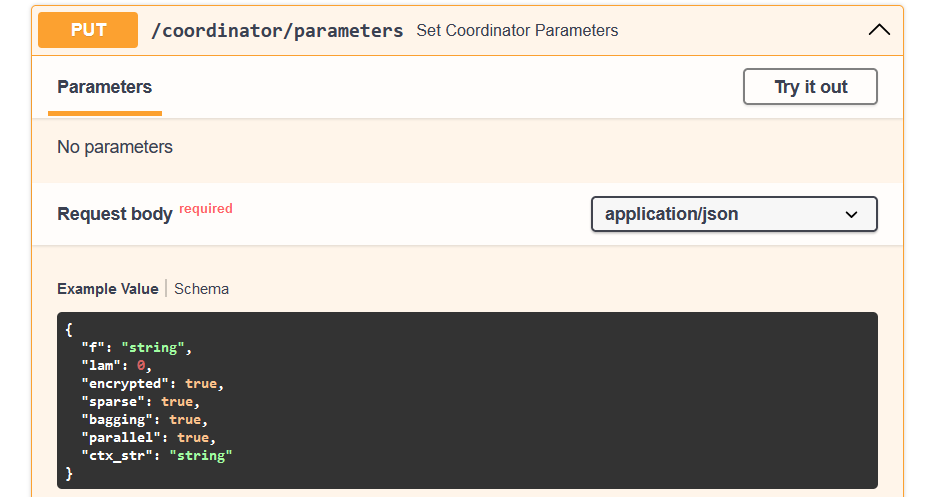
\includegraphics[height=.45\textwidth, width=\textwidth]{Figuras/api_coord_parameters.png}
            \caption{Detalle del servicio de actualización de hiperparámetros}
            \label{fig:hiperparm-server}
        \end{subfigure}
        \begin{subfigure}{\textwidth}
        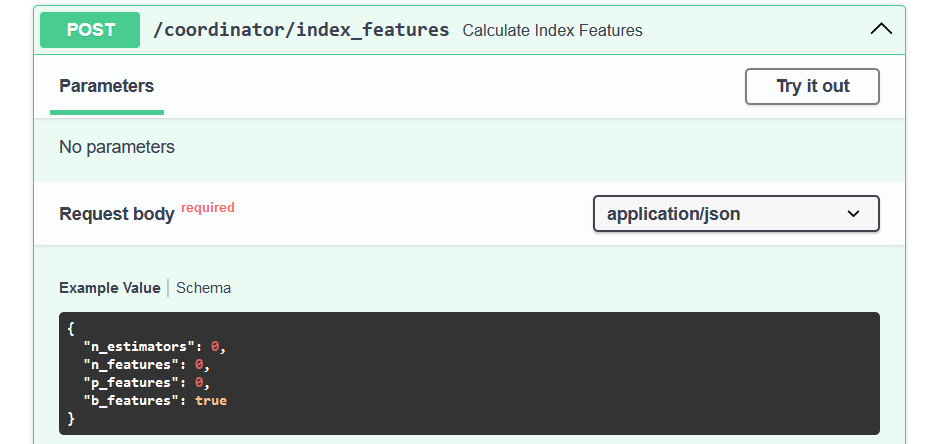
\includegraphics[height=.45\textwidth,width=\textwidth]{Figuras/api_coord_index.png}
            \caption{Detalle del servicio de sincronización de características}
            \label{fig:caracteristicas-server}
        \end{subfigure}
    \end{figure}
    \item \textbf{Servicios de agregación y cálculo de pesos óptimos}:
    \begin{figure}[H]
        \centering
        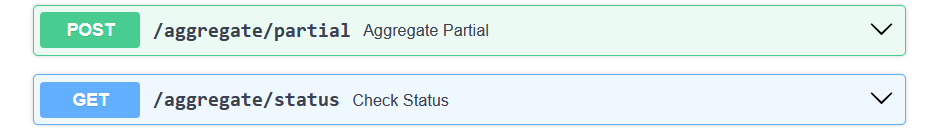
\includegraphics[width=\linewidth]{Figuras/api_agregacion.png}
        \caption{Endpoints para la \textit{agregación parcial} y comprobación de la cola de procesado}    
    \end{figure}
    Estos servicios son esenciales en la obtención del \textbf{modelo global} federado. Al primero, \verb|/aggregate/partial|, los diferentes clientes que constituyen la red federada deben enviar sus matrices $[\![\bsym{m}_p^i]\!],\,\bsym{US}_p^i$; quedando encoladas para su procesamiento por el coordinador, y obteniendo una serie de identificadores \textit{UUID} con los que pueden comprobar el estado de estas (pendientes, procesándose o ya procesadas).

    \vspace{0.5em}

    El \textit{endpoint} para la agregación parcial se ha diseñado de tal manera se encuentre \textbf{disponible} ante llamadas \textbf{concurrentes} y \textbf{consecutivas} (al igual que el resto de servicios del servidor), creando, en otro hilo (\textit{thread}), un bucle acoplado a una cola (\textit{queue}) que se encarga, de fondo, de ir agregando, incrementalmente, las matrices encoladas.

    \vspace{0.5em}
    
    Cuando esta cola se encuentra \textbf{vacía}, es decir, estamos ante un interludio donde ya se ha procesado toda la información recibida hasta el momento, se lanza automáticamente el \textbf{proceso de cálculo de pesos óptimos}. Estos pesos óptimos se pueden descargar, mediante el servicio \verb|/coordinator/send_weights|, visto en la figura \ref{fig:coordinador_api_params}, por los diferentes clientes, para realizar las predicciones oportunas con el modelo global.

    \vspace{0.5em}

    En el caso de que los clientes tengan acceso a la \textbf{clave privada} del contexto de TenSEAL utilizado durante el entrenamiento y agregación, podrán realizar la predicción desencriptando los pesos óptimos recibidos del servidor, $[\![\bsym{w}]\!]$, y luego aplicando $\bsym{y} = f(\bsym{z}) = f(\bsym{X^Tw})$. En caso contrario tendrían que recurrir a la entidad de confianza (\textit{trusted party}), depositaria de la clave privada, a la que podrían enviar, para mayor seguridad, el vector resultado del producto matricial de los pesos por la matriz de datos a predecir, $[\![\bsym{z}]\!]$, recibir dicho vector desencriptado $\bsym{z}$ y, finalmente, aplicarle la función de activación $\bsym{y} = f(\bsym{z})$.
\end{itemize}

Para los clientes se creó una clase con los respectivos métodos necesarios para consumir y comunicarse fácilmente con el servidor, conocida la dirección \textit{IP} y el puerto en el que este se encuentra escuchando, como se aprecia en la figura \ref{fig:api_cliente} (no mostramos todas las funciones).

\begin{figure}[H]
    \centering
    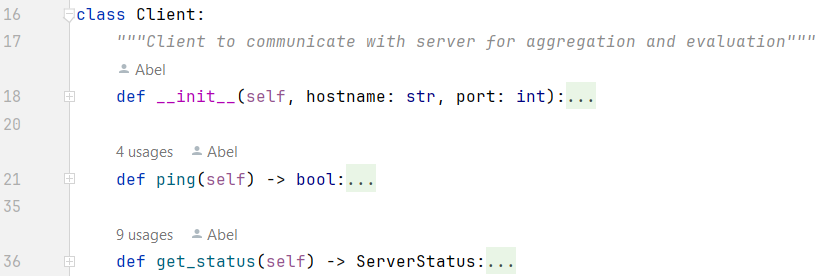
\includegraphics[width=.9\textwidth]{Figuras/cliente_api_estado.png}
    \caption{Clase cliente para consumo de API, con inicialización, \textit{ping} y \textit{status}}
    \label{fig:api_cliente}
\end{figure}

\newpage

\section{Resultados finales} \label{sec:resultados_final_anex}
En este capítulo presentamos los experimentos propuestos en los diferentes apartados de la sección anterior, manteniendo una estructura análoga y analizando los resultados obtenidos con ellos, dando fin así a la parte práctica de este trabajo y preparándonos para las conclusiones finales.

En cada sección detallaremos las pruebas realizadas y su implementación, así como los resultados esperados y obtenidos, finalizando con el nombre de los ficheros que albergan el código para su reproducción (bajo el directorio \verb|examples| en la estructura listada en la sección \ref{codigo_seccion}).

\subsection{Agregación parcial e incremental}
Las pruebas realizadas para verificar el correcto funcionamiento de la agregación parcial constan de tres fases:

\begin{enumerate}[topsep=2pt]
    \item Para un cierto \textit{dataset} $D$, realizamos lo que denominamos \verb|global_fit|, donde simplemente entrenamos y predecimos, usando la versión original del modelo vista en el algoritmo \ref{alg:fedcoord}, para un número dado de clientes $P$.
    \item Seguidamente, realizamos un \verb|incremental_fit|, agrupando los $P$ clientes en lotes de tamaño $N_g$, y efectuando con ellos la agregación parcial, cálculo de pesos óptimos (algoritmos \ref{alg:fedcoord_parcial} y \ref{alg:fedcoord_pesos}) y predicción sobre el mismo conjunto de \textit{test}.
    \item Por último, para un número distinto de clientes, $P'$, repetimos el proceso agrupándolos en lotes de tamaño aleatorio, que también entrenamos y testeamos incrementalmente del mismo modo.
\end{enumerate}

Con dichas pruebas se pretende comparar que las métricas obtenidas bajo dos escenarios distintos son equivalentes independientemente del procedimiento utilizado. La \textbf{agregación global} con $P$ clientes debería ser equivalente a la \textbf{incremental} de los mismos realizada en lotes de tamaño $N_g$, y esta última similar a la realizada con un número distinto de clientes $P'$ agrupados aleatoriamente.

Estas pruebas se realizaron sobre 3 conjuntos de datos distintos, definidos en la tabla \ref{tab:datasets}, y se encuentran en los ficheros \verb|classification_incremental*.py|, \texttt{regression\_increm\-ental*.py} y \verb|mnist.py| del directorio de \verb|examples|.

\vspace{0.5em}

A continuación presentamos algunos extractos de la salida de estos programas y un resumen de las pruebas de este apartado en la tabla \ref{tab:resultados_incremental}.

\begin{table}[H]
\resizebox{\textwidth}{!}{
\begin{tabular}{@{}llcccrr@{}}
\toprule
\textbf{Programa} &
  \textbf{Conjunto de datos} &
  \multicolumn{1}{l}{\textbf{P}} &
  \multicolumn{1}{l}{$\bsym{N}_g$} &
  \multicolumn{1}{l}{$\bsym{P'}$} &
  \multicolumn{1}{l}{\textbf{Métrica global}} &
  \multicolumn{1}{l}{\textbf{Métrica incremental}} \\ \midrule
classification\_incremental           & Dry Bean         & 1000 & 100 & -  & 90.30 \%		& 90.30 \% \\
classification\_incremental\_multiple & Dry Bean         & 1000 & 100 & 50 & 90.40 \%   	& 90.45 \% \\
regression\_incremental               & Carbon Nanotubes & 1000 & 100 & -  & 5.750e-5   	& 5.750E-05 \\
regression\_incremental\_multiple     & Carbon Nanotubes & 1000 & 100 & 50 & 5.750e-5   	& 5.749E-05 \\
mnist                                 & MNIST-test       & 10   & 2   & -  & 90.74 \%   	& 90.74 \% \\ \bottomrule
\end{tabular}
}
\caption{Resumen de los resultados experimentales de agregación parcial}
\label{tab:resultados_incremental}
\end{table}

\begin{figure}[H]
    \centering
    \begin{minipage}{0.49\textwidth}
        \centering
        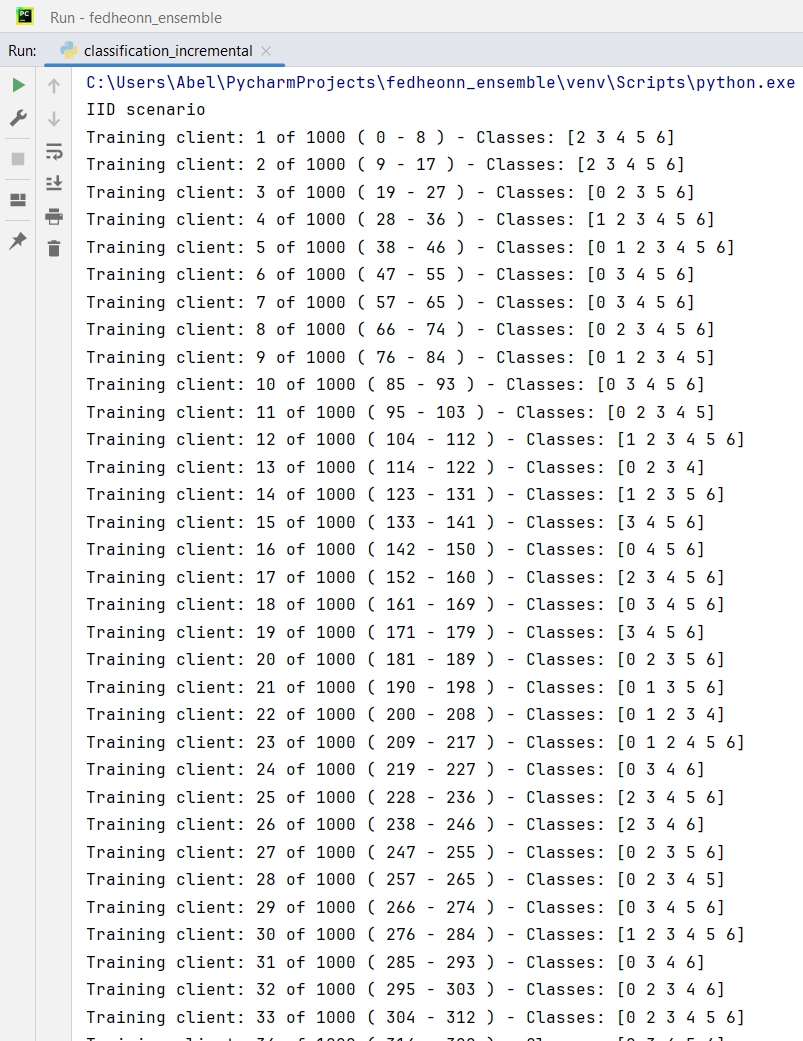
\includegraphics[width=\textwidth]{Figuras/agg_parcial_p0.png}
    \end{minipage}\hfill
    \begin{minipage}{0.49\textwidth}
        \centering
        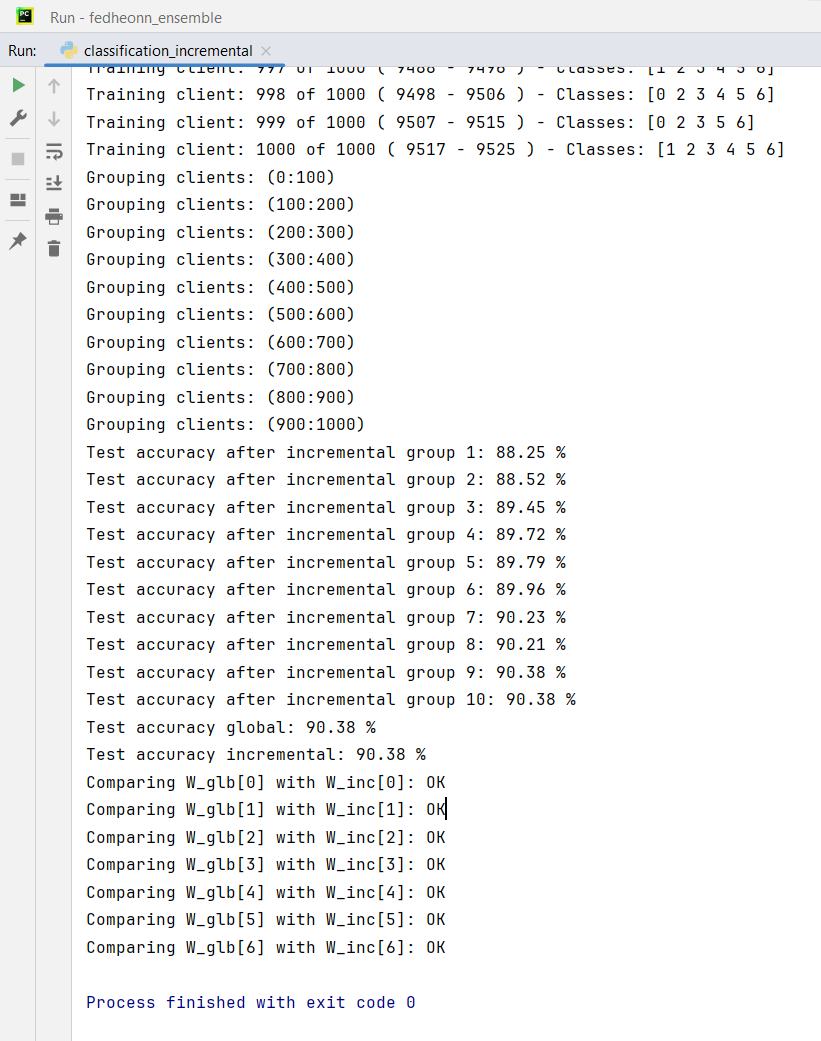
\includegraphics[width=\textwidth]{Figuras/agg_parcial_p1.png}
    \end{minipage}
    \caption{Salida de \texttt{classification\_incremental.py}}
    \label{fig:cla_inc}
\end{figure}

\begin{figure}[H]
    \centering
    \begin{minipage}{0.49\textwidth}
        \centering
        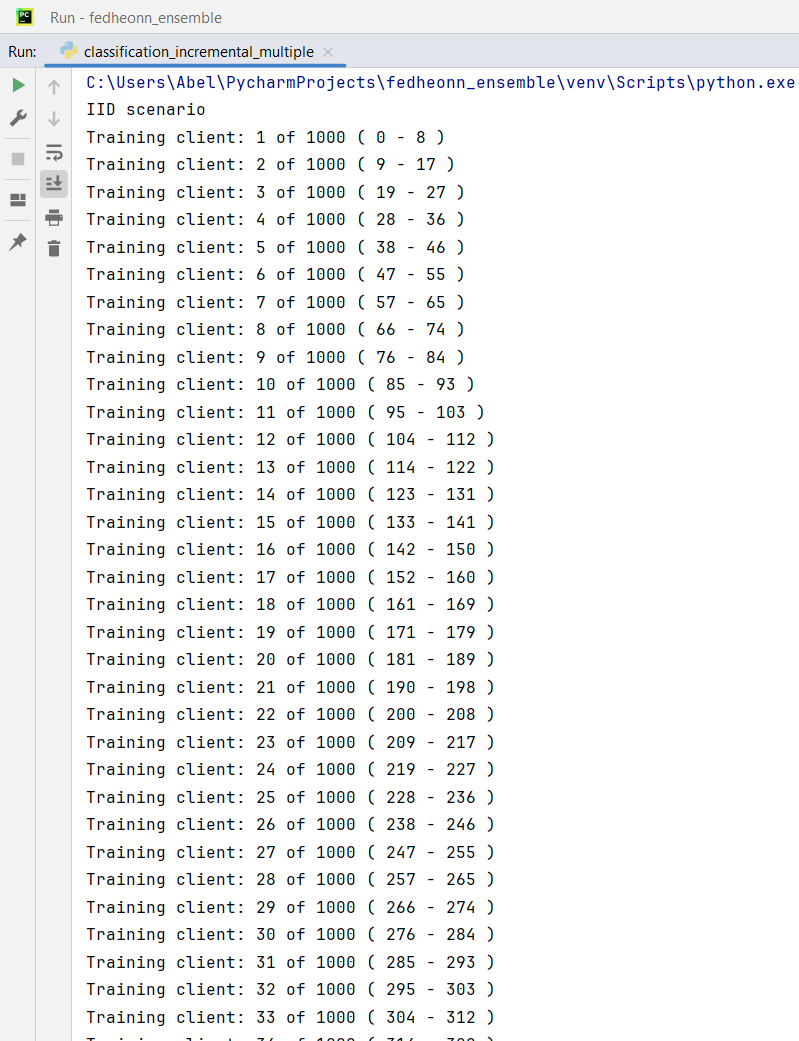
\includegraphics[height=1.3\textwidth,width=\textwidth]{Figuras/agg_parcial_p4.png}
    \end{minipage}\hfill
    \begin{minipage}{0.49\textwidth}
        \centering
        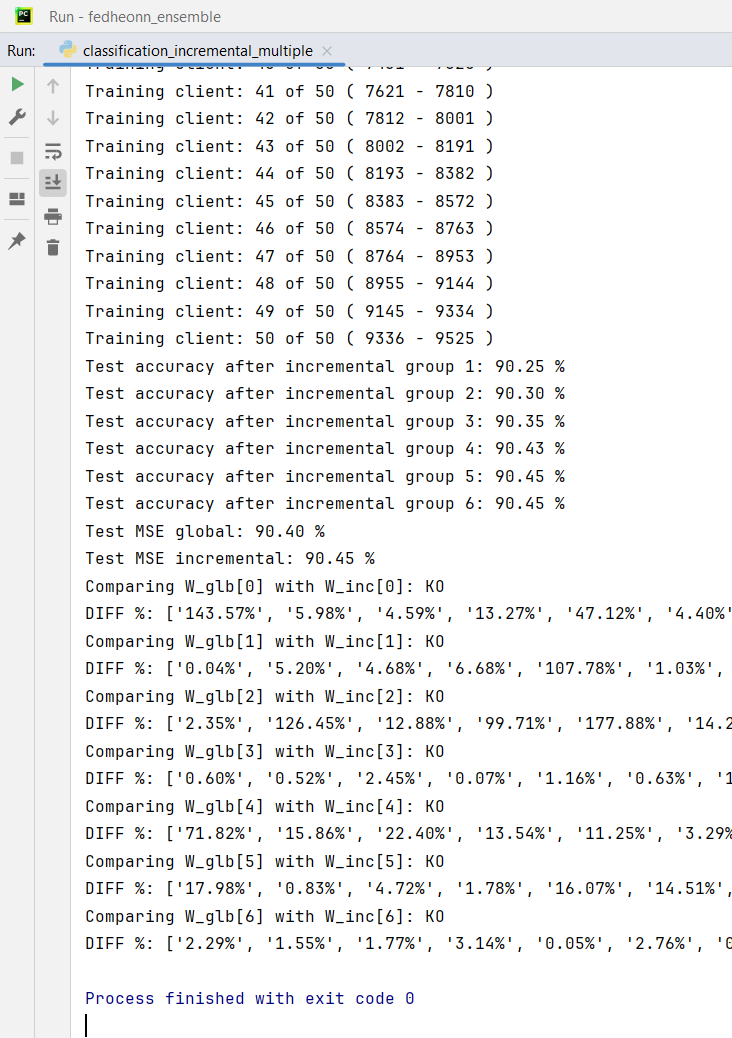
\includegraphics[height=1.3\textwidth,width=\textwidth]{Figuras/agg_parcial_p5.png}
    \end{minipage}
    \caption{Salida de \texttt{classification\_incremental\_multiple.py}}
    \label{fig:cla_mul}
\end{figure}

\begin{figure}[H]
    \centering
    \begin{minipage}{0.49\textwidth}
        \centering
        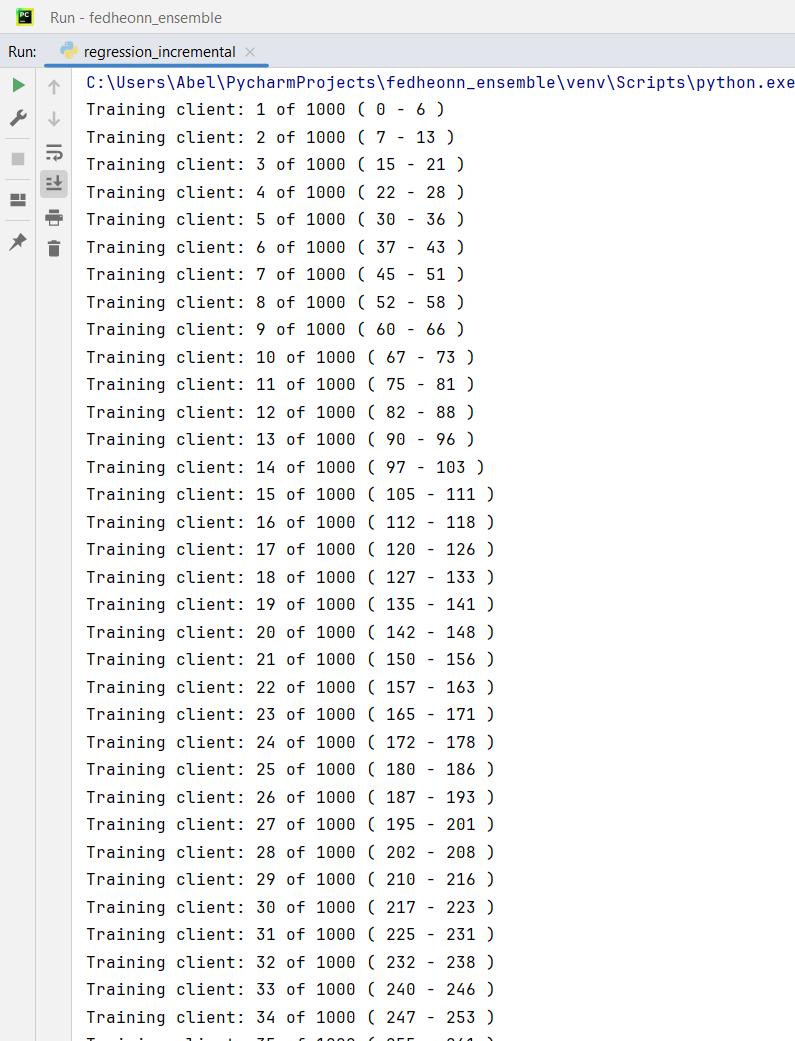
\includegraphics[height=1.3\textwidth,width=\textwidth]{Figuras/agg_parcial_p2.png}
    \end{minipage}\hfill
    \begin{minipage}{0.49\textwidth}
        \centering
        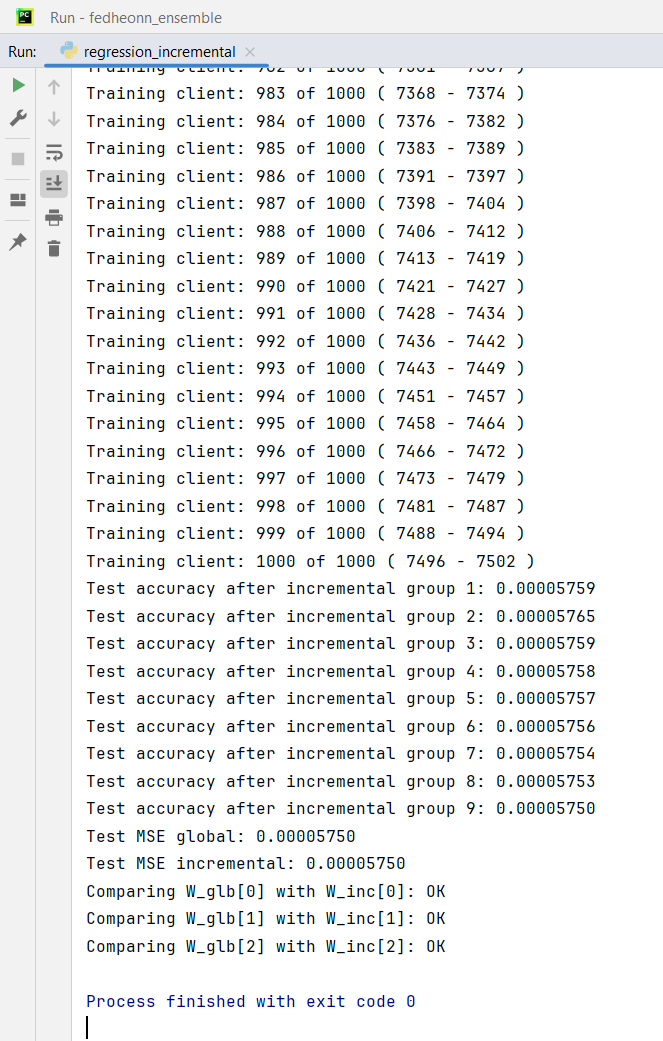
\includegraphics[height=1.3\textwidth,width=\textwidth]{Figuras/agg_parcial_p3.png}
    \end{minipage}
    \caption{Salida de \texttt{regression\_incremental.py}}
    \label{fig:reg_inc}
\end{figure}

\begin{figure}[H]
    \centering
    \begin{minipage}{0.49\textwidth}
        \centering
        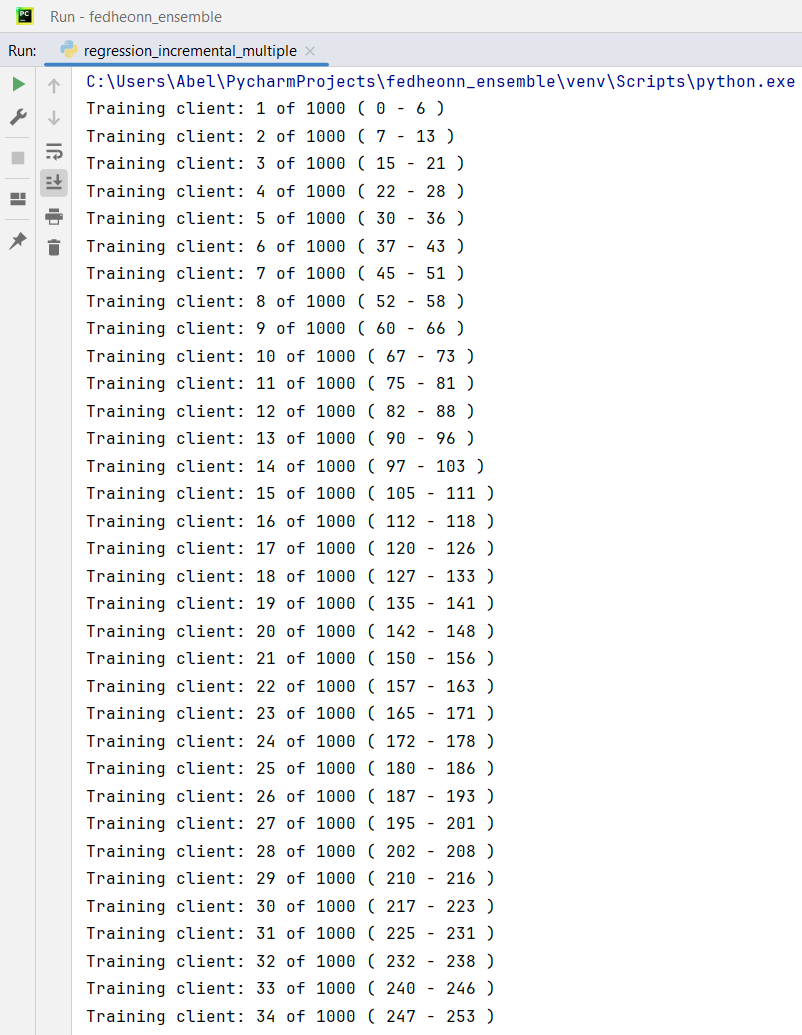
\includegraphics[height=1.3\textwidth,width=\textwidth]{Figuras/agg_parcial_p6.png}
    \end{minipage}\hfill
    \begin{minipage}{0.49\textwidth}
        \centering
        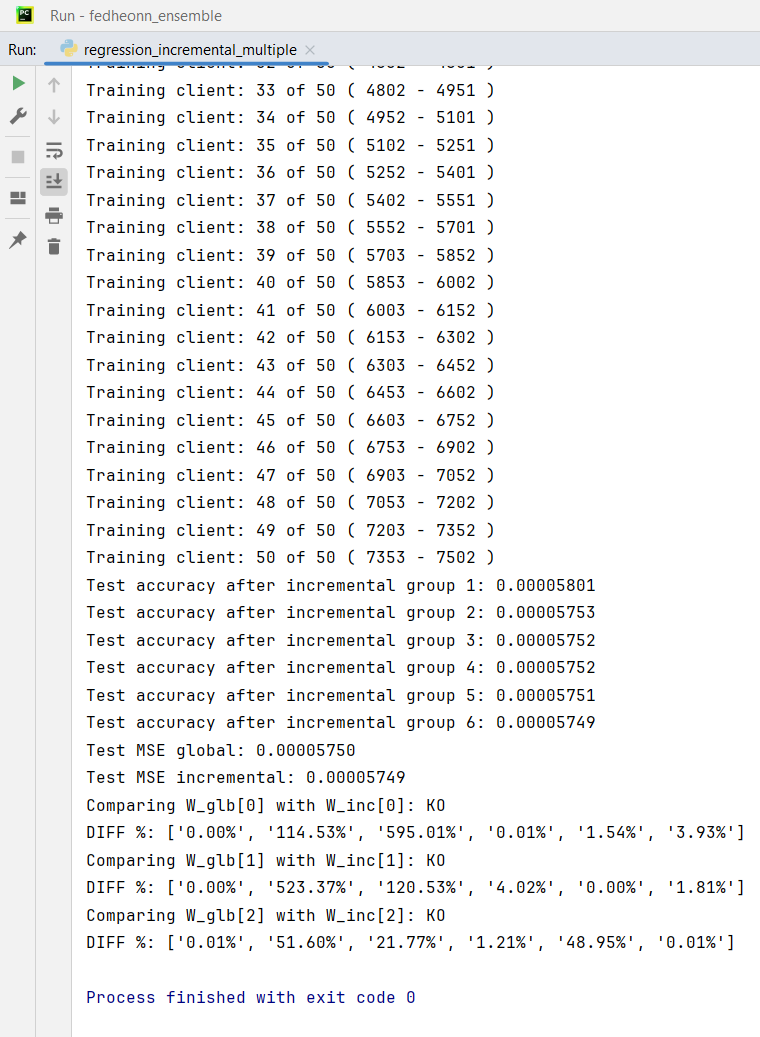
\includegraphics[height=1.3\textwidth,width=\textwidth]{Figuras/agg_parcial_p7.png}
    \end{minipage}
    \caption{Salida de \texttt{regression\_incremental\_multiple.py}}
    \label{fig:reg_mul}
\end{figure}

\begin{figure}[H]
    \centering
    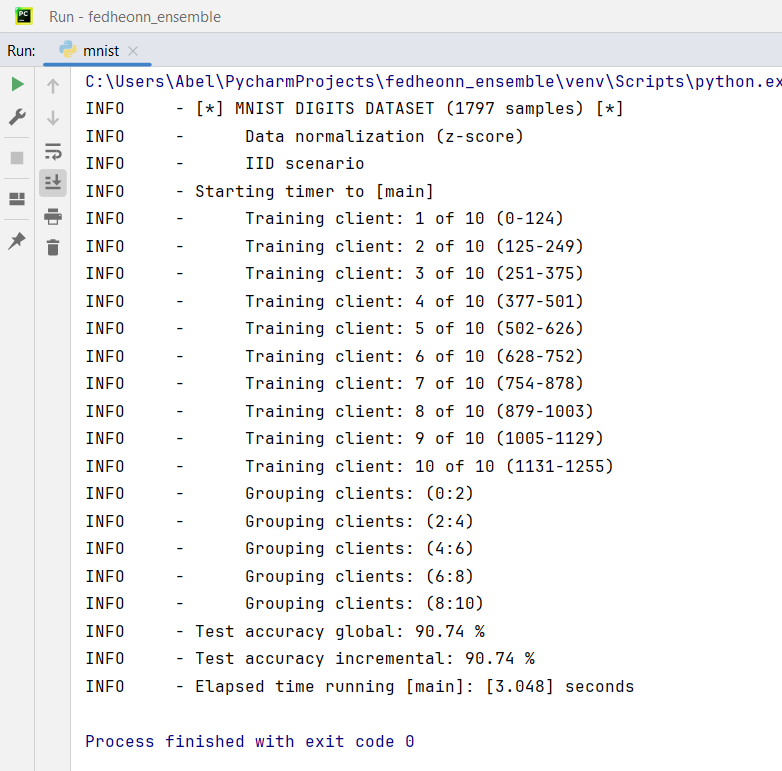
\includegraphics[scale=0.7]{Figuras/agg_parcial_p8.png}
    \caption{Salida de \texttt{mnist.py}}
    \label{fig:mnist_multiple}
\end{figure}

En la tabla \ref{tab:resultados_incremental} las métricas (columnas \textit{Métrica global} y \textit{Métrica incremental}) para las pruebas de clasificación corresponden a la exactitud, en \%, y el MSE para las de regresión.

\vspace{0.5em}

En los resultados correspondientes a \textit{classification\_incremental} y \textit{regression\_incremental}, figuras \ref{fig:cla_inc} y \ref{fig:reg_inc}, podemos observar como, para un mismo número de clientes $P$, la agregación global de todos ellos por separado, y la agregación parcial e incremental de estos en grupos de $N_g$ clientes, repercuten en métricas y pesos equivalentes. Este es también el caso de la última prueba, \verb|mnist|, correspondiente a la figura \ref{fig:mnist_multiple}.

\vspace{0.5em}

En cambio, en las pruebas con diferente número de clientes, correspondientes a \textit{classification\_incremental\_multiple} y \textit{regression\_incremental\_multiple}, figuras \ref{fig:cla_mul} y \ref{fig:reg_mul}, la agregación global de los primeros $P$ clientes y la incremental de los $P'$ segundos (en grupos aleatorios), no resultan en exactamente las mismas métricas, aún siendo bastante parecidas. Esto es debido a que, como el mismo \textit{dataset} $D$ está repartido entre un número distinto de clientes ($P \gg P'$), a su vez agrupados de distinto modo, el compendio de la información sobre el que entrenan unos y otros es distinto, repercutiendo en matrices $[\![\bsym{m}_p]\!],\,\bsym{US}_p$ semejantes pero no exactamente iguales.

\vspace{0.5em}

En definitiva, siempre que el número de clientes $P$ sea idéntico \textbf{se alcanzan matemáticamente los mismos resultados} tanto para en el algoritmo original de agregación y cálculo de pesos global como en los nuevos procesos independientes de agregación parcial en lotes y cálculo de pesos óptimos.


\subsection{Ensamblaje} \label{sec:result_ensamblaje}
La experimentación relativa a la implementación de la técnica de ensamblaje conocida como \textit{Random Patches} \cite{random_patches}, descrita en apartados anteriores, constaba de tres puntos: \textbf{primero}, probar que puede conseguir mejores rendimientos en algunos casos, \textbf{segundo}, analizar la sensibilidad de sus hiperparámetros sobre la exactitud para varios conjuntos distintos y, \textbf{tercero}, comparar la eficiencia de este modelo ampliado contra el original. Este último punto se analizará en la sección \ref{sec:res_eficiencia}, englobado con otros análisis energéticos, además de comparaciones con otro tipo de modelos.

\vspace{0.5em}

Comenzamos la experimentación con el \textbf{análisis de sensibilidad} sobre distintos conjuntos de datos, con respecto a la exactitud, realizando una búsqueda en cuadrícula tipo \textit{grid search}, efectuando una validación cruzada de tipo K-fold con 10 partes o \textit{splits} para cada serie de hiperparámetros $(T,\,\rho_s,\,\beta_s,\,\rho_f,\,\beta_f)$, resultando en una \textbf{exactidud media} y \textbf{desviación típica} generada por cada validación. Los conjuntos de datos usados, los rangos paramétricos seleccionados y el espacio de búsqueda total se detallan en la tabla \ref{fig:tabla_gridsearch}.

\begin{figure}[H]
    \centering
    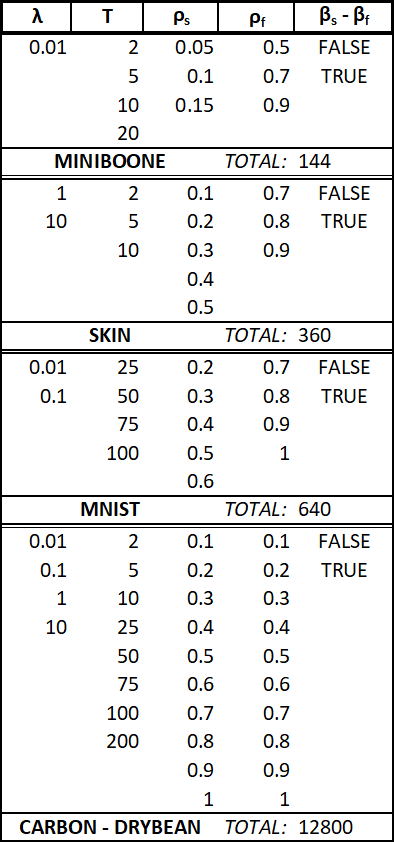
\includegraphics[scale=.8]{Figuras/tabla_gridsearch.png}
    \caption{Tabla con el rango paramétrico para los distintos \textit{grid-search} ejecutados}
    \label{fig:tabla_gridsearch}
\end{figure}

Los programas diseñados para realizar este \textit{cross-validation grid-search} se pueden encontrar bajo el nombre \verb|*_gridsearchcv_remote.py| en el directorio \verb|examples| y exportaron sus respectivos resultados a un fichero tipo Excel, de los que dejamos una copia bajo ese mismo directorio.

La longitud en la dimensión de los distintos espacios paramétricos es inversamente proporcional al tiempo de ejecución necesario para una iteración sobre los distintos conjuntos, de modo que; en aquellos con entrenamientos más pesados, como \textit{MiniBoone}, \textit{Skin} o \textit{MNIST}, se realizó un barrido previo más tosco para afinar el rango de valores adecuado de la búsqueda paramétrica.

En la sección \ref{sec:anexo_resultados} del anexo de resultados dejamos unas imágenes con la salida de estos programas, cuya ejecución tardó desde unas horas hasta un par de días (figuras \ref{fig:cmd_skin} a \ref{fig:cmd_carbon}), seguido de unas tablas con los resultados alcanzados para cada conjunto de datos, extraídos de los ficheros Excel exportados por los programas previos, y de las cuales se dirimen unas primeras conclusiones de este apartado (tablas \ref{tab:gscv_mnist} a \ref{tab:gscv_carbon_classic}):

\begin{itemize}[noitemsep, topsep=2pt]
    \item La \textbf{efectividad de esta técnica} en la exactitud es totalmente dependiente del conjunto de datos y estimador base utilizado (\textit{refiriéndonos al modelo sobre el que aplica}).
    \item Existen conjuntos de datos en los que su implementación \textbf{no repercute en ninguna mejora} apreciable y, por tanto, puede ser descartada.
\end{itemize}

\vspace{0.5em}

Las métricas óptimas obtenidas y los hiperparámetros correspondientes, tanto para la versión original del modelo, como para la versión que incorpora el ensamblaje, se presentan en la tabla \ref{tab:bagging_cv}.

%TODO TABLA
\begin{table}[h]
\centering
\resizebox{\textwidth}{!}{
\begin{tabular}{@{}lrcccccccc@{}}
\toprule

\textbf{Conjunto de datos}\tablefootnote{Las filas con conjuntos y resultados en negrita representan la versión con ensamblaje.} &
$\bsym{\lambda}$ (\textbf{reg.}) &
\textbf{f.act.} &
$\bsym{T}$ &
$\bsym{\rho_s}$ &
$\bsym{\beta_s}$ &
$\bsym{\rho_f}$ &
$\bsym{\beta_f}$ &
\multicolumn{2}{c}{\textbf{\begin{tabular}[c]{@{}c@{}}Exactitud o MSE\\ $(\bsym{\mu},\,\bsym{\sigma})$\end{tabular}}} \\ \midrule
  
MNIST-test 					& 0.01	& \textit{logs} 	& -	& -   	& - 			& -   & - & 88.15 \%  & 3.14 \% \\
\textbf{MNIST-test} 		& 0.01 	& \textit{logs} 	& 75	& 0.2 	& \checkmark 	& 0.8 & X & \textbf{95.94 \%} & \textbf{2.37} \% \\
Skin       					& 10   	& \textit{logs} 	& -	& -   	& - 			& -   & - & 80.52 \% & 0.31 \% \\
\textbf{Skin}       		& 10   	& \textit{logs} 	& 2	& 0.1 	& X 			& 0.7 & \checkmark & \textbf{84.21 \%} & \textbf{0.34 \%} \\
MiniBoone       			& 0.01	& \textit{logs} 	& -	& - 	& - 			& - & - & 85.34 \% & 0.30 \% \\
\textbf{MiniBoone}			& 0.01	& \textit{logs} 	& 2	& 0.05 	& X 			& 0.9 & X & \textbf{86.85 \%} & \textbf{0.33 \%} \\
Dry Bean       				& 0.01	& \textit{logs} 	& -	& - 	& - 			& - & - & 90.69 \% & 1.01 \% \\
\textbf{Dry Bean}			& 0.01	& \textit{logs} 	& 10	& 0.8 	& \checkmark 	& 1 & X & \textbf{91.01 \%} & \textbf{1.03 \%} \\
Carbon Nanotubes			& 0.01	& \textit{linear} 	& -	& - 	& - 			&	 - & - & 7.85E-05 & 8.70E-05 \\
\textbf{Carbon Nanotubes}	& 0.01	& \textit{linear} 	& 75	& 0.4 	& \checkmark 	& 1 & X & \textbf{7.83E-05} & \textbf{8.69E-05} \\ \bottomrule
\end{tabular}
}
\caption{Resultados del modelo con ensamblaje con los hiperparámetros óptimos obtenidos con validación cruzada}
\label{tab:bagging_cv}
\end{table}

Como se puede apreciar, las diferencias en algunos casos son significativas, destacando una \textbf{mejora} de casi un \textbf{8 \%} en la exactitud para el caso del conjunto de datos \textit{MNIST-test} y casi un \textbf{4 \%} para el conjunto \textit{Skin}, de las versiones con ensamblaje respecto a las originales, usando ambos los mismos hiperparámetros (a excepción de los propios del \textit{ensemble}). En el resto de conjuntos la mejora es más discreta, del 1 y 0.5 \% respectivamente para la exactidud en \textit{MiniBoone} y \textit{Dry Bean}, y una reducción de $0.02\times10^{-5}$, o un 0.25 \% relativo, para el MSE de \textit{Carbon Nanotubes}.

\vspace{0.5em}

Los hiperparámetros propios del ensamblaje tipo \textit{Random Patches} de la tabla \ref{tab:bagging_cv} usados han sido aquellos que ofrecieron mejores métricas para cada conjunto, luego de realizar la búsqueda paramétrica detallada al inicio, que, aún sin ser demasiado exhaustiva, da pie a observar que:

\begin{itemize}[noitemsep, topsep=2pt]
    \item Un alto número de estimadores base $T$ no tiene por que resultar en mejores métricas.
    \item Se abre un amplio espacio de búsqueda nuevo, para dar con el ajuste más eficaz y/o eficiente de este tipo de ensamblaje.
\end{itemize}

\subsection{Paralelismo}
De forma muy parecida, las pruebas de este apartado se centrarán en \textbf{demostrar} que la paralelización del proceso, tanto en cliente como coordinador, es capaz de reducir los tiempos globales de ejecución y explorar, brevemente, como afectan ciertos hiperparámetros del ensamblaje, como el número de estimadores base $T$ o el tamaño relativo del parche $\rho_s \times \rho_f$ a dicha reducción.

\vspace{0.5em}

No merece la pena realizar estudios mayores{ }--{ }en primera instancia{ }--{ }ya que el principal factor en tal ahorro tiene también mucho que ver con las dimensiones del conjunto de entrenamiento y el número de clientes involucrados.

\vspace{0.5em}

En esta sección nos centraremos específicamente en el dataset \textit{MNIST-test} para todos los ejemplos siguientes, con un número de clientes $P$ de 4 y agrupados en lotes $N_g$ de 2 clientes.

\vspace{0.5em}

Para evidenciar el primer punto ejecutamos el programa \verb|mnist_parallel.py|, localizado en la carpeta \verb|examples|, donde se corre el entrenamiento global e incremental del modelo bajo un ensamblaje de $T = 50$ estimadores base y tamaño relativo del parche $(\rho_s \times \rho_f) = 1$; \textbf{con y sin paralelización}.

\vspace{0.5em}

En las figuras \ref{fig:mnist_par_serie} y \ref{fig:mnist_par_par} del anexo de resultados mostramos la salida de estos programas y en la tabla \ref{tbl:tabla_tiempos_paralelo} recopilamos sus resultados. En esta, hemos desglosado y cronometrado los tiempos de ejecución de las distintas tareas involucradas en el proceso de entrenamiento conjunto del modelo de la siguiente forma:

\begin{itemize}[noitemsep, topsep=2pt]
    \item Para la lista de clientes, recordemos $P = 4$, medimos el tiempo de entrenamiento de cada conjunto de datos local (\texttt{fit}).
    \item Para el coordinador central, la agregación y cálculo de pesos óptimos se realiza de modo \textit{global}, como en la versión original, y de modo \textit{incremental}, en lotes de $N_g = 2$, realizando primero la agregación parcial y, por último, el cálculo de pesos óptimos, en procesos separados.
    \item También hemos incluido el tiempo requerido para serializar el contexto y vectores encriptados, previo a su procesamiento en paralelo, necesario para las tareas de agregación (\texttt{aggregate}) y cálculo de pesos óptimos (\texttt{calc\_weights}), representando el preprocesamiento de estos casos (\texttt{pre-proc}).
\end{itemize}

%TABLA TIEMPOS
\begin{table}[h!]
\centering

\large{\textbf{Desglose de tiempos de ejecución (s)}}
\small
\vspace{0.5cm}
\begin{tabular}{@{}rrrrrr@{}}
\multicolumn{6}{c}{\textbf{EN SERIE}} \\ \midrule
\multicolumn{2}{c}{\textbf{Clientes}} & \multicolumn{4}{c}{\textbf{Coordinador}} \\ \midrule
\multicolumn{2}{c}{\textbf{FIT}}                & \multicolumn{2}{c}{\textbf{GLOBAL}}          & \multicolumn{2}{c}{\textbf{INCREMENTAL}}       \\ \midrule

\verb|CLIENTE 1:| & 23.29 & \verb|PRE-PROC:| & 0.00  & \verb|PRE-PROC:| & 0.00   \\ 
\verb|CLIENTE 2:| & 24.65 & \verb|AGGREGATE:| & 715.18 & \verb|AGG_PARTIAL 1:| & 2.90  \\ 
\verb|CLIENTE 3:| & 24.76 & \multicolumn{2}{c}{\texttt{-}} & \verb|AGG_PARTIAL 2:| & 5.26  \\ 
\verb|CLIENTE 4:| & 24.89 & \multicolumn{2}{c}{\texttt{-}} & \verb|CALC_WEIGHTS:| & 728.04  \\ \bottomrule

$\Sigma:\;$ & 97.59 & $\Sigma:\;$ & 716.57 & $\Sigma:\;$ & 737.53 \\ \hline
\end{tabular}

\vspace{0.2cm}

\begin{tabular}{@{}rrrrrr@{}}
\multicolumn{6}{c}{\textbf{EN PARALELO}} \\ \midrule
\multicolumn{2}{c}{\textbf{Clientes}} & \multicolumn{4}{c}{\textbf{Coordinador}} \\ \midrule
\multicolumn{2}{c}{\textbf{FIT}}                & \multicolumn{2}{c}{\textbf{GLOBAL}}          & \multicolumn{2}{c}{\textbf{INCREMENTAL}}       \\ \midrule

\verb|CLIENTE 1:| & 14.92 & \verb|PRE-PROC:| & 30.10  & \verb|PRE-PROC:| & 9.66   \\ 
\verb|CLIENTE 2:| & 14.86 & \verb|AGGREGATE:| & 728.46 & \verb|AGG_PARTIAL 1:| & 7.51  \\ 
\verb|CLIENTE 3:| & 16.22 & \multicolumn{2}{c}{\texttt{-}} & \verb|AGG_PARTIAL 2:| & 7.10  \\ 
\verb|CLIENTE 4:| & 16.13 & \multicolumn{2}{c}{\texttt{-}} & \verb|CALC_WEIGHTS:| & 692.22  \\ \bottomrule

$\Sigma:\;$ & 62.13 & $\Sigma:\;$ & 730.14 & $\Sigma:\;$ & 707.58 \\ \hline
\end{tabular}
\normalsize
\caption{Tiempos de ejecución de los distintos procesos involucrados en el entrenamiento conjunto de FedHEONN}
\label{tbl:tabla_tiempos_paralelo}
\end{table}

Se puede observar una \textbf{reducción significativa} en los tiempos de \textbf{entrenamiento} que concierne a los \textbf{clientes} de la red, siendo hasta $1/3$ más rápido para todos los casos, pasando de un \textit{fit} global de los clientes de $98\;(s)$ a $62\;(s)$, por ejemplo.

Por la contra, la \textbf{paralelización en el coordinador no resulta tan efectiva}. Cuando se efectúa una \textit{agregación global} (algoritmo original del modelo) con este ensamblaje, el proceso tarda más incluso que sin la paralelización, debido, en mayor parte, al gran coste añadido que supone el preprocesado de datos (serialización y deserialización de contexto y vectores) y creación y manejo de procesos necesarios para ello. Por ejemplo, medio minuto, $30\; (s)$ de los $728\; (s)$ de dicha agregación se destinaron únicamente a serializar y preparar en lotes los datos necesarios para cada proceso del \textit{pool}.

El mismo problema se aprecia también en la nueva versión, denominada \textit{incremental}, donde separamos la agregación de los datos del cálculo de pesos óptimos; aquí, la \textbf{paralelización de la primera (\texttt{agg\_partial}) tarda más en ejecutarse} que su equivalente en serie (debido al \textit{sobrecoste} del manejo de los procesos), pero, por la contra, el \textbf{proceso de cálculo de pesos óptimos (\texttt{calculate\_weights}) si que se redujo, aproximadamente, en un 5 \%}, de $728\;(s)$ a $692\;(s)$.

\vspace{0.5em}

En las gráficas de la figura \ref{fig:par_experiments}, creadas con el programa \texttt{mnist\_parallel\_tests.py} del directorio de \verb|examples|, representamos los tiempos de ejecución de los distintos procesos del modelo vistos anteriormente; específicamente, el \textit{fit} de los clientes y la \textit{agregación parcial} y \textit{cálculo de pesos óptimos} del coordinador, según el número de estimadores base $T$ empleados, \textbf{en serie y en paralelo}.

\begin{figure}[ht]
    \centering
    \begin{subfigure}[b]{0.49\textwidth}
        \centering
        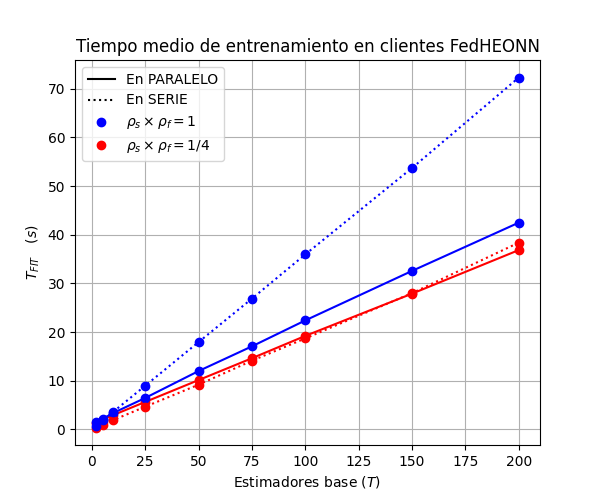
\includegraphics[width=\textwidth]{Figuras/tiempo_fit.png}
        \label{fig:par_fit1}
    \end{subfigure}
    \hfill
    \begin{subfigure}[b]{0.49\textwidth}
        \centering
        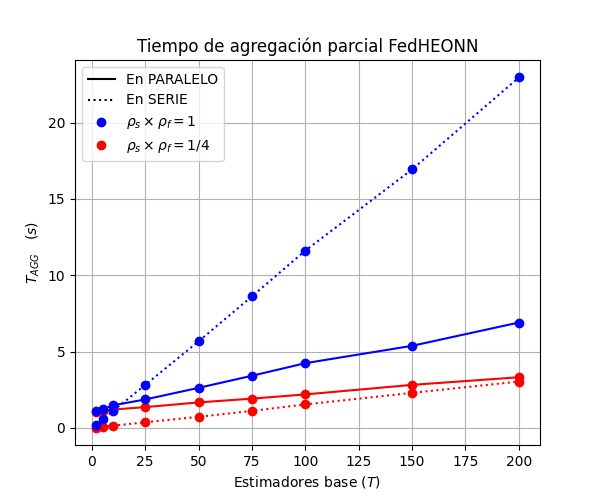
\includegraphics[width=\textwidth]{Figuras/tiempo_agg.png}
        \label{fig:par_agg1}
    \end{subfigure}
    \vfill
    \begin{subfigure}[b]{0.49\textwidth}
        \centering
        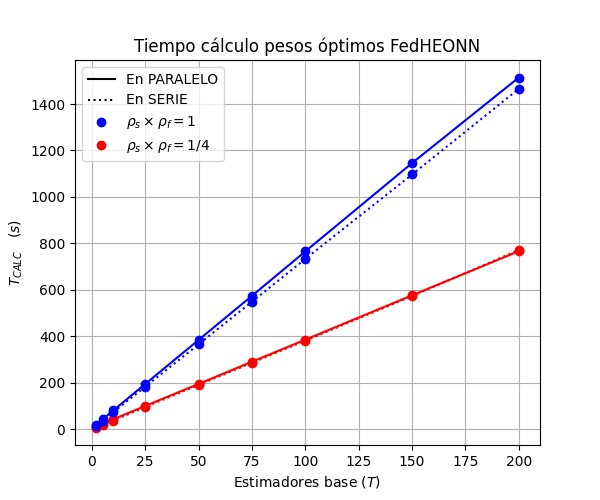
\includegraphics[width=\textwidth]{Figuras/tiempo_calc.png}
        \label{fig:par_calc1}
    \end{subfigure}
    \hfill
    \begin{subfigure}[b]{0.49\textwidth}
        \centering
        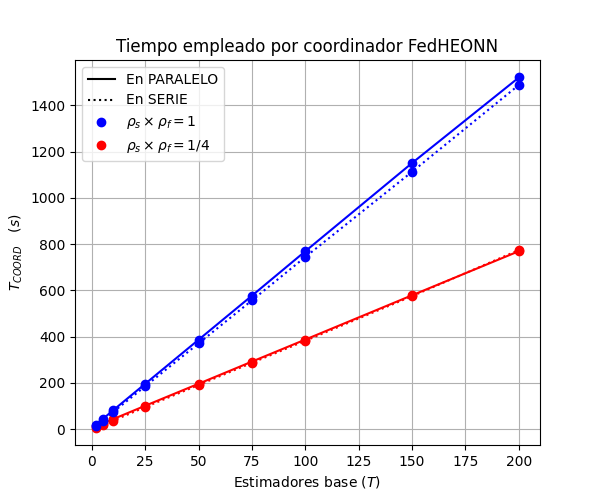
\includegraphics[width=\textwidth]{Figuras/tiempo_coord.png}
        \label{fig:par_coord1}
    \end{subfigure}
    \caption{Tiempos para las distintas tareas involucradas en FedHEONN}
    \label{fig:par_experiments}
\end{figure}

\vspace{0.5em}

 De estas podemos extraer varias conclusiones:
\begin{itemize}[noitemsep, topsep=2pt]
    \item La paralelización implementada es \textbf{efectiva en el entrenamiento de los clientes} (\texttt{fit}) y \textbf{la agregación parcial del coordinador} (\texttt{aggregate\_partial}), pero no lo es (por lo menos para el rango de estimadores base estudiados) en el cálculo de pesos óptimos (\texttt{calculate\_weights}).
    \item En la paralelización del cálculo de pesos óptimos, aún repartiendo el trabajo entre varios \textit{cores}, el sobrecoste de serializar y manipular vectores encriptados, realizar operaciones con ellos y crear \textit{pools} de procesos hace simplemente que \textbf{la implementación desarrollada para esta tarea no sea útil}.
    \item Como, a mayores, se trata de la tarea más lenta, la paralelización del coordinador apenas muestra alguna diferencia importante frente a la versión en serie ($T_{COORD} = T_{AGG} + T_{CALC}$).
    \item En cambio, para clientes con poca potencia computacional pero multi-núcleo, como algunos dispositivos embebidos, si que supone una ventaja importante frente a la versión original.
    \item La paralelización funcionó bien para aquellos procesos que paralelizaron las operaciones costosas sobre \textit{datos-en-claro}, por ejemplo la descomposición SVD, necesario en el \texttt{fit} y \texttt{aggregate\_partial}, y \textbf{no en donde hubo que trabajar con vectores encriptados}.
    \item Los resultados anteriores sugieren que la paralelización del entrenamiento en los clientes es favorable para todo $T$, mientras que la de la agregación parcial en el coordinador, solo lo es en casos con alto número de estimadores base $T$ y/o gran tamaño relativo $\rho_s\times\rho_f$, como se aprecia en la figura superior derecha de \ref{fig:par_experiments}, dando pie a un umbral{ }--{ }por determinar y específico de cada \textit{dataset}{ }--{}, a partir del cual compensa esta paralelización.
\end{itemize}


%TIEMPO GLOBAL T vs rho_p rho_s T y regla experimental, usar cuando rho_p rho_s T > nº cores%

\subsection{Prototipo desarrollado para el entorno federado}
La demostración realizada consistió en un portátil (Lenovo Y540) actuando como servidor/coordinador, con el otro (Lenovo X200) ejecutando dos clientes, todos conectados a la misma red doméstica.

Uno de estos clientes entrenará con la mitad de los datos de entrenamiento del \textit{dataset} $\bsym{X}_p$ y el otro con la parte restante. El primero que finalice su entrenamiento enviará su información al servidor, donde el coordinador la agregará y encolará la parte restante recibida mientras tanto. Una vez realizada la agregación incremental de ambas, y con la cola ya vacía, se calcularán los pesos óptimos, que se enviarán a uno de los clientes para que este realice una predicción sobre el conjunto de datos de \textit{test}.

La \textbf{demo} no se pudo realizar involucrando a los dispositivos Raspberry y Jetson Nano, tal y como se había planteado al principio, debido a que la librería necesaria para la encriptación homomórfica TenSEAL no está soportada bajo las arquitecturas ARM disponibles. En un futuro se espera que se soporten, pero de momento prescindimos de ellos en la red federada.

A continuación presentamos unas figuras mostrando diferentes momentos del entrenamiento federado, explicando brevemente que pasa en cada una de ellas:

% TODO FIGURAS PROCESO DEMO
\begin{figure}[H]
    \centering
    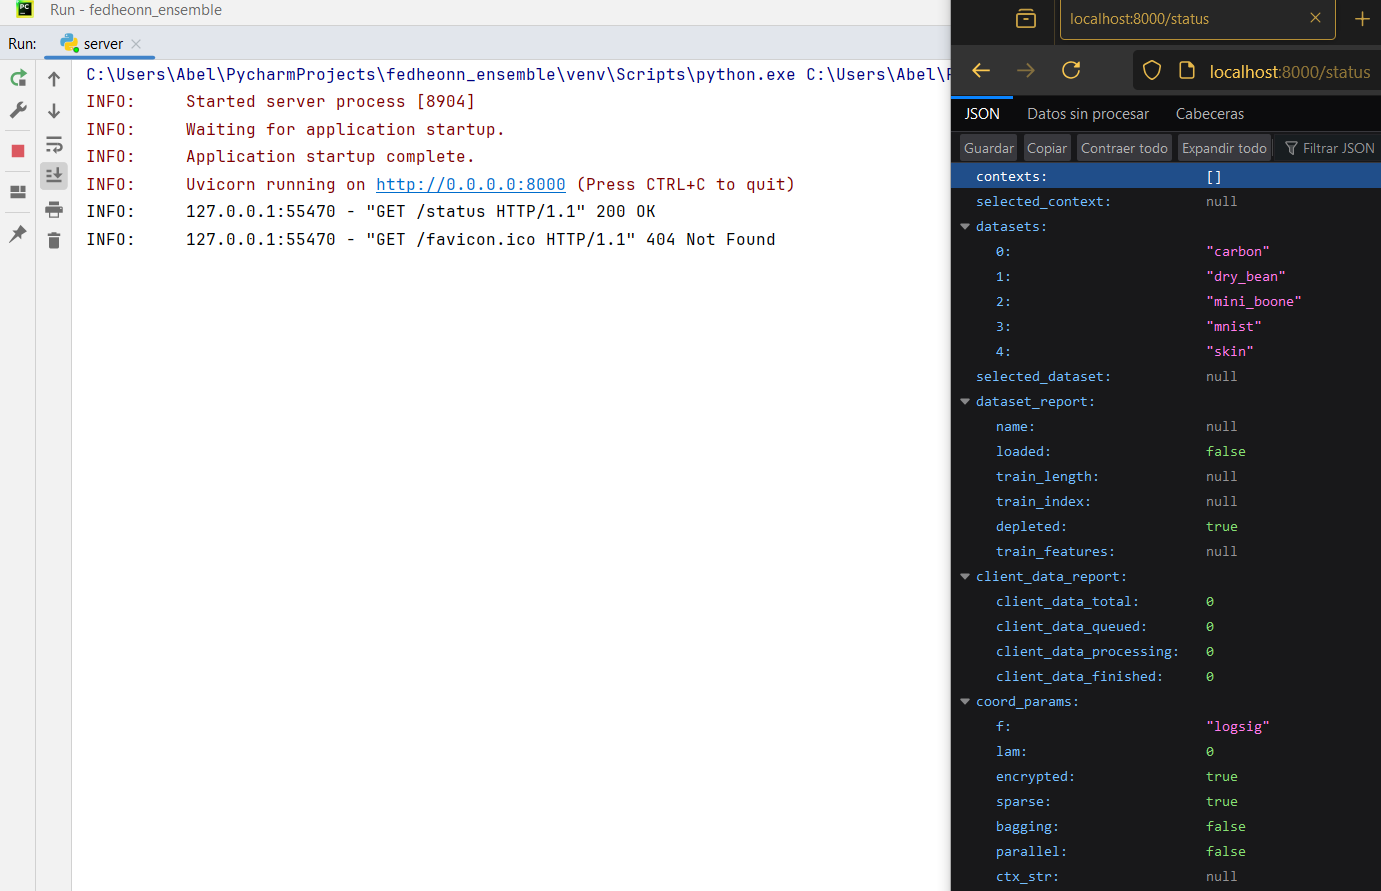
\includegraphics[width=.95\linewidth]{Figuras/server_1.png}
    \caption{Arranque del servidor.}
    \label{fig:srv_startup}
\end{figure}

\begin{figure}[H]
    \centering
    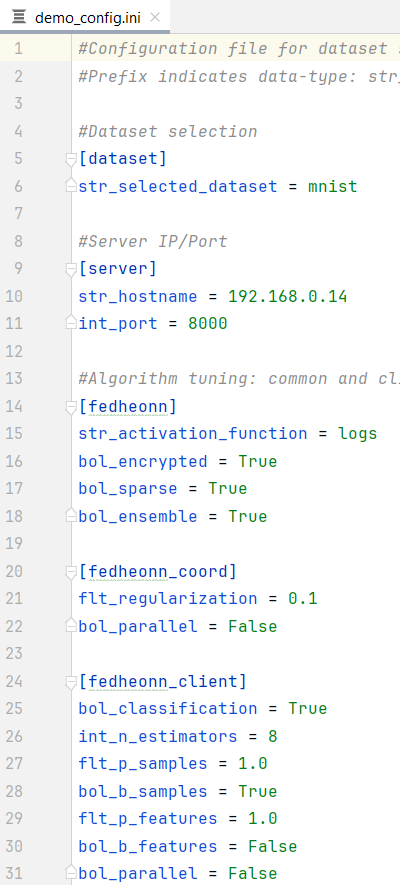
\includegraphics[scale=0.8]{Figuras/demo_config.png}
    \caption{Configuración utilizada durante la \textit{demo} para cliente y coordinador FedHEONN.}
    \label{fig:srv_config}
\end{figure}

\begin{figure}[H]
    \centering
    \begin{subfigure}[b]{\textwidth}
        \centering
        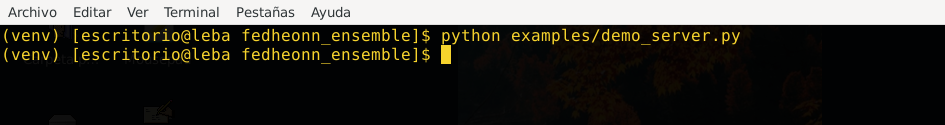
\includegraphics[width=\textwidth]{Figuras/demo_config_server.png}
    \end{subfigure}
    \vfill
    \begin{subfigure}[b]{\textwidth}
        \centering
        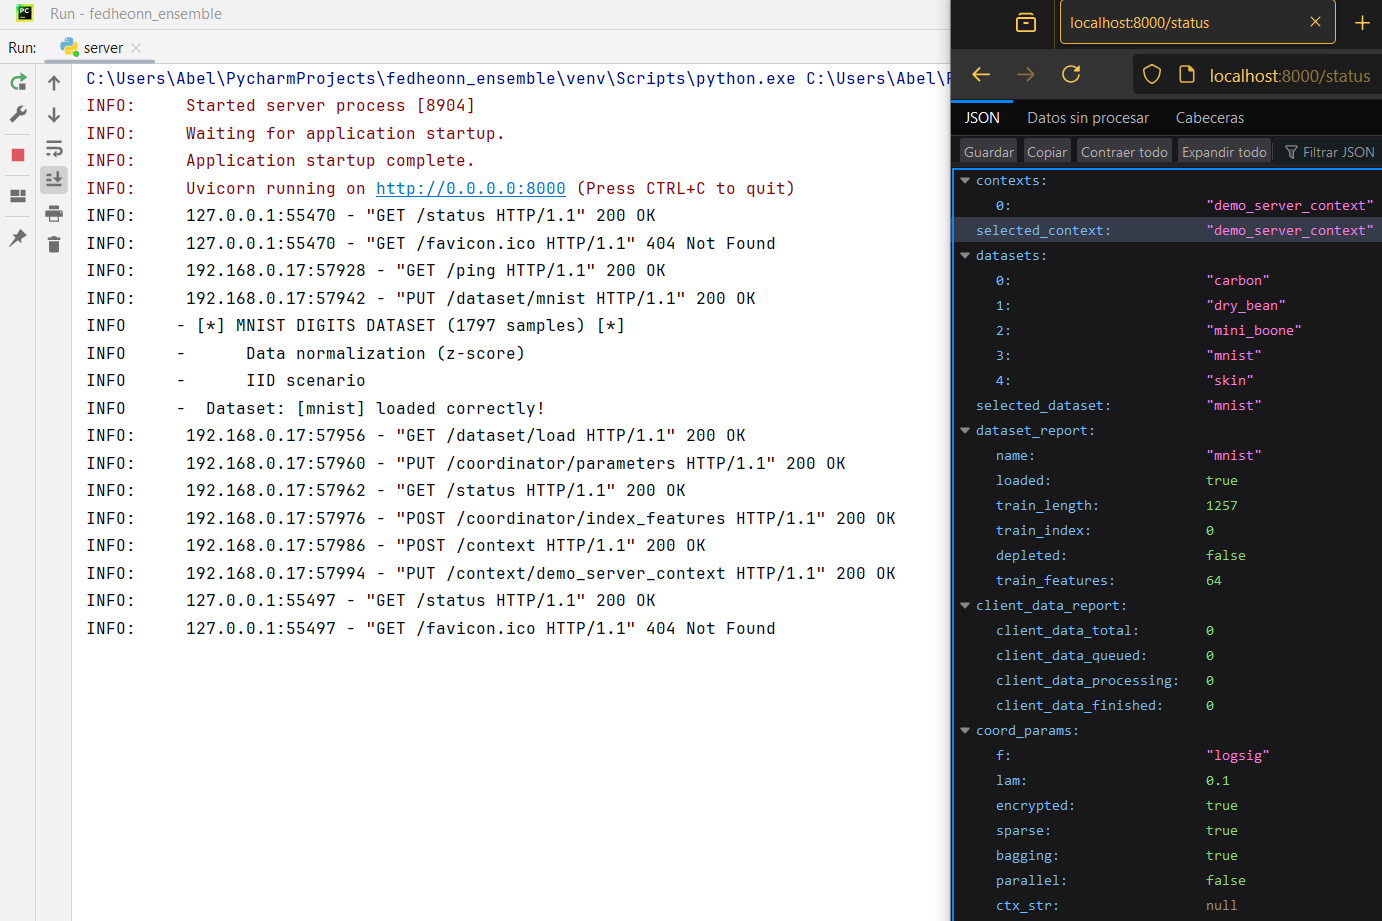
\includegraphics[width=\textwidth]{Figuras/server_2.png} 
    \end{subfigure}
    \caption{Ejecución de \texttt{demo\_server.py} y reflejo en el \textit{status} del servidor.}
    \label{fig:srv_setup}
\end{figure}

\begin{figure}[H]
    \centering
    \begin{subfigure}[b]{0.45\textwidth}
        \centering
        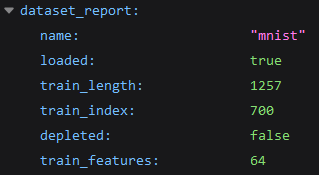
\includegraphics[width=\textwidth]{Figuras/server_3_client1.png}
        \caption{Primer cliente, obteniendo 700 registros.}
    \end{subfigure}
    \hspace{0.05\textwidth}
    \begin{subfigure}[b]{0.45\textwidth}
        \centering
        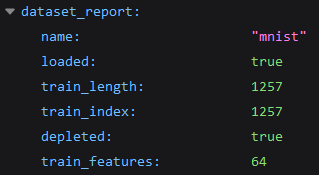
\includegraphics[width=\textwidth]{Figuras/server_3_client2.png}
        \caption{Segundo cliente, recogiendo los restantes.}
    \end{subfigure}
    \caption{Descarga de los datos del conjunto de entrenamiento desde el servidor.}
    \label{fig:server_dataset_load}
\end{figure}

%TODO TEXTO:
Hasta ahora hemos iniciado el servidor y configurado los parámetros del coordinador acoplado (figuras \ref{fig:srv_startup} y \ref{fig:srv_config}) mediante la ejecución de \verb|server.py| en un portátil y de \verb|demo_server.py| en el otro. A mayores, también se ha seleccionado el \textit{dataset} así como generado y subido el contexto público de TenSEAL al servidor (figura \ref{fig:srv_setup}).

\vspace{0.5em}

Seguidamente, en el portátil secundario se iniciarán dos instancias de \verb|demo_client.py|, programas que empiezan descargando los datos de entrenamiento del servidor, como se observa en las figuras \ref{fig:server_dataset_load} y \ref{fig:client_startup}, hasta que el \textit{dataset} se agota. Luego, empezamos el entrenamiento de ambos simultáneamente y esperamos a que, según acaben su \textit{entrenamiento local}, manden esta información al servidor para su agregación y cálculo de pesos óptimos (figura \ref{fig:client_train}).

\vspace{0.5em}

Como se ve en la figura \ref{fig:srv_queue}, el número de clientes conectados y procesados, así como la gestión de la cola de agregación, funciona como se había planteado en la sección \ref{sec:servidor_sol}. Por último, una vez finalizado el proceso de agregación y cálculo por parte del servidor, se reciben los pesos óptimos y se realiza una predicción sobre el conjunto de \textit{test} (figura \ref{fig:client_finished}).

\begin{figure}[H]
    \centering
    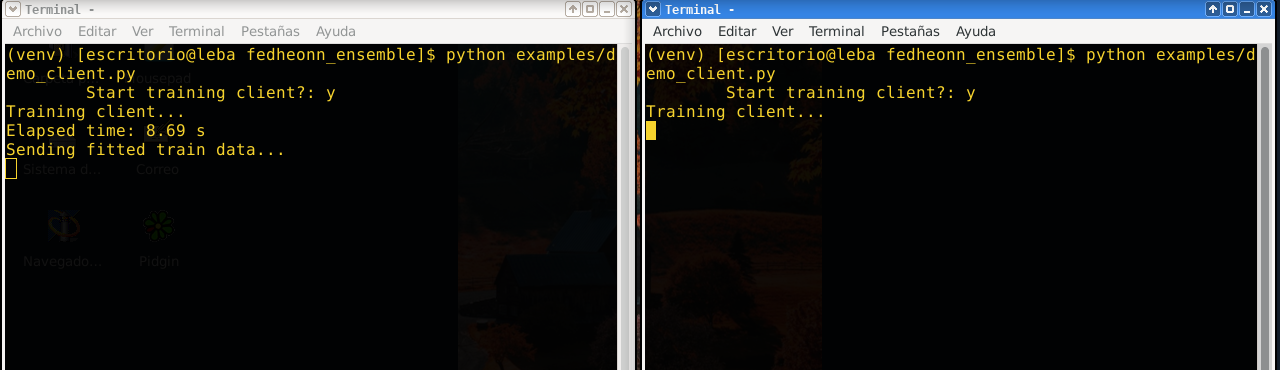
\includegraphics[width=\linewidth]{Figuras/c1.png}
    \caption{Arranque de los clientes.}
    \label{fig:client_startup}
\end{figure}

\begin{figure}[H]
    \centering
    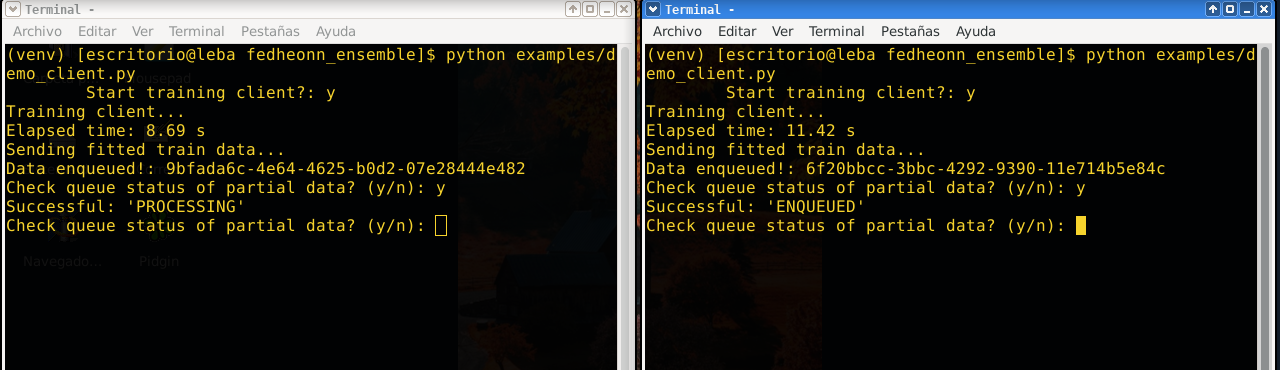
\includegraphics[width=\linewidth]{Figuras/c2.png}
    \caption{Comienzo del entrenamiento local en ambos clientes.}
    \label{fig:client_train}
\end{figure}

\begin{figure}[H]
    \centering
    \begin{subfigure}[b]{0.3\textwidth}
        \centering
        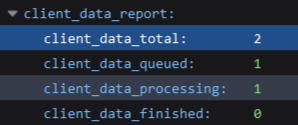
\includegraphics[width=\textwidth]{Figuras/server_clients1.png}
        \caption{Agregando primer lote.}
    \end{subfigure}
    \hspace{0.03\textwidth}
    \begin{subfigure}[b]{0.3\textwidth}
        \centering
        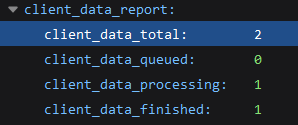
\includegraphics[width=\textwidth]{Figuras/server_clients2.png}
        \caption{Agregando segundo lote.}
    \end{subfigure}
     \hspace{0.03\textwidth}
    \begin{subfigure}[b]{0.3\textwidth}
        \centering
        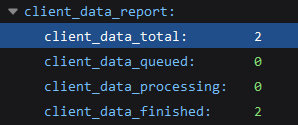
\includegraphics[width=\textwidth]{Figuras/server_clients3.png}
        \caption{Clientes procesados.}
    \end{subfigure}
    \caption{Funcionamiento de la cola de agregación en el servidor.}
    \label{fig:srv_queue}
\end{figure}

\begin{figure}[H]
    \centering
    \begin{subfigure}[b]{\textwidth}
        \centering
        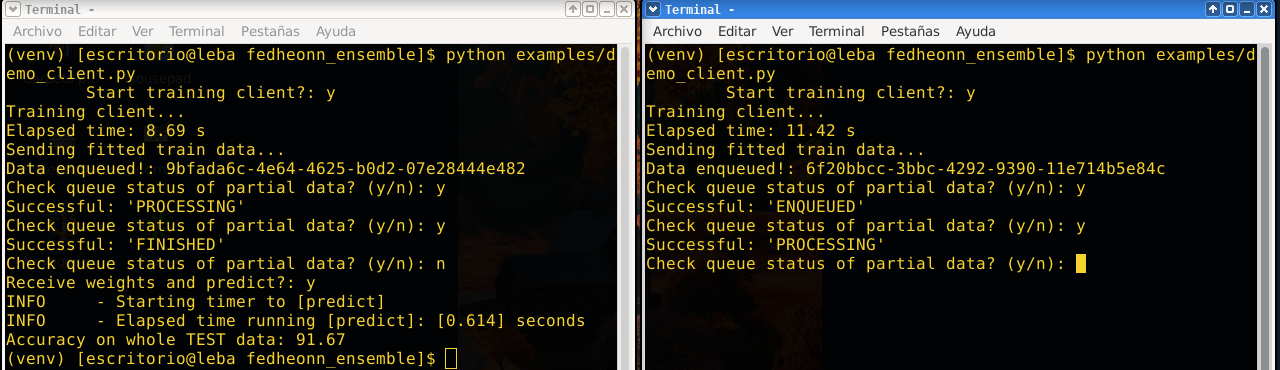
\includegraphics[width=\textwidth]{Figuras/c3.png}
    \end{subfigure}
    \vfill
    \begin{subfigure}[b]{\textwidth}
        \centering
        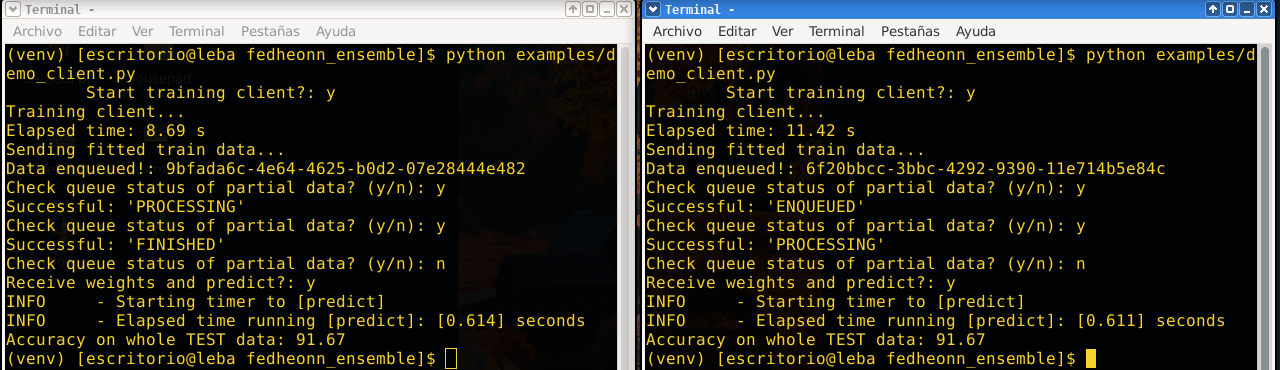
\includegraphics[width=\textwidth]{Figuras/c4.png} 
    \end{subfigure}
    \caption{Finalización de ambos clientes con predicción sobre \textit{test}.}
    \label{fig:client_finished}
\end{figure}

\subsection{Eficiencia: emisiones y consumo energético} \label{sec:res_eficiencia}
Terminamos este capítulo presentando los distintos experimentos realizados integrando la herramienta \textit{CodeCarbon} directamente en el código de los modelos presentados hasta ahora y en otros equivalentes, para realizar una comparativa en cuanto a consumo energético y eficiencia.

\vspace{0.5em}

En el primer experimento, correspondiente al fichero \verb|codecarbon_mnist_incremental.py| del directorio \verb|examples|, comparamos el modelo original contra su versión con ensamblaje y contra un tipo de RNA denominada \textit{perceptrón multicapa} (MLPC), realizando el entrenamiento de modo \textbf{incremental}; obteniendo el gasto energético, su desglose para cada proceso y las métricas finales resultantes, utilizando el conjunto de datos \textit{MNIST-simp}.

\vspace{0.5em}

Se divide el conjunto de datos de entrenamiento y se ejecuta el programa con un determinado número de clientes $P$ y clientes por grupo $N_g$. Para imitar un agregado incremental en el MLPC, simplemente realizamos su \textit{fit} con la sucesiva unión de las submatrices $\bsym{X}_p$. Para ser justos con el modelo FedHEONN, durante la primera prueba desactivamos la encriptación para no añadir costes computacionales que el MLPC tampoco considera, y la activamos, por comparación, en la segunda.

En la tabla \ref{tab:hiperparam_cc_inc1_mlpc} se resumen los hiperparámetros utilizados para estas dos pruebas y en las tablas \ref{tab:resultados_ccmnist_inc1} y \ref{tab:resultados_ccmnist_inc2} los resultados obtenidos con estas:

%TODO TABLA HIPERPARAM
\begin{table}[H]
\centering
\begin{tabular}{@{}rcccccccccc@{}}
\toprule
\multicolumn{1}{r}{\texttt{MNIST-simp}} & $\bsym{P}$ & $\bsym{N}_g$ & \textbf{Encript.} & $\bsym{\lambda}$ & \textbf{F.act.} & $\bsym{T}$ & $\bsym{\rho}_s$ & $\bsym{\beta}_s$ & $\bsym{\rho}_f$ & $\bsym{\beta}_f$ \\ \midrule
FedHEONN              & 2          & 1    & X        & 10              & \textit{logsig}         & -          & -             & -            & -              & -            \\
FedHEONN              & 2          & 1    & \checkmark        & 10              & \textit{logsig}         & -          & -             & -            & -              & -            \\
FedHEONN\_ensemble     & 2          & 1  & X           & 0.1             & \textit{logsig}         & 25         & 0.2           & $\checkmark$         & 1              & X        \\
FedHEONN\_ensemble     & 2          & 1  & \checkmark           & 0.1             & \textit{logsig}         & 25         & 0.2           & $\checkmark$         & 1              & X        \\ \bottomrule
\end{tabular}

\vspace{1cm}

\begin{tabular}{@{}rcccccccc@{}}
\toprule
 \texttt{MNIST-simp} & $\bsym{P}$ & $\bsym{N}_g$ & \textbf{F.act.} & $\bsym{\lambda}$ & \textbf{Max.Iter.} & \textbf{Tol.} & \textbf{Solver} & \textbf{Capas ocultas} \\ \midrule
\multicolumn{1}{r}{MLPC} & 2          & 1            & \textit{relu}            & 0.0001         & 500               & 0.0001       & SGD             & $(128,\, 64)$              \\ \bottomrule
\end{tabular}

\caption{Hiperparámetros ejecutados en \texttt{codecarbon\_mnist\_incremental.py}.}

\label{tab:hiperparam_cc_inc1_mlpc}
\end{table}

%TODO TABLA RESULTADOS
\begin{table}[H]
\centering
\resizebox{\textwidth}{!}{
\begin{tabular}{@{}crllcc@{}}
\toprule
\multicolumn{2}{c}{\texttt{MNIST-simp}} &
  \textbf{Energía cons. (kWh)} &
  \textbf{Emisiones ($CO_2^{eq}$ kg)} &
  \multicolumn{1}{l}{\textbf{Duración (s)}} &
  \multicolumn{1}{l}{\textbf{Exactitud (\%)}} \\ \midrule
\multicolumn{2}{r}{\textbf{FedHEONN}} &
  \multicolumn{1}{r}{\textbf{3.5349E-06}} &
  \multicolumn{1}{r}{\textbf{7.6857E-07}} &
  \textbf{14.79} &
  \textbf{91.70} \\
T & \texttt{fit\_group\_1}                & 1.5570E-06 & 3.3853E-07 & 2.70  & -     \\
A & \texttt{aggregate\_partial\_group\_1}  & 1.0925E-07 & 2.3753E-08 & 2.33  & -     \\
R & \texttt{calc\_optim\_weights\_group\_1} & 8.6960E-08 & 1.8907E-08 & 2.37  & 90.92 \\
E & \texttt{fit\_group\_2}                & 1.5713E-06 & 3.4163E-07 & 2.69  & -     \\
A & \texttt{aggregate\_partial\_group\_2}  & 1.3059E-07 & 2.8394E-08 & 2.37  & -     \\
S & \texttt{calc\_optim\_weights\_group\_2} & 7.9835E-08 & 1.7358E-08 & 2.33  & 91.70 \\
\multicolumn{2}{r}{\textbf{FedHEONN\_ensemble}} &
  \multicolumn{1}{r}{\textbf{5.4776E-05}} &
  \multicolumn{1}{r}{\textbf{1.1910E-05}} &
  \textbf{28.07} &
  \textbf{93.71} \\
T & \texttt{fit\_group\_1}                & 2.2291E-05 & 4.8467E-06 & 7.94  & -     \\
A & \texttt{aggregate\_partial\_group\_1}  & 3.1480E-06 & 6.8445E-07 & 3.13  & -     \\
R & \texttt{calc\_optim\_weights\_group\_1} & 2.2596E-06 & 4.9129E-07 & 2.94  & 93.53 \\
E & \texttt{fit\_group\_2}                & 2.0662E-05 & 4.4924E-06 & 7.75  & -     \\
A & \texttt{aggregate\_partial\_group\_2}  & 4.0839E-06 & 8.8792E-07 & 3.40  & -     \\
S & \texttt{calc\_optim\_weights\_group\_2} & 2.3316E-06 & 5.0694E-07 & 2.91  & 93.71 \\
\multicolumn{2}{r}{\textbf{MLPC}} &
  \multicolumn{1}{r}{\textbf{1.7256E-04}} &
  \multicolumn{1}{r}{\textbf{3.7519E-05}} &
  \textbf{45.32} &
  \textbf{97.27} \\
T & \texttt{fit\_group\_1}                & 7.0460E-05 & 1.5320E-05 & 18.22 & 96.62 \\
. & \texttt{fit\_group\_2}                & 1.0210E-04 & 2.2199E-05 & 27.10 & 97.27 \\ \bottomrule
\end{tabular}
}
\caption{Desglose por tareas y modelo del consumo energético, emisiones, duración y exactitud de la primera prueba (\textbf{sin encriptación}).}
\label{tab:resultados_ccmnist_inc1}
\end{table}

\begin{table}[ht]
\centering
\resizebox{\textwidth}{!}{
\begin{tabular}{@{}crllcc@{}}
\toprule
\multicolumn{2}{c}{\texttt{MNIST-simp}} &
  \textbf{Energía cons. (kWh)} &
  \textbf{Emisiones ($CO_2^{eq}$ kg)} &
  \multicolumn{1}{l}{\textbf{Duración (s)}} &
  \multicolumn{1}{l}{\textbf{Exactitud (\%)}} \\ \midrule

\multicolumn{2}{r}{\textbf{FedHEONN}} &	  \multicolumn{1}{r}{\textbf{2.3780E-04}} & \multicolumn{1}{r}{\textbf{5.1703E-05}} & \textbf{49.37} & \textbf{91.70} \\
T & \texttt{fit\_group\_1}                	& 5.5734E-06	& 1.2118E-06 	& 3.00  & -     \\
A & \texttt{aggregate\_partial\_group\_1}  	& 2.2911E-07 	& 4.9814E-08 	& 2.33  & -     \\
R & \texttt{calc\_optim\_weights\_group\_1} & 1.1696E-04 	& 2.5430E-05 	& 19.41  & 90.92 \\
E & \texttt{fit\_group\_2}                	& 4.3034E-06	& 9.3565E-07 	& 2.96  & -     \\
A & \texttt{aggregate\_partial\_group\_2}  	& 4.1601E-07 	& 9.0449E-08 	& 2.36  & -     \\
S & \texttt{calc\_optim\_weights\_group\_2} & 1.1032E-04 	& 2.3985E-05 	& 19.32  & 91.70 \\

\multicolumn{2}{r}{\textbf{FedHEONN\_ensemble}} &  \multicolumn{1}{r}{\textbf{5.8543E-03}} &  \multicolumn{1}{r}{\textbf{1.2728E-03}} &  \textbf{885.20} & \textbf{93.71} \\
T & \texttt{fit\_group\_1}                	& 1.3924E-04 & 3.0274E-05 & 17.74  & -     \\
A & \texttt{aggregate\_partial\_group\_1}  	& 6.0752E-06 & 1.3209E-06 & 3.22  & -     \\
R & \texttt{calc\_optim\_weights\_group\_1} & 3.1583E-03 & 6.8668E-04 & 421.00  & 93.53 \\
E & \texttt{fit\_group\_2}                	& 1.1635E-04 & 2.5296E-05 & 16.64  & -     \\
A & \texttt{aggregate\_partial\_group\_2}  	& 1.2313E-05 & 2.6770E-06 & 3.74  & -     \\
S & \texttt{calc\_optim\_weights\_group\_2} & 2.4220E-03 & 5.2659E-04 & 422.86  & 93.71 \\

\multicolumn{2}{r}{\textbf{MLPC}} &  \multicolumn{1}{r}{\textbf{3.1616E-04}} & \multicolumn{1}{r}{\textbf{6.8739E-05}} & \textbf{45.01} & \textbf{97.27} \\
T & \texttt{fit\_group\_1}                & 1.3565E-04 & 2.9494E-05 & 19.22 & 96.62 \\
. & \texttt{fit\_group\_2}                & 1.8051E-04 & 3.9246E-05 & 25.79 & 97.27 \\ \bottomrule
\end{tabular}
}
\caption{Desglose por tareas y modelo del consumo energético, emisiones, duración y exactitud de la segunda prueba (\textbf{con encriptación}).}
\label{tab:resultados_ccmnist_inc2}
\end{table}

Los ficheros originales se pueden encontrar en la carpeta \verb|emissions_results| del directorio \verb|examples|. Para implementar el MLPC se usó la librería \textit{scikit-learn}.

Como cabría esperar, la energía consumida por el modelo bajo ensamblaje es mayor que el original, y a su vez, el del MLPC es mayor que ambos. El incremento en el consumo de la versión original a la versión con ensamblaje es de \textbf{un orden de magnitud mayor}, pasando de unos $3.5\times 10^{-6}$ a $5.5\times 10^{-5}\;kWh$ respectivamente.

Cuando se activa la encriptación, para sendas versiones, se produce un incremento en el consumo energético de \textbf{dos ordenes de magnitud}, pasando, aproximadamente, de $3.5\times 10^{-6}$ a $2.4\times 10^{-4}\;kWh$ para el modelo original y de $5.5\times 10^{-5}$ a $5.8\times 10^{-3}\;kWh$ para la versión con ensamblaje (resultados para \verb|FedHEONN| y \verb|FedHEONN_ensemble| de las tablas \ref{tab:resultados_ccmnist_inc1} y \ref{tab:resultados_ccmnist_inc2}).

Cabe destacar cómo solo es este último caso, FedHEONN encriptado con ensamblaje, el que consume más energía que el modelo MLPC ensayado ($3.2\times 10^{-4}\;kWh$), unas 18 veces más. Con todo, en estas pruebas estamos comparados modelos con su conjunto de hiperparámetros ya ajustado, mientras que una prueba más realista incluiría también el tiempo y consumo energético resultante de dicho ajuste (por ejemplo, mediante \textit{grid search}). Teniendo en cuenta lo anterior, y como el modelo FedHEONN presenta un solo hiperparámetro en su versión original (la \textit{regularización} $\lambda$), y otros tres más si hacemos uso del ensamblaje (el número de estimadores base ${T}$ y el tamaño relativo del parche, ${\rho}_s$ y ${\rho}_f$), cabe esperar que el \textbf{consumo energético global de su ajuste sea menor} que para el caso del MLPC u otras RNA, ya que presentan un abanico mucho mayor y más abierto de hiperparámetros y diseños (número de capas, número de neuronas por capa, funciones de activación, regularización, etc.).

Al mismo tiempo también podemos observar, en el desglose de tareas, que, \textbf{cuando no se usa la encriptación}, el entrenamiento en los clientes es el proceso que más consume, seguido de la agregación y el cálculo de pesos óptimo, debido a que los dos primeros involucran descomposiciones en valores singulares (SVD), además de otras operaciones, y la última solo unas pocas multiplicaciones de matrices.

En cambio, \textbf{cuando se usa la encriptación}, el orden es el inverso, siendo el entrenamiento y agregación las tareas más livianas y la multiplicación de matrices y vectores encriptados, necesarios para el cálculo de pesos óptimos, la más pesada de todas.

\vspace{1em}

En el último experimento, correspondiente al \verb|codecarbon_mnist_experiments.py|, comparamos la \textbf{versión original} de FedHEONN, con y sin encriptación (referidos como \verb|FedHEONN| y \verb|FedHEONN_enc|), la \textbf{versión con ensamblaje}, usando la mejor combinación de $\rho_s\,\times\,\rho_f$ vista en la sección \ref{sec:result_ensamblaje}, otra alternativa de menor tamaño relativo (denominados \verb|FedHEONN_ensemble| y \verb|FedHEONN_ensemble_alt| respectivamente), y el \textbf{modelo de MLPC} implementado con \textit{scikit-learn}. Los ejecutamos sobre todos los conjuntos de datos de tipo MNIST presentados en la tabla \ref{tab:datasets}; a saber, \textit{MNIST-orig}, \textit{MNIST-simp} y \textit{MNIST-test}.

De nuevo, la configuración de los hiperparámetros utilizada se resume en la tabla \ref{tab:hiperparam_cc_exp_fedheon} y los resultados obtenidos en la tabla \ref{tab:resultados_ccmnist_exp}:

%TODO TABLA HIPERPARAM
\begin{table}[H]
\centering

\begin{tabular}{@{}lcccccccc@{}}
\toprule
& $\bsym{P}$ & \textbf{F.act.} & $\bsym{\lambda}$ & \textbf{Max.Iter.} & \textbf{Tol.} & \textbf{Solver} & \textbf{Capas ocultas} \\ \midrule
\multicolumn{1}{r}{MLPC} & 1   & \textit{relu}    & 0.0001     & 500       & 0.0001       & SGD      & $(128,\, 64)$           \\ \bottomrule
\end{tabular}

\vspace{1cm}

\begin{tabular}{@{}rccccccccc@{}}
\toprule
& $\bsym{P}$ & \textbf{Encript.} & \textbf{F.act.} & $\bsym{\lambda}$ & $\bsym{T}$ & $\bsym{\rho}_s$ & $\bsym{\beta}_s$ & $\bsym{\rho}_f$ & $\bsym{\beta}_f$ \\ \midrule
FedHEONN              & 1          & X            & \textit{logsig}              & 10         & -          & -             & -            & -              & -            \\
FedHEONN\_enc              & 1          & \checkmark            & \textit{logsig}              & 10        & -          & -             & -            & -              & -            \\
FedHEONN\_ensemble     & 1    & X      & \textit{logsig}            & 0.01          & 75         & 0.2           & $\checkmark$         & 0.8              & X        \\
FedHEONN\_ensemble\_alt     & 1    & X       & \textit{logsig}            & 0.1          & 25         & 0.2           & $\checkmark$         & 1              & X        \\ \bottomrule
\end{tabular}
\caption{Hiperparámetros de los modelos en \texttt{codecarbon\_mnist\_experiments.py}.}
\label{tab:hiperparam_cc_exp_fedheon}
\end{table}

%TODO TABLA RESULTADOS
\begin{table}[H]
\centering
\resizebox{\textwidth}{!}{
\begin{tabular}{@{}rrrcc@{}}
\toprule
\multicolumn{1}{c}{\texttt{MNIST-test}} &
  \textbf{Energía cons. (kWh)} &
  \textbf{Emisiones ($CO_2^{eq}$ kg)} &
  \multicolumn{1}{l}{\textbf{Duración (s)}} &
  \multicolumn{1}{l}{\textbf{Precisión (\%)}} \\ \midrule
\textbf{FedHEONN}               & \multicolumn{1}{r}{1.9533E-06} & \multicolumn{1}{r}{4.2468E-07} & 2.68                 & 90.74                \\
\textbf{FedHEONN\_enc}           & \multicolumn{1}{r}{3.4259E-04} & \multicolumn{1}{r}{7.4486E-05} & 13.84                & 90.74                \\
\textbf{FedHEONN\_ensemble}      & \multicolumn{1}{r}{1.4024E-04} & \multicolumn{1}{r}{3.0491E-05} & 13.75                & 95.19                \\
\textbf{FedHEONN\_ensemble\_alt}  & \multicolumn{1}{r}{7.8264E-05} & \multicolumn{1}{r}{1.7016E-05} & 8.52                 & 94.26                \\
\textbf{MLPC}                  & \multicolumn{1}{r}{1.2083E-04} & \multicolumn{1}{r}{2.6270E-05} & 13.38                & 97.41                \\ \midrule
\multicolumn{1}{c}{\texttt{MNIST-simp}} & \multicolumn{1}{l}{} & \multicolumn{1}{r}{} & \multicolumn{1}{r}{} & \multicolumn{1}{l}{} \\ \midrule
\textbf{FedHEONN}               & 2.4421E-06                     & 5.3097E-07                     & 2.86                 & 91.70                \\
\textbf{FedHEONN\_enc}           & 1.4766E-04                     & 3.2104E-05                     & 17.01                & 91.70                \\
\textbf{FedHEONN\_ensemble}      & 2.1581E-04                     & 4.6922E-05                     & 25.87                & 93.53                \\
\textbf{FedHEONN\_ensemble\_alt}  & 1.1547E-04                     & 2.5106E-05                     & 12.60                & 93.42                \\
\textbf{MLPC}                  & 2.5489E-04                     & 5.5420E-05                     & 26.81                & 97.27                \\ \midrule
\multicolumn{1}{c}{\texttt{MNIST-orig}} & \multicolumn{1}{l}{} & \multicolumn{1}{l}{} & \multicolumn{1}{l}{} & \multicolumn{1}{l}{} \\ \midrule
\textbf{FedHEONN}               & 1.6206E-03                     & 3.5236E-04                     & 132.37               & 81.30                \\
\textbf{FedHEONN\_enc}           & 3.4126E-03                     & 7.4198E-04                     & 352.99               & 81.32                \\
\textbf{MLPC}                  & 2.3676E-03                     & 5.1476E-04                     & 319.27               & 97.14                \\ \bottomrule
\end{tabular}
}
\caption[Consumo energético en experimento \texttt{codecarbon\_mnist\_experiments.py}]{Consumo energético, emisiones, duración y exactitud del experimento \texttt{codecarbon\_mnist\_experiments.py}.}
\label{tab:resultados_ccmnist_exp}
\end{table}

De estos últimos resultados destacamos las siguientes observaciones:

\begin{itemize}[topsep=2pt, itemsep=2pt]
    \item Tomando el modelo \textbf{FedHEONN sin encriptar} como base, el uso de la encriptación supone un coste computacional y, por tanto, energético, muy considerable, con un incremento de alrededor del \textbf{112 \%} en el mejor de los casos, pasando de $1.6\times10^{-3}$ a $3.4\times10^{-3}\;kWh$, en el escenario del \textit{dataset} más grande, \textit{MNIST-orig}, hasta un \textbf{17795 \%} para el más pequeño, \textit{MNIST-test}, pasando de $1.9\times10^{-6}$ a $3.4\times10^{-4}\;kWh$.

    \item La gran diferencia en el impacto energético de uno y otro caso, debido al uso o no de la encriptación, nos sugiere que \textbf{existe un bagaje considerable} por culpa de las operaciones realizadas con los vectores criptográficos y requeridas por el modelo; tanto que para \textit{datasets} pequeños, suponen costes computacionales incluso mayores a los inherentes al modelo FedHEONN sin encriptación.

    \item Por otro lado, el uso del \textbf{ensamblaje} también supone, como es evidente, un mayor consumo, al ser necesario entrenar múltiples estimadores base ${T}$; con todo, permite un mayor equilibrio entre eficacia y eficiencia, mediante el debido ajuste de sus parámetros.

    \item Por ejemplo, el incremento de hasta más de un \textbf{4 \%} en la exactitud bajo \textit{MNIST-test} con la mejor versión de ensamblaje, \verb|FedHEON_ensemble|, consume un \textbf{7500 \%} más ($1.4\times10^{-4}\;kWh$) que la versión original ($1.9\times10^{-6}\;kWh$), pero la versión alternativa, \verb|FedHEON_ensemble_alt|, de menor número de estimadores base $T$, obtiene una eficacia similar con \textit{solo} el \textbf{4000 \% }más de consumo ($7.8\times10^{-5}\;kWh$). Aunque ambos son incrementos sustanciales respecto a la versión original de referencia, la versión alternativa consume aproximadamente la mitad que la otra, siendo una opción mucho más \textbf{eficiente}.
\end{itemize}

\vspace{0.5em}

Por último, el modelo MLPC destaca por su alta exactitud y bajo consumo frente a las versiones encriptada y con ensamblaje pero sin encriptar de nuestro modelo ejecutadas para estas pruebas.

Siguen siendo, con todo, aún más costosas que la versión original de FedHEONN sin encriptación, aunque este obtenga métricas bastante peores. Sin embargo, la comparación no es del todo justa, ya que la versatilidad de uno y otro tipo de modelo también es distinta; y mientras \textbf{FedHEONN} permite un entrenamiento distribuido, incremental, federado e incluso bajo clientes con conjuntos de datos no IID, ninguna de estas capacidades aplican al otro modelo (MLPC), ni tampoco permite preservar la privacidad de los datos - mediante encriptación u otro tipo de técnica - si no que necesita centralizarlos.

\newpage

\section{Conclusiones y futuros trabajos}
Por último se trazarán escuetamente las conclusiones del proyecto y posibles líneas de trabajo.

\subsection{Conclusiones}
Demostrada la viabilidad del algoritmo presentado bajo escenarios realistas de entornos federados, las mejoras planteadas en este trabajo han sido implementadas obteniendo resultandos mayoritariamente satisfactorios, cuyo resumen listamos a continuación:

\begin{itemize}[topsep=2pt, itemsep=2pt]
    \item Se ha probado y mejorado la \textbf{naturaleza incremental} del algoritmo FedHEONN mediante su desglose en tareas de agregación parcial y cálculo de pesos óptimos en lotes, obteniendo los mismos resultados. Dicho desglose es útil, puesto que la agregación de la información recopilada es un proceso mucho menos costoso que el cálculo de los pesos finales, y se trata de una configuración más realista en un entorno federado en donde no todos los clientes pueden estar disponibles a la vez.
    \item Se ha incrementado la \textbf{capacidad de representación} del modelo mediante la incorporación de la técnica de \textit{ensemble} conocida como Random Patches, obteniendo mejoras notables en las métricas de reconocidos conjuntos de datos usados como \textit{benchmarks}.
    \item En un intento de \textbf{reducción de los tiempos globales} de entrenamiento con ensamblaje, se ha llevado a cabo la paralelización de las tareas de entrenamiento (\textit{cliente}) y agregación parcial y cálculo de pesos óptimos (\textit{coordinador}), con y sin encriptación, resultando en procesos más rápidos bajo determinados escenarios.
    \item El \textit{sobrecoste} añadido por el manejo y creación de procesos, así como la serialización y reconstrucción de vectores encriptados hicieron que las anteriores tareas solo compensen su paralelización para un \textbf{alto número de estimadores base} $\bsym{T}$.
    \item El \textit{sobrecoste} de la serialización y reconstrucción de vectores criptográficos es un factor importante y un coste computacional añadido a tener en cuenta también para el prototipo de entorno federado desarrollado, al que se une el hecho de que la librería de encriptación homomórfica elegida no soporte actualmente dispositivos embebidos bajo arquitectura ARM, frustrando alguno de los experimentos de este trabajo.
    \item El análisis de los consumos energéticos del modelo original con el ensamblaje y otros semejantes nos permitió: \textbf{cuantificar y ejemplificar} muchos de los aspectos tratados en el apartado de IA verde/roja (sección \ref{ss:green_ia}), en cuanto a eficacia y eficiencia; y, por otro, \textbf{desglosar el consumo de las tareas} involucradas en el proceso federado de FedHEONN, así como el uso{ }--{ }o no{ }--{ }de la encriptación durante el mismo.
\end{itemize}

\subsection{Futuros trabajos}
En cuanto a futuros trabajos de investigación a los que da pie el modelo presentado, podemos destacar:
\begin{itemize}[topsep=2pt, itemsep=2pt]
    \item Hacer uso de alguna otra librería de encriptación homomórfica, como \href{https://github.com/ibarrond/Pyfhel}{\textit{Pyfhel}}, para \textbf{comparar rendimientos} en las operaciones con vectores y multiplicación de matrices encriptados, así como con la serialización y reconstrucción de los mismos y de sus contextos asociados. Comprobar que \textbf{soporten dispositivos embebidos} con arquitectura ARM, como las Raspberry mencionadas en este trabajo, o esperar a que TenSEAL lo haga.
    \item Integrar la librería de \href{https://github.com/google/jax}{\textit{Google Jax}} en el proyecto con el objeto de \textbf{acelerar las descomposiciones en valores singulares} (SVD), que son vitales en la agregación de información (\textit{coordinador}) y entrenamiento (\textit{clientes}), ejecutándolos en entornos con TPU's, como pueden ser \href{https://cloud.google.com/tpu?hl=es-419}{\textit{Google Cloud TPU}} para la coordinación y Raspberry's con coprocesadores \href{https://coral.ai/products/}{\textbf{Coral}} como clientes.
    \item Realizar una \textbf{comparativa con otros modelos federados} de uso actual, para ver si FedHEONN es más eficiente solo en términos de rondas de comunicación de información necesarias para su entrenamiento o si también en el propio consumo energético requerido por el mismo.
    \item Acoplar este modelo a otros algoritmos federados de características semejantes para producir una combinación más potente y con una \textbf{capacidad de representación más compleja}.
    \item La elaboración de una \textbf{técnica inteligente específica para el ajuste de los hiper-parámetros utilizados en Random Patches}. Probando diferentes extremos de los posibles tamaños relativos de los parches, $\rho_s \times \rho_f \in (0,\,1)$, se puede ir precisando y encontrando los valores que generan mejores métricas finales de un modo más óptimo que realizando una bruta búsqueda en cuadricula.
\end{itemize}

\newpage

\section{Referencias}
En este capítulo disponemos las referencias de los distintos recursos empleados en este Trabajo Final de Grado.

\subsection{Bibliografía}
A continuación listamos los libros, revistas, artículos científicos, páginas web u otro tipo de publicaciones considerados de interés y citados en la memoria:

\bibliographystyle{plain}
\bibliography{Bibliografia}

\subsection{Otras referencias}\label{sec:documentacion}

En este apartado reflejamos todos aquellos manuales que hemos consultado durante la configuración, uso e implementación, tanto de los distintos dispositivos físicos empleados (\textit{hardware}), como durante el desarrollo de los métodos y técnicas descritas para modelo (\textit{software}):

\begin{itemize}[itemsep=2pt]
    \item \textbf{Raspberry Pi 4 Product Brief}, PDF disponible en \url{https://datasheets.raspberrypi.com/rpi4/raspberry-pi-4-product-brief.pdf}
    \item \textbf{Raspberry Pi Official Getting Started Guide}, consulta disponible en \url{https://www.raspberrypi.com/documentation/computers/getting-started.html}
    \item \textbf{Raspberry Pi Official Documentation}, consulta disponible en \url{https://www.raspberrypi.com/documentation}
    \item \textbf{Jetson Nano Data Sheet Specification}, PDF disponible en \url{https://developer.nvidia.com/downloads/embedded/dlc/jetson-nano-system-module-datasheet}
    \item \textbf{Jetson Nano Developer Kit User Guide}, PDF \url{https://developer.download.nvidia.com/embedded/L4T/r32-3-1_Release_v1.0/Jetson_Nano_Developer_Kit_User_Guide.pdf}
    \item \textbf{Jetson Nano Getting Started Guide}, consulta disponible en \url{https://developer.nvidia.com/embedded/learn/get-started-jetson-nano-devkit}
    \item \textbf{The Python Tutorial}, consulta disponible en \url{https://docs.python.org/3.10/tutorial/index.html}
    \item \textbf{Python Official Documentation}, consulta disponible en \url{https://docs.python.org/3.10/}
    \item \textbf{Programming Notes}, consulta disponible en \url{https://www3.ntu.edu.sg/home/ehchua/programming/index.html}, apartado \textit{Server-Side} $\xrightarrow{}$ \textit{Python}.
    \item \textbf{Scikit-Learn User Guide}, consulta disponible en \url{https://scikit-learn.org/stable/user_guide.html}
    \item \textbf{Scikit-Learn API}, consulta disponible en \url{https://scikit-learn.org/stable/modules/classes.html}
\end{itemize}

\end{document}